
 % Ce texte permet de faire un essai

%------------------------------------------------------------------------------
% TODO :
%        - revoir completement le chapitre sur les premiers pas.
%           Indiquez quel sont les presupposes, etc.
%        - dans premier pas, rajouter une section pour les fonctions
%        - faire un monnayeur backtracking
%        - faire un generateurs d'entiers aleatoires 
%        - dans l'etude des piles faire un exit + message pour le debordement
%        - faire un exemple d'analyseur syntaxique dans infixe to postfixe
%        - Preuve de justesse et de terminaison des tours de Hanoi.
%        - dans structures faire les quaternions d'Hamilton.
%------------------------------------------------------------------------------
\documentclass[12pt,draft]{book}
%------------------------------------------------------------------------------
\usepackage[french]{babel}
\usepackage{hevea}
\usepackage{graphicx}
\usepackage{makeidx}
%------------------------------------------------------------------------------
\def\chaptername{Th\`eme}
%------------------------------------------------------------------------------
%BEGIN LATEX
%------------------------------------------------------------------------------
% Use a small font for the verbatim environment
\makeatletter  % makes '@' an ordinary character
\renewcommand{\verbatim@font}{%
  \ttfamily\footnotesize\catcode`\<=\active\catcode`\>=\active%
}
\makeatother   % makes '@' a special symbol again
%------------------------------------------------------------------------------
\usepackage{fullpage}
\advance\hoffset by -3mm  % A4 is narrower.
\advance\voffset by  8mm  % A4 is taller.
%END LATEX
%------------------------------------------------------------------------------



\newif{\ifcorrection}
\correctionfalse
%\correctiontrue
%BEGIN LATEX
\newif{\ifhtml}
\htmlfalse
%END LATEX


% Pour le courrier electronique
\newcommand{\email}[2]{%
  \ifhtml 
  \@open{a}{HREF="mailto:#2"}#1
  \@close{a}
  \else 
  #1, #2
  \fi
}

% Pour une notation des degres
\ifhtml
\def\tmpdeg{\circ}
\else
\def\tmpdeg{^{\circ}}
\fi

% Pour la racine carree
\ifhtml
\renewcommand{\sqrt}[1]{\left(#1\right)^{1/2}}
\fi
\newcounter{exercicecounter}[chapter]
\setcounter{exercicecounter}{1}

\newenvironment{exercice}[1][]%
{\par\medskip\noindent%
                                %HEVEA\par
  \textbf{Exercice \thechapter.\theexercicecounter\ --- #1.}\par\smallskip}%
{\addtocounter{exercicecounter}{1}%
  \par\smallskip%
  }

\newenvironment{correction}[1][]%
{\par\medskip\noindent%
  \ifhtml%
  \textbf{Correction~\ref{cor:\theexercicecounter}.}%
  \begin{cutflow}{cor:\theexercicecounter}
    \label{cor:\theexercicecounter}
    \else%
    \textbf{Correction.}
    \fi%
    }
  {\ifhtml%
  \end{cutflow}%
  \par%
  \fi%
  }

\def\shell#1{\textsf{#1}}
\def\commande#1{\textrm{#1}}
\def\instr#1{\texttt{#1}}
\def\reg#1{\%#1}

%------------------------------------------------------------------------------
\htmlhead{\epsfbox{Stuff/ustl.ps}}
\htmlfoot{\par\bigskip
Pour tout commentaire~: \email{Alexandre Sedoglavic.}{Alexandre.Sedoglavic@univ-lille1.fr}
}
%------------------------------------------------------------------------------
\newtheorem{programme}{Programme}[chapter]
\newtheorem{definition}{D\'efinition}[chapter]
%------------------------------------------------------------------------------
% Macro HeVea
\renewcommand{\cuttingunit}{section}
%HEVEA \def\tmpdeg{\circ}
%------------------------------------------------------------------------------
\title{Travaux pratiques de~C}
\author{\email{Alexandre Sedoglavic}{Alexandre.Sedoglavic@univ-lille1.fr}\\
  LIFL --- USTL }
%------------------------------------------------------------------------------
\makeindex%
%------------------------------------------------------------------------------
\begin{document}
%------------------------------------------------------------------------------
\maketitle% 
%------------------------------------------------------------------------------
\chapter*{Introduction}
\label{cha:Introduction} 
Les  pr\'esentes  notes  constituent un support   de travaux pratiques
consacr\'es au langage~C et destin\'es  \`a des \'etudiants de Licence.
\par
Ces travaux pratiques occupent  un  semestre.  Les machines mises  \`a
disposition sont des  ordinateurs    personnels   sous  linux.     
\ifcorrection
\par
Afin  de facilite les  choses, une correction   de chaque exercice est
disponible. Il est fortement conseill\'e de r\'ediger du code avant de la
consulter.
\fi
\section*{Bref historique}
\label{sec:BrefHistorique}
Le langage~C a \'et\'e  \'elabor\'e  en~$1972$ par Dennis  Ritchie aux
laboratoires Bell pour  le syst\`eme d'exploitation \texttt{UNIX}.  Ce
syst\`eme d'exploitation,   le   compilateur~C  et  la    plupart  des
programmes d'application \texttt{UNIX} sont \'ecrits en~C.
\par
En~$1983$,  l'ANSI d\'ecida de normaliser ce   langage et d\'efinit la
norme ANSI~C  en~$1989$.   Elle fut reprise  int\'egralement en~$1990$
par l'ISO.
\par
Les outils li\'es au langage C (compilateur, etc.) sont gratuit sous
Linux.  Il est disponible --- parmi beaucoup d'autres choses --- dans
la distribution Mandrake par exemple.  Des versions libres sont
disponibles sous Windows.
\section*{Orientation g\'en\'erale du langage}
\label{Orientation}
Le langage~C  est un  langage  imp\'eratif~;  les instructions  qui le
composes se succ\`edent les unes apr\`es les  autres et des structures
de  contr\^ole permettent de  manipuler   ce flot.  Comme la plupart
des langages, C permet
\begin{itemize}
\item l'abstraction des  donn\'ees~: la repr\'esentation des donn\'ees
  est   s\'epar\'ee des op\'erations d\'efinies    sur celles-ci et de
  leurs implantations machine~;
\item l'abstraction des structures de  contr\^ole~: il est inutile  de
  nommer   individuellement les points  de  contr\^ole  (comme dans un
  programme assembleur).
\end{itemize}
C n'est pas un langage de \textit{haut niveau}. Ainsi, il ne pr\'evoit
pas d'instruction traitant des objets compos\'es comme des cha\^\i{}nes
de caract\`eres, des listes, etc.  Pour comparer deux cha\^\i{}nes, il
faut  utiliser une  fonction.   Le   langage~C  est ind\'ependant   de
l'architecture de toute machine. Malgr\`es tout,  c'est un langage qui
reste efficace et puissant.
\section*{Bibliographie}
\label{Bibliographie}
En ce qui concerne la bibliographie, on peut citer comme ouvrage de
r\'ef\'erence~\cite{KernighanRitchie1986} pour la compr\'ehension du
langage et~\cite{Sedgewick2001} pour un aper\c{c}u des algorithmes
fondamentaux.

%\section*{Calendrier premier semestre~2005}
%\label{sec:Calendrier}
%Cette section pr\'esente un calendrier pr\'evisionnel de progression
%pour le semestre en cours. Si vous d\'ecrochez de ce calendrier,
%n'h\'esitez pas \`a venir m'en parler.

% \newcounter{pub}

%\begin{list}{Semaine~\arabic{pub}.}%
%{\usecounter{pub}\setcounter{pub}{2}%
%\setlength{\itemsep}{\smallskipamount}%
%\setlength{\labelsep}{1.5\labelsep}}
%\item Shell
%  \begin{itemize}
%  \item[Cours-TD]~: l'interpr\'eteur de commandes interactif~;
%  \item[TP]~: th\`eme~\ref{cha:Shell} sur l'utilisation du shell.
%  \end{itemize}
%\item Premiers pas en~C
%  \begin{itemize}
%  \item[Cours-TD]~: premier programme, expressions et instructions~;
%  \item[TP]~: th\`eme~\ref{cha:PremierPas} sur les premiers pas en~C
%    (compilation, expressions, instructions).
%  \end{itemize}
%\item Exercices
%  \begin{itemize}
%   \item[Cours-TD]~: exercices~;
%   \item[TP]~: th\`eme~\ref{cha:InstructionDeControle} sur les
%     instructions de contr\^ole.
%  \end{itemize}
%\item Modularit\'es et tableau  
%  \begin{itemize}
%  \item[Cours-TD]~: notions de fonctions, de tableaux, compilation
%    s\'epar\'ee, make et gdb~;
%  \item[TP]~: th\`eme~\ref{cha:Recursivite} sur les fonctions et
%    th\`eme~\ref{cha:Tableaux} sur les tableaux.
%  \end{itemize}
%\item Interruption p\'edagogique.
%\item Types compos\'es.
%  \begin{itemize}
%  \item[Cours-TD]~: structures, unions. \'Enum\'erations et champs de
%    bits. D\'efinitions de nouveaux types. Directives au
%    pr\'eprocesseur~;
%  \item[TP]~: th\`eme~\ref{cha:TypesComposes} sur les types
%    compos\'es.
%  \end{itemize}
%\item Premier contact avec les pointeurs.
%  \begin{itemize}
%  \item[Cours-TD]~: pointeurs, notions de bases~;    
%  \item[TP]~: d\'ebut du th\`eme~\ref{cha:Pointeurs} sur les pointeurs.
%  \end{itemize}
%\item Pointeurs~: compl\'ements~;    
%  \begin{itemize}
%  \item[Cours-TD]~: pointeurs, compl\'ements~;    
%  \item[TP]~:  fin du th\`eme~\ref{cha:Pointeurs} sur les pointeurs.
%  \end{itemize}
%\item Premier projet~: manipulation d'images.
%  \begin{itemize}
%  \item[Cours-TD]~: structures auto-r\'ef\'erentes~;
%  \item[TP]~: th\`eme~\ref{cha:StructuresAutoreferencees} les
%    structures auto-r\'ef\'erentes.
%  \end{itemize}
%\item Pile d'ex\'ecution.
%  \begin{itemize}
%  \item[Cours-TD]~: pile d'ex\'ecution~;
%  \item[TP]~: th\`eme~\ref{cha:ComplementsFonctions} compl\'ement sur les fonctions.
%  \end{itemize}
%\item Contr\^ole continu et remise du premier projet.
%  \begin{itemize}
%   \item[Cours-TD]~: \'evaluation \'ecrite pour le contr\^ole continu~;
%  \item[TP]~:  \'evaluation --- programme \`a faire et \`a rendre en temps limit\'e~;
%  \end{itemize}
%\item Pr\'esentation du second projet.
%  \begin{itemize}
%   \item[Cours-TD]~: les classes d'allocations en~C~;
%  \item[TP]~: pr\'esentation du second projet et bilan du contr\^ole continu.
%  \end{itemize}
%\item Interruption p\'edagogique.
%\item Interruption p\'edagogique.
%\item Remise du second projet. 
%  \begin{itemize}
%   \item[Cours-TD]~: le d\'ebordement de pile~;
%  \item[TP]~: exercices de synth\`ese.
%  \end{itemize}
%\item Derni\`ere semaine --- r\'evisions.
%  \begin{itemize}
%   \item[Cours-TD]~: un exemple de synth\`ese. B\'etisier~;
%  \item[TP]~: exercices de synth\`ese.
%  \end{itemize}
%\item Pas de cours.
%\item Premi\`ere session d'examens.
%\item Premi\`ere session d'examens.
%\end{list}

%------------------------------------------------------------------------------
\chapter{Prise en main de l'interpr\'eteur de commande}
\label{cha:Shell}
Pour se familiariser avec l'interpr\'eteur de commandes, on se propose
d'utiliser l'aide en ligne afin de r\'ealiser un certains nombres de
t\^aches. Ces derni\`eres sont fortement inspir\'ees des contraintes
locales i.e.\ de la configuration logicielle offerte aux \'etudiants
\`a Lille.
\section{Manipulation du syst\`eme de fichiers }
\label{sec:ShellFileSystem}
Pour pr\'eparer notre travail, nous allons configurer notre
environnement. Pour se faire, nous utiliserons les commandes shell~:
\begin{verbatim}
cat, cd, cp, df, du, grep, less, ls, mkdir, tar.
\end{verbatim}
Ce document ne donne pas d'indication sur ces commandes mais vous
\^etes incit\'e \`a utiliser l'aide en ligne \verb?man? afin d'en
obtenir.
\begin{exercice}[Construire une arborescence]
  Cr\'eer un r\'epertoire~C qui contiendra l'ensemble des fichiers
  associ\'es au cours.  Dans ce r\'epertoire, cr\'eer les
  r\'epertoires projet et tp.
\end{exercice}
\begin{exercice}[Droits d'acc\`es]
  En utilisant la commande \verb?ls -l?, d\'eterminez les droits
  d'acc\`es des sous r\'epertoires de ma racine (\~{}sedoglav).
  \par
  Construisez vous un r\'epertoire public dans lequel les membres de
  votre groupe pourrons lire mais pas \'ecrire.
\end{exercice}
\begin{exercice}[La commande ls]
  La commande ls permet d'examiner le contenu des r\'epertoires. Il
  est utile de conna\^\i{}tre certaines de ces options.
  \par
  D\'eterminez l'effet des options suivantes de ls~:
  \begin{center}
    a \qquad d  \qquad l \qquad r \qquad t 
  \end{center}
  Remarquez que ces options sont cumulables.
  \par
  Comment visualiser la date de cr\'eation de l'ensemble des sous
  r\'epertoires de votre racine.
  
\end{exercice}
\begin{exercice}[Configurer la taille des polices par d\'efaut]
  Votre professeur a l'intention d'\'economiser le peu de forces qui
  lui restent~; par exemple, il n'a pas l'intention de se fatiguer les
  yeux \`a chercher des erreurs dans vos codes sources alors que les
  polices de caract\`eres utilis\'ees sont minuscules.
  \par
  Sans \'editeur de texte, afficher le contenu du fichier
  \verb?.Xdefaults? (s'il existe). Ce fichier permet de fixer des
  param\`etres par d\'efaut --- comme la taille des polices
  utilis\'ees --- pour certaines applications --- comme xterm, emacs,
  etc.
  \par
  Vous trouverez dans le r\'epertoire \verb?~sedoglav/public/? un
  fichier qui contient la cha\^\i{}ne de caract\`eres \verb?r24?. Ce
  dernier fixe quelques r\'eglages qui faciliterons vos rapports avec
  votre enseignant de~C pr\'ef\'er\'e.
  \par
  Copier ce fichier sur votre racine et ajouter ses r\'eglages \`a
  votre fichier \verb?.Xdefaults? (si possible sans user d'un \'editeur
  de texte). Si ce dernier n'existe pas, cr\'eer le.
  \par
  Pour v\'erifier que tout va bien, utiliser la commande %
  \verb?xrdb .Xdefaults? dans votre shell et lancer un \verb?xterm?
  en arri\`ere fond.
\end{exercice}
\begin{exercice}[Gestion de l'espace disque]
  Votre espace disque est limit\'e (et g\'en\'eralement pollu\'e par
  votre butineur). 
  \par
  D\'eterminer le r\'epertoire occupant le plus d'espace disque.
  \par
  Quels sont les droits du r\'epertoire \verb?/tmp/?~?
  \par
  Combien d'espace disque est disponible dans ce r\'epertoire (dont le
  contenu n'est malheureusement pas sauvegard\'e)~?
\end{exercice}

\begin{exercice}[La commande tar]
  Des archives sont disponibles dans le r\'epertoire
  \verb?~sedoglav/public/?. Par convention, une archive se termine par
  le suffixe tar (tgz si elle est compress\'ee).
  \begin{enumerate}
  \item Listez le contenu de l'archive non compress\'ee (commande
    \verb?tar tvf <nomarchive>?). 
  \item Extrayez de l'archive non compress\'ee celle qui est
    compress\'ee (commande %
    \verb?tar xvf <nomarchive> <fichieraextraire>?).
  \item Listez le contenu de l'archive compress\'ee (ajoutez un z \`a
    la liste des options ci-dessus).
  \item D\'ecompressez et ouvrez l'archive compress\'ee afin d'obtenir son
    contenu (commande \verb?tar xvfz <nomarchive> <nomrep>?).
  \item Utilisez la commande \verb?tar cvfz <nomarchive> <nomrep>? pour faire
    une archive compress\'ee d'un de vos r\'epertoires.
  \end{enumerate}
\end{exercice}
\begin{exercice}[Liens symboliques]
  Vous avez peut \^etre d\'ej\`a \'et\'e surpris par le fait que nos
  voisins flamands s'obstinent --- outre \`a parler une langue
  incompr\'ehensible --- \`a affubler certaines villes de noms
  impossibles. Par exemple~:
  \begin{center}
    \begin{tabular}{c|c}
Nom fran\c{c}ais & Nom flamand \\ \hline
Anvers           &     Antwerpen \\
Bruxelles        &     Brussel\\
Gand             &    Gent\\
La haye          &    Den Haag \\
Lille            &    Rijsel \\
Paris            &     Paris \\
Tournai          &     Doornik 
    \end{tabular}
  \end{center}
  Nous allons profiter de cet \'etat de fait pour nous exercer \`a
  faire des liens symboliques. Ces \emph{liens} permettent le partage
  de fichiers sans duplication de ces derniers (man ln).
  \par
  \begin{enumerate}
  \item Construisez un r\'epertoire villes contenant un fichier pour
    chaque nom de ville en fran\c{c}ais (man touch).
  \item Construisez un r\'epertoire steden contenant un lien
    symbolique pour chaque nom de ville en flamand et qui pointe vers
    le fichier correspondant dans le r\'epertoire villes.
  \end{enumerate}
\end{exercice}
\section{Expressions r\'eguli\`eres}
\label{sec:ExpressionsRegulieres}
Les expressions r\'eguli\`eres d\'ecrivent des r\`egles des
propri\'et\'es de cha\^\i{}nes de caract\`eres. Pour ce faire, on
utilise en shell les \textit{m\'etacaract\`eres} suivants~:
\begin{itemize}
\item le  point d'interrogation  \texttt{?}\ correspond \`a  n'importe
  quel     caract\`ere   (sauf    EOL).   L'expression   r\'eguli\`ere
  \texttt{b?l} repr\'esente    les   cha\^\i{}ne  \textit{bal}      et
  \textit{bol} et toutes les autres combinaisons comme \textit{bwl}~;
\item la  paire de  crochet  \texttt{[ ]}  permet de  sp\'ecifier plus
  restrictivement  un      ensemble   de  caract\`eres.   L'expression
  r\'eguli\`ere     \texttt{dupon[dt]}   ne  repr\'esente    que   les
  cha\^\i{}nes \textit{dupond}  et    \textit{dupont}.    L'expression
  r\'eguli\`ere     \texttt{dupon[d-t]}     repr\'esente   toutes  les
  cha\^\i{}nes commen\c{c}ant  par \textit{dupon}  et se terminant par
  une   lettre comprise  entre \textit{d}  et~\textit{t}. L'expression
  r\'eguli\`ere   \texttt{dupon[\^{}dt]} repr\'esente    toutes    les
  cha\^\i{}nes commen\c{c}ant par \textit{dupon} et ne se terminant ni
  par un~\textit{d} ni par un~\textit{t}~;
\item l'\'etoile  \texttt{*} d\'esigne~$0,1$ ou plusieurs caract\`eres
  quelconques.   L'expression   r\'eguli\`ere  \texttt{*} repr\'esente
  toutes les cha\^\i{}nes.
\end{itemize}
Le pr\'efixe~$\backslash$  (antislash) transforme un m\'etacaract\`ere
en caract\`ere.  \index{Shell!expression r\'eguli\`ere}
\begin{exercice}[Shell et expressions r\'eguli\`eres]
  Nous allons faire des recherches dans le r\'epertoire
  \verb?/usr/include?. Ce dernier regroupe des fichiers d'ent\^ete
  contenant des d\'efinitions qui nous serons utiles par la suite.
  \begin{enumerate}
  \item Donnez la liste des fichiers commen\c{c}ant par std (utilisez
    ls et les expressions r\'eguli\`eres).
  \item Donnez la liste des fichiers dont le nom contient au moins un
    chiffre.
  \item Donnez la liste des fichiers contenant les mots putchar et
    getchar (utilisez grep et les expressions r\'eguli\`eres.
  \item Donnez la liste des fichiers contenant le mot EOF.
  \end{enumerate}
\end{exercice}
\section{Variable et commandes internes du shell}
\label{sec:CommandesInternes}
\begin{exercice}[Variables du shell]
  Stockez dans un fichier \verb?foo.temp? l'ensemble des variables
  d\'efinies dans votre shell.
  \par
  Stockez dans un fichier \verb?bar.temp? l'ensemble des commandes
  externes accessibles dans votre shell sans avoir \`a fournir de
  chemin.
\end{exercice}

\begin{exercice}[La commande which]
  Que permet la commande which~?
  \par
  Que vous apprend l'instruction \verb?which echo?.
\end{exercice}

\begin{exercice}[Historique des commandes]
Le sell g\`ere une liste des derni\`eres commandes ex\'ecut\'ees dont la
taille est donn\'ee par la variable \verb+history+

Si, cette variable  est initialis\'ee \`a~$40$, ce  m\'ecanisme permet
d'obtenir  un historique  des~$40$ derni\`eres commandes ex\'ecut\'ees
et   de redemander   l'ex\'ecution  de  ces  commandes.  La   commande
\verb+history+ permet d'obtenir l'historique des derni\`eres commandes
avec un num\'ero d'ordre associ\'e \`a  chaque commande. Les commandes
ainsi num\'erot\'ees peuvent �tre r\'e-ex\'ecut\'ees simplement~:
\begin{itemize}
  \item \verb+!!+ permet de r\'e-ex\'ecuter la derni\`ere commande~;
  \item \verb+!n+ permet de r\'e-ex\'ecuter la commande num\'ero n~;
     \item \verb+!ch+ permet de r\'e-ex\'ecuter la commande la plus
    r\'ecente commen\c{c}ant par {\em ch}.
\end{itemize}
\begin{enumerate}
\item  Testez la commande  \verb+history+   et la  r\'e-ex\'ecution  de
  commandes selon les trois m\'ethodes pr\'ecis\'ees ci-dessus.
\item Combien de commandes votre historique peut-il m\'emoriser~?
\item Cette commande est elle interne ou externe. Justifiez votre r\'eponse.
\end{enumerate}
\end{exercice}

\begin{exercice}[Les alias]
  Un alias est une abr\'eviation pour une commande ou une s\'erie de
  commandes fr\'equemment utilis\'ees. Vous pouvez visualisez les alias
  d\'ej\`a d\'efinis (ils le sont en g\'en\'eral dans le fichier .cshrc qui est
  ex\'ecut\'e au d\'ebut de chaque shell) par la commande alias.
  \begin{enumerate}
  \item Donnez la liste des alias d\'ej\`a d\'efinis dans votre shell.
  \item D\'efinissez l'alias \verb?h? qui constituera un raccourci pour la commande history.
  \item D\'efinissez l'alias \verb?ll? qui affiche sous format long le
    contenu d'un r\'epertoire tri\'e par date de derni\`ere
    modification.
  \end{enumerate}
\end{exercice}

\section{Utilisation de commandes externes standards}
\label{sec:CommandesExternes}

\begin{exercice}[La commande find]
  La commande find permet de retrouver des fichiers. En particulier,
  il est possible de rechercher des fichiers dont le nom correspond
  \`a un motif d\'efini par une expression r\'eguli\`ere.
  \par
  En utilisant la commande find~:
  \begin{enumerate}
  \item Donnez la liste des fichiers dont le nom se termine par un
    tilde (il s'agit de copie de sauvegarde engendr\'ee par emacs).
  \item De plus, la commande find permet d'ex\'ecuter une commande.
    Donnez la commande permettant de trouver et d'effacer les fichiers
    inutiles dans votre arborescence. Pour effacer les copies faites
    par les \'editeurs, on peut utiliser %
    \verb?find *~ -exec rm {} \;?.
  \end{enumerate}
\end{exercice}
\begin{exercice}[Notion de montage~: la commande mount]
  Certains syst\`eme de fichier --- NTFS par exemple --- distinguent
  les arborescences situ\'ees physiquement sur des supports
  diff\'erents (disquettes, cdrom, disques durs, clefs USB, r\'eseaux,
  etc).
  \par\smallskip
  D'autres ne  font  pas cette distinction gr\^ace   \`a  la notion de
  \emph{montage}.   Il s'agit    d'associer  \`a un  r\'epertoire  une
  arborescence  de fichiers   stock\'e sur un support.
  \par\smallskip
  Ainsi, une disquette format\'ee sur un ordinateur utilisant un OS de
  type windows aura une arborescence de fichiers cod\'ees par le File
  System FAT. Il est possible de la \lq monter \rq sur une
  arborescence de type unix et d'acc\'eder \`a ces fichiers.
  \par
  Le m\^eme principe s'applique aux cdroms, aux FS accessibles par
  r\'eseaux, etc.
  \begin{enumerate}
  \item Consulter le fichier \verb?/etc/fstab? pour avoir la liste des
    supports montable sur votre machine.
  \item Consulter le fichier \verb?/etc/mtab? pour avoir la liste des
    supports actuellement mont\'e sur votre machine.
  \item Quel r\'epertoire est utilis\'e pour monter un cdrom sur votre
    machine~?
  \item Utilisez la commande mount pour monter une disquette, une clef
    ou un cdrom sur votre machine.
  \item Utilisez la commande umount pour d\'emonter une disquette, une clef
    ou un cdrom sur votre machine.
  \end{enumerate}
\end{exercice}
\section{Gestion des processus}
\label{sec:GestionProcessus}
L'ex\'ecution     d'un   programme   provoque    la cr\'eation    d'un
\emph{processus}.  Si le  programme est ex\'ecut\'e plusieurs fois, un
processus sera    cr\'e\'e par  ex\'ecution.    Chaque  processus  est
identifi\'e par un num\'ero, son \verb+PID+.
\par
Au cours de sa vie, un processus peut passer par diff\'erents \'etats~:
\begin{itemize}
\item \verb+R+ pour Run~: il est actif~;
\item \verb+T+ pour Traced~: il est passif et attend d'�tre remis en activit\'e~;
\item \verb+S+ pour Sleep~: il dort, et se r\'eactivera tout seul en temps utile~;
\item \verb+Z+ pour Zombie~: il est mort, mais il occupe encore de la m\'emoire.
\end{itemize}
La commande \verb+kill+ permet d'envoyer des signaux aux processus
afin d'influer sur leur existence.  La syntaxe est~: %
\verb+kill -s pid+ ou \verb+kill pid+, o\`u \verb+pid+ d\'esigne le
num\'ero d'un processus (on peut en mettre plusieurs s\'epar\'es par
des espaces), et \verb+s+ d\'esigne le signal \`a envoyer.
\par
La liste compl\`ete des signaux s'obtient en ex\'ecutant la commande
\verb+kill -l+.
\begin{exercice}[Manipulation de processus]
  \begin{enumerate}
  \item Obtenez la liste de l'ensemble des processus existant sur
    votre machine.
  \item Lancer la commande \verb?du -h / &?. Suspendez le processus
    correspondant puis relancer le pour finir par le tuer. Comment
    auriez vous du lancer cette commande afin de ne pas polluer la
    sortie standard.
  \end{enumerate}
\end{exercice}

\begin{exercice}[T\^ache de fond]
  \begin{enumerate}
  \item Que provoque la commande sleep~?
  \item Tentez de d\'eterminez \`a l'avance le comportement des instructions suivantes~:
\begin{verbatim}
sleep 5 ; echo A
echo A ; sleep 5
sleep 5 & echo A
echo A & sleep 5
(echo A ; sleep 5) &
echo A ; sleep 5 ; echo B
echo A ; sleep 5 & echo B
(echo A ; sleep 5 ) & echo B
echo A ; (sleep 5 & echo B)
echo A ; (sleep 5 ; echo B) &
sleep 5 & echo A ; ( sleep 5 ; echo B)
sleep 5 & echo A & ( sleep 5 ; echo B)
sleep 5 & echo A & ( sleep 5 & echo B) &
sleep 5 & echo A & ( sleep 5 ; echo B) &
\end{verbatim}
  \end{enumerate}
\end{exercice}

\begin{exercice}[Jouons avec les redirections]
  Lancer un shell puis d\'eterminez le num\'ero du processus associ\'e
  \`a ce shell.
  \par
  Dans le r\'epertoire proc, donnez la liste --- sous format long ---
  de l'ensemble des r\'epertoires commen\c{c}ant par un chiffre.
  \par
  Remarquez qu'un nom de r\'epertoire est identique au num\'ero du
  processus shell.
  \par
  Placer le r\'epertoire courant dans le sous-r\'epertoire fd du
  r\'epertoire portant comme nom le num\'ero d'identification
  (utilisez cd).
  \par
  Lister sous format long le contenu de ce r\'epertoire.
  \par
  Utilisez la commande \verb?echo Salut? pour afficher Salut sur la
  sortie standard.
  \par
  Utilisez la commande \verb?echo Salut? et une redirection pour
  placer la cha\^\i{}ne Salut dans un fichier contenu dans le
  r\'epertoire tmp.
  \par
  Utilisez la commande \verb?echo Salut? et une redirection pour
  placer la cha\^\i{}ne Salut dans un des fichiers pr\'eexistant dans
  le r\'epertoire fd.
  \par
  Bravo, vous venez de d\'ecouvrir que la sortie standard (ce qui est
  affich\'e \`a l'\'ecran correspond \`a un fichier comme les autres
  de l'arborescence).
\end{exercice}
\section{Environnement r\'eseaux}
\label{sec:Reseaux}
\begin{exercice}[Un pr\'etexte pour manipuler les commandes du shell]
  La commande \verb?ypcat passwd? permet d'afficher sur la sortie
  standrad des informations concernant les utilisateurs ayant un
  compte sur le r\'eseau~; ces informations sont~:
  \begin{itemize}
  \item leur login~;
  \item leur mot de passe crypt\'e~;
  \item leur num\'ero d'identification~;
  \item le num\'ero  d'identification de leur groupe~;
  \item leurs nom et pr\'enoms~;
  \item leurs racine~;
  \item le shell utilis\'e.
  \end{itemize}
  \begin{enumerate}
  \item Combien y a-t'il d'utilisateur ayant acc\`es \`a votre
    machine~? (utilisez la commande nl).
  \item Trier cette liste par ordre alphab\'etique (utilisez sort).
  \item Combien y a-t'il d'enseignant~? (utilisez grep et nl).
  \item Afficher les noms et pr\'enoms de l'ensemble des enseignants
    (utilisez en compl\'ement des commandes ci-dessus, la commande
    cut).
  \end{enumerate}
  Vos r\'eponses ne devront pas utilisez de fichiers temporaire.
\end{exercice}
\begin{exercice}[Ouverture d'une session sur une machine distante]
  La commande ssh permet d'ouvrir une session sur une machine
  distante.  Par exemple, la commande %
  \verb?ssh nom.fil.univ-lille1.fr? permet d'ouvrir une session sur la
  machine \verb?nom? du r\'eseau du M~5.
  \par
  Ouvrez une session sur la machine \`a cot\'e de vous.
\end{exercice}

\begin{exercice}[Un utilitaire pratique]
  wget un programme non-interactif de t\'el\'echargement de fichiers
  depuis le Web i.e.\ il peut travailler en arri\`ere plan sans
  intervention de l'utilisateur.
  \par
  Avec l'aide en ligne de wget, construisez une archive compress\'ee
  contenant l'ensemble des pages web constituant le fascicule de
  travaux pratiques (afin par exemple de l'utiliser hors connexions
  chez vous).
\end{exercice}

%------------------------------------------------------------------------------
\chapter{Premiers pas en~C}
\label{cha:PremierPas}
Dans cette section, nous allons
\begin{itemize}
\item \'ecrire notre premier programme~;
\item apprendre \`a la \textit{compiler}~;
\item \'etudier  les \textit{d\'eclarations  de variables} et certains
  \textit{types scalaires}.
\end{itemize}
\section{Premier programme en~C}
\label{sec:PremiersPas}
Commen\c{c}ons  par un  grand  classique.  Ainsi, on  se propose  tout
d'abord  d'afficher  quelque chose  \`a  l'\'ecran.   Le  bout de code
suivant    va          r\'ealiser        cette     t\^ache.            
\input{Verbatim/helloword.c.verb}   
Dans cette exemple, on peut remarquer que les expressions en C se
terminent par un point-virgule et qu'un commentaire commence par /* et
se termine par */. Ainsi, on peut placer la ligne
suivante\index{Commentaire}
\begin{verbatim}
/*  Ceci est un commentaire */
\end{verbatim}
dans un programme~C sans affecter son comportement.
\par
Avant d'ex\'ecuter notre programme, pr\'ecisons quelques points de
th\'eorie.
\subsection{C est un langage compil\'e}
\label{sec:Compilation}
Cela signifie  qu'un  programme~C est d\'ecrit  par un  fichier  texte
appel\'e fichier \textit{source}.  Ce  fichier n'est pas  ex\'ecutable
par le microprocesseur, il faut le  traduire en langage machine. Cette
op\'eration      est    effectu\'ee  par     un   programme   appel\'e
\textit{compilateur}.   La compilation  se  d\'ecompose en~$4$  phases
successives~:
\begin{enumerate}
\item   \textbf{Le traitement   par  le pr\'eprocesseur~:}%
  le  fichier   source  est analys\'e     par   un programme  appel\'e
  \textit{pr\'eprocesseur} qui  effectue des transformations  purement
  textuelles (remplacement de  cha\^\i{}nes de caract\`eres, inclusion
  d'autres fichiers source, etc.)~;
\item \textbf{La compilation~:} au cours  de cette \'etape, le fichier
  engendr\'e  par     le     pr\'eprocesseur   est       traduit    en
  \textit{assembleur}, c'est \`a dire en  une suite d'instructions qui
  sont     chacunes     associ\'ees  \`a    une   fonctionnalit\'e  du
  microprocesseur (faire une addition, une comparaison, etc.)~;
\item \textbf{L'assemblage~:} cette  op\'eration  transforme  le  code
  assembleur  en un    fichier \textit{binaire},  c'est  \`a  dire  en
  instructions  directement  compr\'ehensibles  par  le processeur. Le
  fichier   produit    par   l'assemblage    est    appel\'e   fichier
  \textit{objet}~;
\item  \textbf{L'\'edition de    liens~:} un   programme  est  souvent
  s\'epar\'e en plusieurs fichiers  source (ceci permet d'utiliser des
  librairies de fonctions standard     d\'ej\`a \'ecrites comme    les
  fonctions   d'affichage   par exemple).    Une fois   le code source
  assembl\'e,  il faut donc   \textit{lier} entre eux les diff\'erents
  fichiers  objets.  L'\'edition  de liens  produit  alors un  fichier
  \textit{ex\'ecutable}.
\end{enumerate}
Comme rien  ne vaut la  pratique, nous   allons  effectuer les  t\^aches
d\'ecrites ci-dessus.
\subsection{Compilation par la pratique}
\label{sec:CompilationPratique}
\paragraph{\'Edition du fichier source}
Pour  \'editer le  fichier  source, nous  allons utiliser  le logiciel
\texttt{emacs}      que l'on  lance    depuis     le   shell par la    commande
\texttt{\$~emacs}.
\par
Pour \'editer un fichier source, utiliser la barre de menu d'emacs~:
\par
\centerline{File  -$>$  Open,}
\par 
puis indiquer un nom  de fichier avec la  lettre c pour extension  ---
\texttt{foo.c} par exemple.   Emacs vous pr\'esente un \textit{buffer}
dans lequel vous pouvez cr\'eer votre fichier  source (dans notre cas,
il   s'agit de   la proc\'edure permettant   l'affichage  d'un message
pr\'esent\'e en d\'ebut de section~\ref{sec:PremiersPas})
\paragraph{Compilation.}
Une fois que l'\'edition de  votre fichier source est termin\'ee, vous
pouvez le compiler.  Dans  notre  cas, nous utilisons le   compilateur
\texttt{gcc}.   On utilise dans le   shell la commande \texttt{\$  gcc
  foo.c} et  on    obtient    directement  le    fichier  ex\'ecutable
\texttt{a.out}.   Le  nom    du fichier   ex\'ecutable  peut    \^etre
sp\'ecifi\'e  en   utilisant   l'option \texttt{-o}    du  compilateur
(\texttt{gcc -o  nom\_de\_l\_executable  foo.c}).   De plus,  l'option
\texttt{-Wall} permet d'afficher tous les avertissements \'emis par le
compilateur. Les  options \texttt{-ansi -pedantic} permettent de faire
signaler tout ce qui s'\'ecarte de la norme dans votre programme.
\paragraph{Ex\'ecution.}
Enfin pour  finir, on peut ex\'ecuter \`a  partir  du shell le fichier
r\'esultant par la commande \texttt{\$ a.out}.
\paragraph{Exp\'erimentation}
On peut suivre les \'etapes de la compilation en utilisant les options
ad\'equates du gnu c compiler. Ainsi.
\begin{itemize}
\item Pour  constater   le  travail du   pr\'eprocesseur,  utilisez la
  commande \texttt{gcc  -E foo.c  >  res.txt} et  \'editez le  fichier
  \texttt{res.txt}.
\item Pour interrompre la   compilation avant l'assemblage,  il suffit
  d'utiliser  l'option   \texttt{-S}   du   compilateur.   Un  fichier
  \texttt{foo.s} est engendr\'e et  on  peut en lire l'assembleur   en
  l'\'editant.
\item  Pour obtenir, un fichier   objet --- \texttt{foo.o} dans  notre
  exemple  --- on peut utiliser  l'option  \texttt{-c} du compilateur. 
  L'utilitaire \texttt{objdump} permet de d\'ecoder  le fichier objet. 
  Ainsi, la  commande \texttt{objdump -S  foo.o} affiche la succession
  d'octets  hexad\'ecimals constituant le fichier  et leur traduction en
  langage assembleur.
\end{itemize}
Plus g\'en\'eralement, la commande  \texttt{man gcc} fournit le manuel
du compilateur gnu.
\par
\textbf{Remarque.}  En guise de conclusion, il   faut bien retenir que
seuls les fichiers source doivent \^etre archiv\'es.
%\subsection{D\'epot des travaux pratiques}
%\label{sec:FinDeSeance}
%Au cours des TP,  je vous pris  de  d\'eposer vos programmes  dans un
%r\'epertoire. Vous devrez pr\'esenter  ainsi votre travail  \`a chaque
%fin de s\'eance.  Pour ce faire, cr\'eer un r\'epertoire \`a votre nom
%dans  le   r\'epertoire~: 
%\par
%\centerline{home/sedoglav/GMI1/Depot/}
%\par
%Vous copierez  vos  fichiers source   dans ce  r\'epertoire au fur  et
%mesure de l'avanc\'e du TP.

\begin{exercice}[Valeur de retour]
  Consid\'erons le programme~: %
  \input{Verbatim/return.c.verb} %
  Ce programme est uniquement constitu\'e par la fonction principale
  \verb?main? qui ne prend aucun param\`etre et retourne l'entier~$5$.
  \par
  Compiler ce programme afin d'obtenir un fichier
  ex\'ecutable~\texttt{foo}. Vous pouvez lancer son ex\'ecution depuis
  le shell et r\'ecup\'erer sa valeur de retour par la commande
  interne \texttt{echo} en affichant la variable \texttt{?}.
\begin{verbatim}
% foo 
% echo $?
\end{verbatim}
  Que constatez vous~? Confirmez votre intuition en faisant varier la
  valeur de retour.
\end{exercice}

\begin{exercice}[\'Etapes de la compilation]
Nous allons utiliser le programme suivant~:
\begin{verbatim}
#include <stdio.h>
#define MAX 3
const int bar_constante = MAX ;
int foo_global = 1 ;

extern int bar ;

int main(void) {
  int foo_local = 2 ;
  printf("Salut le monde~: %d \n",bar + foo_global + foo_local) ; 
  return 0 ;
}
\end{verbatim}
La compilation se fait avec gcc dont l'aide est disponible en ligne.
Cette aide est structur\'ee en section~; les informations nous
int\'eressant dans cet exercice se trouvent dans la section
\texttt{OPTIONS}, sous-section \texttt{Options contr\^olant le type de
  sortie} apr\`es la description des options concernant les langages
compris par~gcc.
\paragraph{Questions.}
\begin{enumerate}
\item Combien de lignes non vide le pr\'eprocesseur a-t-il ajout\'e
  \`a votre code~? (Ne comptez pas, utilisez des outils shell dont wc).
\item Qu'est devenu la ligne \verb?#include <stdio.h>?~? Que sont
  devenus les commentaires~? Comment a \'et\'e trait\'ee la cha\^\i{}ne
  ce caract\`eres~MAX~?
\item Pour examiner un fichier objet, vous pouvez utiliser
  \texttt{objdump} ou \texttt{nm}. Dans la table des symboles, quels
  sont les r\'ef\'erences qui seront r\'esolues par l'\'editeur de
  liens~? En utilisant l'utilitaire \texttt{ldd}, d\'eterminer quels
  sont les fichiers objets utilis\'es par votre ex\'ecutable~? (Pour
  achever la compilation supprimer la variable externe \texttt{bar} de
  votre code).
\end{enumerate}
\end{exercice}
%------------------------------------------------------------------------------
\section{Introduction aux variables, aux types simples et aux instructions}
\label{sec:Variable}\index{Variable}
%------------------------------------------------------------------------------
\subsection{Identificateurs en~C}
\label{sec:Identificateurs}
\begin{exercice}[Identificateurs]
  Le programme suivant tente de d\'efinir des variables locales de
  type entier~: \input{Verbatim/identificateurs.c.verb}
  Malheureusement, certains identificateurs ne sont pas licites.
  Corriger ce programme en modifiant les identificateurs qui ne
  devraient pas \^etre utilis\'es (expliciter \`a chaque fois l'erreur
  commise).
\end{exercice}
\subsection{Variables et types des variables}
\label{sec:Variables}
Sch\'ematiquement,   une variable  correspond  \`a  un  emplacement en
m\'emoire contenant une   information.  Dans  le code source,    cette
information est manipul\'ee par l'entremise du nom de la variable.
\par\index{Type}
Le~C  est un langage    \textit{typ\'e}. Toute variable, constante  ou
fonction doit \^etre d'un type pr\'ecis. Le  type d'un objet d\'efinit
la   fa\c{c}on  dont  il  est   repr\'esent\'e  en  m\'emoire  et  les
manipulations qu'on peut faire avec lui.
\par
La   norme  ANSI sp\'ecifie  les types  et  les  op\'erations  sur les
variables suivants~:
\begin{itemize}
\item les sp\'ecificateurs de type 
  \begin{tabular}{llllll}
  \textbf{char} & \textbf{double} &  \textbf{enum} & \textbf{float} &
  \textbf{int} & \textbf{long} \\ \textbf{short} & \textbf{signed} &
  \textbf{struct} & \textbf{union} & \textbf{unsigned}& \textbf{void}
  \end{tabular} 
\item les qualificateurs de type 
  \quad \textbf{const}\qquad  \textbf{volatile} 
\item les op\'erateurs 
  \begin{tabular}{cccccccccc}
   (\ ) & [\ ] & -$>$ & ! & \~{} & ++ & $--$ & - & (type) & *() \\
   \&() &sizeof & , &  $*$ & / & \% & + & - & $>>$& $<<$\\
   $>$ & $<$ &$<$=&$>$=& == &  $<<$= & \& & \^{} & $|$ & \&\& \\
   $||$ & ?: & += & -= & *=  & /=&\%=& \^{}= & $|$= & $>>$=
  \end{tabular}
\end{itemize}
\par
Ainsi, on  d\'efinit un caract\`ere par  l'instruction~: \textbf{char}
\texttt{nom;}   et   on peut   lui   affecter  le  caract\`ere~A   par
l'instruction \texttt{nom='A';}. 
\par  
On   peut d\'efinir une variable  \texttt{foo}  stockant la cha\^\i{}ne de
caract\`eres \texttt{bar} par l'instruction \texttt{char *foo="bar";}.
\par
De m\^eme,   on  d\'efinit  un entier  et   un   flottant gr\^ace  aux
instructions                                          \textbf{int}
\texttt{nom}\textbf{=}\texttt{666}\textbf{;}                        et
\textbf{float} \texttt{nom}\textbf{=}\texttt{3.14}\textbf{;}.
\par
Le programme --- erron\'e ---  suivant devrait afficher le r\'esultat
de la multiplication de~$1500$ par~$6,55957$.
\begin{verbatim}
   #include "stdio.h"

   int main(void) {
          int  A ;
          int  B ;
          float  R   ;

          A = 1500    ;
          B = 6.55957 ;
          R = A*B     ;
         // pour l'affichage 
         printf("Le resultat de la multiplication est %f\n",R) ;

         return 1 ;
  }
\end{verbatim}
Ce  programme  compile mais  le  r\'esultat  est  erron\'e.  En effet,
l'affectation effectue une  conversion de type implicite~: quand c'est
possible l'expression de droite est convertie dans le type du terme de
gauche.
\begin{exercice}[Correction d'un programme]
  Corriger le programme.
  \paragraph{Indication~:} 
  pensez \`a afficher le contenu des variables. Comment expliquez vous
  la valeur de la variable~\texttt{r}.  
  \ifcorrection
  \begin{correction}
    \input{Verbatim/typageDeBase.c.verb}
  \end{correction}
  \fi
\end{exercice}
%Nous reviendrons plus en d\'etails  sur  le typage dans les  s\'eances
%suivantes~; mais pour   l'instant, nous allons  consid\'erer certaines
%commandes mises \`a notre disposition par le langage.
\paragraph{Remarque}
Il   n'est pas pertinent  d'inclure  dans  des programmes des  nombres
comme~$1500$ sans pr\'eciser leurs  significations et sans fournir  un
m\'ecanisme pour les modifier au besoin.
\par
En utilisant   la  commande  du  pr\'eprocesseur  \texttt{\#define}  en
d\'ebut      de fichier,   on  peut  d\'efinir      un  nom symbolique
(\texttt{\#define Somme 1500})    et   le r\'eutiliser par   la   suite
(\texttt{A   =   Somme}).   Le   pr\'eprocesseur  remplacera    le nom
\texttt{Somme} par \texttt{1500} chaque fois qu'il le rencontrera dans
le programme.
%------------------------------------------------------------------------------
\begin{exercice}[Typage implicite]
  Expliquer pourquoi le programme suivant~:
  \input{Verbatim/typageimplicite.c.verb}
  compile mais provoque une erreur d'ex\'ecution.
\end{exercice}
%------------------------------------------------------------------------------
\subsection{Le type char}
\label{sec:TypeChar}
En~C,  le type  \texttt{char} correspond aux  entiers sign\'es codables
sur~$1$ octet. Un bit \'etant r\'eserv\'e pour le signe, il s'agit des
entiers  compris      entre~${2^7-1(=127)}$    et~$-127$.  Le     type
\texttt{unsigned  char} d\'esigne  les  entiers non  sign\'es  codables
sur~$1$ octet (de~$0$ \`a~$255$).
\par
Puisque les variables  de types \texttt{char}  codent  des entiers, on
peut les convertir en ce type par la commande~:
\begin{verbatim}
char foo ='a' ;
int  bar = (int) foo ; /* (int) est un op\'erateur de convertion de type */
\end{verbatim}
\par
Par  le biais  d'une  table,  ces  entiers   sont associ\'es \`a   des
caract\`eres~; le standard  American   Standard Code  for  Information
Interchange est consultable dans le manuel (\texttt{man ascii}).
\par
La norme ISO~$8859$-$1$  compl\`ete   cette table  afin de  coder  les
lettres      accentu\'ees  utilis\'ees   en     Europe    de   l'ouest
(\texttt{man~iso\_8859\_1} pour plus de d\'etails).
\begin{exercice}[Les fonctions putchar et getchar]
  La fonction \verb?int putchar (int c);? prend en entr\'ee un entier
  repr\'esentant le code ascii d'en caract\`ere et affiche ce
  caract\`ere sur la sortie standard.
  \par
  La fonction \verb?int getchar (void);? r\'ecup\`ere un caract\`ere
  dans l'entr\'ee standard et le retourne.
  \par
  L'usage de ces fonctions n\'ecessite l'ajout de la directive
  \verb?#include <stdio.h>? \`a votre code.
  \par
  Construisez un programme qui permette \`a l'utilisateur de saisir
  une lettre minuscule au clavier et affiche la majuscule
  correspondante \`a l'\'ecran (ne vous occupez pas de la gestion
  d'erreur).
  \par
  M\^eme exercice mais la lettre est suppos\'ee \^etre stock\'ee dans
  un fichier et la majuscule doit \^etre stock\'ee dans un autre
  (utilisez les redirections du shell).
\end{exercice}
\begin{exercice}[S\'equence d'\'echappement]
  Les caract\`eres ASCII re\c{c}\`elent quelques suprises.
  D\'eternimez ce que provoque l'affichage des caract\`eres suivants~:
\begin{verbatim}'
'\n' '\t' '\b' '\r' '\"' '\\' '\0' '\a' '\?' '\'' '\v'
\end{verbatim}
\end{exercice}
\begin{exercice}[\'Etude du type char]
  En utilisant les  tables de codages des  caract\`eres et en  gardant
  \`a  l'esprit le codage d'un   entier  sur un  octet, pr\'evoyez  le
  r\'esultat du programme suivant~: \input{Verbatim/CharType.c.verb}
\end{exercice}

\begin{exercice}[Choix de typage]
  Traduisez les d\'eclarations suivantes en C, sachant que les
  variables sont destin\'ees \`a continir les ensembles de nombres
  indiqu\'es. Choisissez les types les plus \'economiques en terme
  d'espace m\'emoire, sans perdre en pr\'ecision.
\begin{verbatim}
entier COMPTEUR {0 ,..., 300}
entier X,Y {-120 ,..., 100}
entier MESURE {-10 ,..., 104}
r\'eel SURFACE1 {0.5 ,..., 150075}
r\'eel SURFACE2 {-12 ,..., 1500750.5}
entier N1 {0 ,..., 210}
entier N2 {-47 ,..., 47}
entier N3 {0 ,..., 326}
entier N4 {-1280 ,..., 1285}
bool\'een TROUVE {vrai, faux}
\end{verbatim}
\end{exercice}
\begin{exercice}[Les constantes]
  Quel(s) type(s) num\'erique(s) pouvez-vous utiliser pour les groupes
  de nombres suivants~?
\begin{verbatim}
  1  12   4  0   -125
  1  12  -4  0    250
  1  12   4  0    250
  1  12  -4  0.5  125
  -220    32000   0
  -3000005.000000001
  410    50000    2
  410    50000    -2
  3.14159265      1015
  2*107           10000001
  2*10-7          10000001
  -1.05*1050      0.0001
  305.122212  0   -12
  12332 23.4 345LU 34.5L -1.0
  0xeba  0123l '\n' 1.23ul -1.0e-1
  0xFE0  40000  40000u 70000u 1e1f
  '0'   ' \0'   0      'O'
  67e0  '\r'    01001   0.0l  0XEUL
\end{verbatim}
\end{exercice}
%------------------------------------------------------------------------------
\subsection{Expressions}
\label{sec:Expressions}
En~C, les expressions peuvent \^etre difficile \`a comprendre. Il est
donc vivement conseill\'e de ne pas abuser de la flexibilit\'e du
langage au d\'ebut de votre apprentissage.
\begin{exercice}[Affectation]
  Quel est le r\'esultat des instructions suivantes~:
  \input{Verbatim/affectation.c.verb}
\end{exercice}
\begin{exercice}[Suite d'expressions]
  \label{sec:SuiteExpression}
  L'op\'erateur virgule permet de d\'efinir une suite d'expressions~;
  ces derni\`eres sont \'evalu\'ees de la gauche vers la droite et la
  valeur de retour de la suite d'expressions est la derni\`ere
  expression \'evalu\'ee.

  Que retourne le programme suivant. Testez votre r\'eponse.
  \input{Verbatim/suiteexpressions.c.verb}
\end{exercice}
%------------------------------------------------------------------------------
%\section{Fonctions d'affichage et de saisie}
%\label{sec:AffichageEtSaisie}
%%------------------------------------------------------------------------------
%\subsection{Fonction \texttt{printf}}
%\label{sec:printf}\index{printf}
%Dans cette section, nous allons utiliser l'aide en ligne \texttt{man}.
%Ainsi, tapez l'instruction \texttt{man printf} dans votre shell.
%Vous devriez obtenir de l'aide sur une fonction avec en particulier le texte 
%suivant (peut \^etre en anglais)~:
%\begin{verbatim}
% printf  affiche  la  cha�ne  de  caract�res format, en interpr\'etant les
% directives `%' et les s\'equences d'\'echappement `\' de  la  m�me  mani�re
% que la fonction C printf(3).
%\end{verbatim}
%Ce n'est malheureusement pas la fonction qui nous int\'eresse. Mais, on nous indique par ce texte que l'aide se trouve dans la section~3 du manuel. Pour y acc\'eder, utilisez la commande \texttt{man -S 3 printf}.
%\begin{exercice}[Ordre de prise en compte des arguments]
%  Expliquez le comportement du programme suivant:
%  \input{Verbatim/printf.c.verb}
%  \paragraph{Indication~:} vous pouvez arr\^eter la compilation au niveau
%  de l'assemblage pour voir dans le code assembleur l'ordre d'empilement
%  des arguments de la fonction \texttt{printf} pour conna\^itre l'ordre
%  d'\'evaluation des arguments.
%\end{exercice}
%%------------------------------------------------------------------------------
%\subsection{Fonction \texttt{scanf}}
%\label{sec:scanf}\index{scanf}
%Nous donnerons   plus   de d\'etails  sur   ces  fonctions   dans   la
%section~\ref{sec:EcritureLectureFlot}.
%%------------------------------------------------------------------------------
%\section{Compl\'ement sur les types}
%\label{sec:TypageComplement}
%Puisque nous pouvons utiliser  la fonction printf pour exp\'erimenter,
%nous allons compl\'eter nos conna\^issances sur les types scalaires.



%------------------------------------------------------------------------------
\chapter{Instructions de contr\^ole}
\label{cha:InstructionDeControle}
% TODO
% dans la section branchement multiple, dire que valeur i est de type variable
\section{Instructions de contr\^ole}
\label{sec:InstructionsDeControle}
On appelle \textit{instruction de   contr\^ole} toute instruction  qui
permet de contr\^oler la succession des actions d'un programme.  Parmi
les instructions   de  contr\^ole, on  distingue  les  instructions de
\textit{branchement} et les instructions de \textit{boucle}. L'\'etude
de ce type d'instruction va occuper cette section et la suivante.
\subsection{Les instructions de branchement conditionnel}
\label{sec:BranchementConditionnel}   
Il existe deux type d'instructions de branchement.
\subsubsection{Branchement\qquad \texttt{if \dots\ then \dots\ else}}
\label{sec:BranchementIfThenElse}
La forme g\'en\'erale d'une conditionnelle en~C est~:
\par
\begin{center}
  \begin{tabular}{l}
    \textbf{if(} \texttt{condition 1} \textbf{)}\\
    \qquad \texttt{instruction 1} \\
    \textbf{else if(} \texttt{condition 2} \textbf{)}\\
    \qquad \texttt{instruction 2} \\
    \textbf{\vdots} \\
    \textbf{else} \texttt{instruction n} \\
  \end{tabular}
\end{center}
%------------------------------------------------------------------------------
\begin{exercice}[Correction d'une erreur]
  Corriger le programme suivant~:
  \input{Verbatim/if.c.verb}
\end{exercice}
%------------------------------------------------------------------------------
\begin{exercice}[Indice de masse corporelle]
  Le statisticien et sociologue belge Qu\'etelet a observ\'e au milieu
  du~XIXi\`eme    si\`ecle,   que  le      rapport~(I)  du poids    en
  kilogrammes~(P) par la taille   en m\`etres~(T) au   carr\'e \'etait
  constant chez   des individus de   constitution moyenne.  En~$1998$,
  l'Organisation Mondiale de la Sant\'e a \'etablit une classification
  suivant ce rapport~${I=P/T^{2}}$~:
  \begin{itemize}
  \item maigreur pour~${I<18.5}$
  \item limite moyenne pour~${18.5 \ldots 24.9}$
  \item surpoids pour~${I>25}$
  \end{itemize}
  \par
  Construisez une proc\'edure qui demande  \`a l'utilisateur son poids
  en  kilogrammes  et sa  taille en m\`etres,   calcul l'indice~$I$ et
  affiche sa condition par rapport \`a la classification de l'OMS.
  \par
  N'oublions pas le seul indice qui compte~: \^etre bien dans sa peau~!
  \ifcorrection
  \begin{correction}
    \input{Verbatim/indicemassecorporelle.c.verb}
  \end{correction}
  \fi
  \paragraph{Indication~:} pour saisir au clavier un flottant et le stocker 
  dans une variable puis l'afficher, on peut s'inspirer du code~:
  \begin{verbatim}
  #include<stdio.h>
  int main(void){
     float var ;
     scanf("%f",&var) ;
     printf("%f\n",var) ;
     return 0 ;
  }
  \end{verbatim}
\end{exercice}

\begin{exercice}[Proc\'edure de tarification]
  Les tarifs d'une piscine sont les suivants~:
  \begin{itemize}
  \item trois euros si vous avez entre~$18$ et~$65$ ans~;
  \item deux euros si vous avez plus de~$65$ ans~;
  \item un euros si vous avez moins de~$18$ ans.
  \end{itemize}
  De plus, vous pouvez b\'en\'eficier  d'une r\'eduction de~$20$\%  si
  vous avez une carte de r\'eduction.
  \par\medskip\noindent
  Construire une proc\'edure principale qui  prend en entr\'ee l'\^age
  du client et un entier indiquant  s'il a une  carte (0 pour non et 1
  pour oui), et qui renvoie  la somme  \`a payer. L'exercice  consiste
  \`a compl\'eter le squelette suivant~:
\begin{verbatim}
#include <stdio.h>  /* pour afficher et saisir au clavier scanf */

int main(void){

       int    Age    ;      /* variable locale stockant l'age */
       int    Carte  ;      /* 1 si carte, 0 sinon            */
       float  APayer ;      /* variable locale stockant le r\'esultat */

       /* On collecte les donn\'ees concernant le client */
       printf("Age du client ? ") ; /* on affiche la cha\^ine a l'\'ecran */
       scanf("%d", &Age);           /* nous expliciterons plus tard la */
                                    /* syntaxe &Age                    */
       printf("Le client a-t-il une carte ? ") ;
       scanf("%d", &Carte);

       /* La partie de conditionnelle proprement dite */

       /* (a completer) */

        /* L'affichage du r\'esultat */
        printf("La somme a payer est %f",APayer) ;
        return 0 ;
}
\end{verbatim}
  Les affectations  et les op\'erations  usuelles sont classiques.  On
  affecte la  valeur~$3$  \`a la  variable  \texttt{foo}  en utilisant
  l'instructions \mbox{\texttt{foo=3.0;}} et on  a des instructions du
  type \mbox{\texttt{foo=foo*5.0;}}.
  \ifcorrection
  \begin{correction}
    \input{Verbatim/tarificationpiscine.c.verb}
  \end{correction}
  \fi
\end{exercice}
\subsubsection{Branchement multiple\qquad  \texttt{switch \dots\ case \dots\ default}}
\label{sec:BranchementMultiple}
La forme g\'en\'erale d'une conditionnelle multiple en~C est~:
\par
\begin{center}
  \begin{tabular}{l}
    \textbf{switch(} \texttt{expression} \textbf{)}\\
    \index{switch}
    \textbf{\{} \\
    \qquad  \textbf{case} \texttt{cste} \textbf{:} 
    \texttt{instruction(s) 1} \textbf{break~;}\\
    \textbf{\ldots} \\
    \qquad \textbf{default} \textbf{:} \texttt{instruction(s)} 
    \index{default}
    \textbf{break} \\
    \textbf{\}}
  \end{tabular}
\end{center}
\begin{exercice}[Association entre nombres et jours]
  On se propose de construire une proc\'edure qui  prend au clavier un
  entier  correspondant \`a un  jour de  la semaine ---~$1$ correspond
  \`a lundi --- et retourne sa traduction en  anglais.  Pour ce faire,
  on d\'ecide d'utiliser une instruction de branchement multiple et de
  compl\'eter le squelette suivant~:
\begin{verbatim}
#include <stdio.h>  /* pour saisir au clavier et afficher */

int main(void){

      int jour ;

       /* On collecte un entier correspondant \`a un jour */
       printf("Le jour de la semaine (entrer un entier, lundi = 1) ? ") ;
       scanf("%d", &jour);

       /* La partie de conditionnelle proprement dite */

       /* \`a compl\'eter */

       return 0 ;
}
\end{verbatim}
  \ifcorrection
  \begin{correction}
    \input{Verbatim/joursfr2gb.c.verb}
  \end{correction}
  \fi
\end{exercice}
\begin{exercice}[Tarification h\^otel]
  Pour   conclure cette  s\'eance, on  se   propose de  programmer une
  proc\'edure   de  tarification  d'un  h\^otel.  Les  tarifs sont les
  suivants~:
  \begin{itemize}
  \item 40 euros pour un adulte en chambre individuelle~;
  \item 38 euros par chambre pour  trois chambres individuelles ou plus
    r\'eserv\'ees~;
  \item 60 euros pour deux adultes en chambre double~;
  \item 58   euros par chambre   pour quatre chambres doubles  ou plus
    r\'eserv\'ees~;
  \item gratuit\'e pour les deux premiers enfants~;
  \item 30 euros par  enfant  \`a partir  du troisi\`eme. Les  enfants
    dorment en  r\'efectoire   et ne  comptent pas dans   le  prix des
    chambres individuelles ou doubles~;
  \item le petit d\'ejeuner est obligatoire et fix\'e \`a~$6$ euros.
  \end{itemize}
  Pour calculer le   prix total \`a payer,  on  saisit au  clavier les
  informations  suivantes~: nombre de  chambre individuelle, nombre de
  chambre double, nombre d'enfant, nombre de nuit.
  \ifcorrection
  \begin{correction}
    \input{Verbatim/tarificationhotel.c.verb}
  \end{correction}
  \fi
\end{exercice}
\subsection{It\'erations}
\label{sec:Iterations}
\subsubsection{It\'eration \'enum\'erative}
\par
Ceci  \'etant  dits, on  peut  maintenant d\'efinir   la syntaxe  d'une
it\'eration \'enum\'erative.
\par
\begin{center}
  \begin{tabular}{l}
    \textbf{for(} \texttt{expr 1} \textbf{;} \texttt{expr 2} \textbf{;} 
    \texttt{expr 3} \textbf{)} \\
    \qquad \texttt{instructions} \\
  \end{tabular}
\end{center}
\par
Par exemple, si l'on ex\'ecute la boucle~:
\begin{verbatim}
int N ;
for( N=1 ; N<11 ; N++)
    putchar('A') ;
\end{verbatim}
On obtiendra l'affichage de~$10$ lettre~A.
\begin{exercice}[Calcul de factorielle]
  Construire un programme qui calcule la factorielle d'un nombre saisi
  au clavier.
  \par
  Calculer la factorielle  de~$13$ puis celle  de~$12$.  Que constatez
  vous~? Comment expliquez vous ce ph\'enom\`ene~?
  \ifcorrection
  \begin{correction}
    \input{Verbatim/factorielle.c.verb}
  \end{correction}
  \fi
\end{exercice}
\begin{exercice}[Suite de Fibonacci]
  Pour un entier~$n$ saisi    au clavier, nous allons  construire  une
  proc\'edure qui calcule et affiche le~$n$i\`eme terme de la suite de
  Fibonacci.   Cette suite est d\'efinie   par la r\'ecurrence et  les
  conditions initiales suivantes~:
  \par
  $$
  u_{j+1}=u_{j}+u_{j-1}, \quad u_{0}=0,\quad u_{1} =1.
  $$
  \ifcorrection
  \begin{correction}
    \input{Verbatim/fibonacci.c.verb}
  \end{correction}
  \fi
\end{exercice}
\subsubsection{It\'eration conditionnelle test\'ee en d\'ebut de boucle}
Une instruction  sp\'ecifique existe pour le  cas fr\'equent  o\`u une
condition est test\'e au  d\'ebut de chaque  it\'eration. Il s'agit de
l'instruction \texttt{while} dont la forme g\'en\'erale est~:
%HEVEA \par
\begin{center}
  \begin{tabular}{l}
    \textbf{while} (\texttt{condition}) \\
    \qquad \texttt{instructions} \\
  \end{tabular}
\end{center}
%HEVEA \par
La condition est ainsi \'evalu\'ee \`a chaque it\'eration.
\begin{exercice}[Implantation it\'erative de l'algorithme d'Euclide]
  \label{ex:AlgorithmeEuclideIteratif}\index{pgcd!Implantation it\'erative}
  On se propose de calculer le plus grand commun diviseur --- pgcd ---
  de  deux entiers par l'algorithme  d'Euclide.  Cet algorithme repose
  sur le fait que,  \'etant donn\'e deux  entiers~$a$ et~$b$,  le pgcd
  de~$a$ et de~$b$ est \'egal au  pgcd de~$b$ et de~$r$ o\`u~${r}$ est
  le reste  de la division  euclidienne  de~$a$ par~$b$ et  ceci  tant
  que~$r$  est  diff\'erent de z\'ero.   Le  pgcd est alors le dernier
  diviseur utilis\'e.
  \par
  \'Ecrivez une proc\'edure qui, \`a partir de  deux entiers saisis au
  clavier, calcule leur pgcd. Pour information,  en C la condition~$b$
  diff\'erent de z\'ero   s'\'enonce \texttt{b!=0} et  le reste  de la
  division   euclidienne  de~$a$ par~$b$  s'obtient  par l'instruction
  \texttt{a\%{}b}.
  \ifcorrection
  \begin{correction}
    \input{Verbatim/pgcd.c.verb}
  \end{correction}
  \fi
  \paragraph{Remarque.}
  Il est \'evident que  la justesse de l'implantation  de l'algorithme
  d'Euclide que nous venons de faire repose sur la relation~:
\begin{verbatim}
pgcd(a,b) == pgcd(b,a%b).
\end{verbatim}
  De  m\^eme,   cet algorithme  se  termine  bien car  le  reste de la
  division   euclidienne  de~$a$   par~$b$  est  nul   ou  strictement
  inf\'erieur \`a~$b$.
  \par
  Par contre, la complexit\'e de  cet algorithme i.e.~le nombre de pas
  n\'ecessaire, n'est   pas  \'evident. Bien  que cet  algorithme soit
  mill\'enaire, il a fallut attendre~$1845$ et un r\'esultat de Lam\'e
  pour avoir la proposition~:
  \par
  Soient~$a$ et~$b$ deux entiers  avec~${0\leq b\leq a}$. L'algorithme
  d'Euclide  calculant  le     pgcd  de~$a$  et~$b$   n\'ecessite   au
  plus~${3\,(log b)/2+1}$ pas d'ex\'ecution.
  \par
  La   d\'emonstration    repose   sur     la   suite   de   Fibonacci
  (cf.~\cite[\S~1.4.4]{Demazure1997}).
\end{exercice}
\begin{exercice}[Racine carr\'ee par d\'efaut d'un entier positif]
  La racine carr\'ee par    d\'efaut d'un entier positif~$n$  est   un
  entier positif~$p$ qui v\'erifie~:
  $$
  p^{2}\leq n <(p+1)^{2}.
  $$
  Construire un programme qui permet \`a l'utilisateur de saisir un
  entier et qui affiche sa racine carr\'ee par d\'efaut.
  \par
  Vous pouvez tester deux  approches~:  la recherche lin\'eaire de  la
  racine par d\'efaut et la recherche dichotomique.
  \ifcorrection
  \begin{correction}
    \input{Verbatim/racine_par_defaut.c.verb}
  \end{correction}
  \fi
\end{exercice}

%------------------------------------------------------------------------------
%\chapter{Exercices }
%\label{cha:ExerciceSynthese}
Nous allons consacr\'e  cette section  \`a  consolider les acquis  des
s\'eances pr\'ec\'edentes en traitant quelques exercices.
%------------------------------------------------------------------------------
\begin{exercice}[Affichage d'\'etoiles]
  On se propose d'afficher des \'etoiles dans les dispositions suivantes~:
\begin{verbatim}
*****    *       *****    *****        *    
*****    **       ****    ****        **    
*****    ***       ***    ***        ***    
*****    ****       **    **        ****    
*****    *****       *    *        *****    
\end{verbatim}
  Construisez un programme~C qui affiche successivement ces dispositions.
  \ifcorrection
  \begin{correction}
    \input{Verbatim/etoiles.c.verb}
  \end{correction}
  \fi
\end{exercice}

%------------------------------------------------------------------------------
\section{Suites r\'ecurrentes}
\label{sec:SuitesRecurrentes}
%------------------------------------------------------------------------------
\begin{exercice}[Suite r\'ecurrente num\'eriquement instable]
  \label{sec:SuiteRecurrenteInstable}
  Nous allons \'etudier la  convergence de la suite de r\'eels~$u_{n}$
  d\'efinie  par la  relation    de  r\'ecurrence et les    conditions
  initiales suivantes~:
                                %HEVEA \par
  $$
  u_{0} = 1.0, \quad  u_{1} = 0.9, \quad
  u_{n+2} = 2.0 u_{n+1} - 0.99 u_{n}.
  $$
  Construire un programme qui affiche les~$1000$ premiers termes de cette
  suite.
  \par
  Pouvez vous en d\'eduire la limite de la suite~?
  \par
  Si vous d\'esirez  voir   tous   les  termes calcul\'es   par   votre
  programme, vous  pouvez utiliser la  commande  shell \texttt{\$~a.out |
    less}.
  \ifcorrection
  \begin{correction}
    \input{Verbatim/suite.c.verb}
  \end{correction}
  \fi
%HEVEA  Vous trouver plus d'informations ici~\ref{ResolutionExacte}.
%HEVEA \begin{cutflow}{ResolutionExacte}
  \label{ResolutionExacte}
  \paragraph{R\'esolution exacte}
  On consid\`ere la suite de  r\'eels d\'efinie pour tout  entiers~$n$
  par~:
                                %HEVEA \par
  \begin{equation}
    \label{eq:FormeExacte}
    v_{n} = \frac{9^{n}}{10^{n}}.
  \end{equation}
                                %HEVEA \par
  On remarque que~${u_{0}=v_{0}}$ et que~${u_{1}=v_{1}}$.
  \par
  De   plus,   si    on    fait     l'hypoth\`ese  de     r\'ecurrence
  que~${u_{n}=v_{n}}$ et~${u_{n+1}=v_{n+1}}$.  Alors, on en d\'eduit~:
  $$
  u_{n+2}   =  2      u_{n+1}    -  \frac{99}{100}    u_{n}    =
  2\frac{9^{n+1}}{10^{n+1}} - \frac{99}{100}\frac{9^{n}}{10^{n}}.
  $$
  C'est \`a dire que~:
  $$
  u_{n+2}  =  \frac{9^{n}}{10^{n}}(2\frac{9}{10} - \frac{99}{100})
  =\frac{9^{n}}{10^{n}}\cdot\frac{81}{100} = \frac{9^{n+2}}{10^{n+2}}.
  $$
                                %HEVEA \par
  Nous venons de  d\'emontrer par r\'ecurrence  que les suites~$u_{n}$
  et~$v_{n}$ sont \'egales.
  \par
  Dans ce  cas, la limite de  la suite~$u_{n}$  lorsque~$n$ tends vers
  l'infini est~$0$.
  \par
  Nous n'aborderons pas plus en d\'etails ce genre de ph\'enom\`enes.
  \par
  Les r\'esultats num\'eriques  que l'on peut  obtenir sont inexactes. 
  Les  erreurs  lorsqu'elles s'accumulent peuvent   ainsi laisser  \`a
  penser qu'une  suite  tends vers l'infini   alors que sa limite  est
  nulle   (imaginez le r\'esultat d'une   telle erreur  lors du calcul
  d'une trajectoire de fus\'ee ou de calculs financier).
                                %HEVEA  \end{cutflow}
\end{exercice}

%------------------------------------------------------------------------------
\begin{exercice}[Syst\`eme proies-pr\'edateurs]
  Nous allons mod\'eliser  l'\'evolution   de  lapins et  de   renards
  virtuels.
  \par
  On  consid\`ere une population  initiale  de  lapins  constitu\'ee
  de~$38195$ lapins et une population initiale de renards constitu\'ee
  de~$200$ renards.
  \par
  Dans notre  mod\`ele,  ces deux populations  sont virtuelles  car on
  suppose     qu'elles     sont    d\'ecrites    par     deux   suites
  r\'ecurrentes~$(u_{j})$   et~$(v_{j})$.     Ainsi,    elles  ne   se
  renouvellent qu'une fois par cycle (par an, par exemple).
  \par
  Les    terme~$u_{i}$  et~$v_{i}$  des  suites~$(u_{j})$ et~$(v_{j})$
  d\'ecrivent le nombre de lapins et de  renards la~$i$i\`eme ann\'ee. 
  Mais pour les  calculer, on doit  utiliser des nombres flottants car
  si deux couples de lapins ont en moyenne  trois petits lapins sur un
  an, le taux de reproduction de  la population est le nombre flottant
  associ\'e  \`a~$3/4$. Avec  ce taux,   si  une ann\'ee le  nombre de
  lapins est~$u_{j}$, l'ann\'ee suivante  le nombre de lapin~$u_{j+1}$
  sera l'entier le plus proche de~${3u_{j}/4}$.
  \par
  Les d\'emographes  lapins et renards ont  constat\'e que  le taux de
  reproduction des lapins est~:
  $$
  L_{j}=C(1-\frac{u_{j}}{10^{5}}  -\frac{v_{j}}{5000})
  $$
  et que celui des renards est
  $$
  R_{j}=\frac{1-\frac{v_{j}}{25000} + \min(4,\frac{u_{n}}{1000})}{4}.
  $$
  Ces taux sont des nombres flottants~;~$C$ repr\'esente le taux de
  reproduction des lapins (un entier compris entre~$1$ et~$4$ inclus).
  \par
  Ainsi, les populations \'evoluent suivant les r\'ecurrences~:
  $$
  u_{j+1} = L_{j}u_{j}\quad 
  \mathrm{et}\quad   v_{j+1}   =  R_{J}v_{j}.
  $$
  Les populations sont des nombres entiers,  il faut donc convertir
  en entier les r\'esultats flottants obtenus apr\`es multiplication.
  \par
  Construire  une proc\'edure qui permet  de saisir au clavier le taux
  de reproduction des  lapins et qui affiche  les nombres de lapins et
  de   renards pour les     deux  cents premi\`eres ann\'ees.    Cette
  proc\'edure devra   permettre   \`a l'utilisateur   de faire  autant
  d'exp\'erience qu'il le souhaite.
  \ifcorrection\begin{correction}
  \input{Verbatim/lapinsEtRenards.c.verb}
  \end{correction}
\fi
\par
\textbf{Remarques bibliographiques.} %
Ce   probl\`eme   est  tir\'e  de  travaux   pratiques  propos\'es par
\url{http://www.ircam.fr/equipes/analyse-synthese/tassart}{St\'ephan
  Tassart}. Il est inspir\'e par un  article de \textit{La Recherche},
num\'ero~$296$.
\end{exercice}

%------------------------------------------------------------------------------
\section{Conversions}
\label{sec:Conversions}
%------------------------------------------------------------------------------
\begin{exercice}[Saisie d'entier avec getchar] 
\label{sec:getchar}
Construire un programme dont la fonction principale permette de saisir
un entier stock\'e dans l'entr\'ee standard (sous forme d'une
cha\^\i{}ne de caract\`eres termin\'ee par un retour chariot) et qui
le retourne.
\ifcorrection
\begin{correction}
\input{Verbatim/conversionASCIIEntier.c.verb}
\end{correction}
\fi 
Stocker votre cha\^\i{}ne de caract\`eres en utilisant une commande
interne du shell.  Puis, en utilisant une variable pr\'e-d\'efinie du
shell, v\'erifiez que votre programme marche correctement (attention,
la variable \$? est cod\'ee non sign\'ee sur un octet ).
\end{exercice}

\begin{exercice}[Affichage d'entier avec putchar] 
Construire un programme dont la fonction principale permette d'afficher
un entier machine stock\'e dans une variable.
\ifcorrection
\begin{correction}
\input{Verbatim/conversionEntierASCII.c.verb}
\end{correction}
\fi 
\end{exercice}

\paragraph{Remarque.}
Vous utiliserez syst\'ematiquement ces codes chaque fois que vous
aurez \`a saisir ou \`a afficher des entiers.
%------------------------------------------------------------------------------
Dans le jeux de Fan Tan, deux joueurs disposent de~$2$ d'allumettes. A
tour de r\^ole, chaque joueur peut enlever (selon la r\`egle choisie)
un certain nombre d'allumettes de l'un des tas. Le joueur qui retire
la derni\`ere allumette perd la partie.
\paragraph{Question.}
Construisez une interface permettant de faire jouer~$2$ joueurs.
Ainsi, votre programme doit~:
\begin{itemize}
\item Demander le cardinal du premier tas d'allumettes~;
\item Demander le cardinal du second tas d'allumettes~;
\item D\'eclarer une variabe~$i$ et la positionner \`a~$0$~;
\item Tant qu'aucun des tas n'est vides~:
  \begin{itemize}
  \item Demander au~${i+1}$\`eme joueur combien d'allumettes il veut
    retirer et de quel tas. R\'ep\'eter cette \'etape tant que la
    r\'eponse du joueur n'est pas correcte~;
  \item Retirer les allumettes du tas choisi~;
  \item positionner~$i$ \`a~${i+1}$ modulo~$2$
  \end{itemize}
\item Annoncer la victoire du joueur~${i+1}$.
\end{itemize}

%------------------------------------------------------------------------------
\begin{exercice}[Conversion Francs -- Euro]
  Un euro est \'equivalent \`a~$6,55957$ francs.
  \par
  Construire  un  programme qui  permet la  conversion  d'une somme de
  francs en euros.
  \par
  \textbf{Remarque.}  Le taux   de  conversion n'est pas  destin\'e  a
  \^etre  modifi\'e. Ainsi, on peut  le d\'efinir comme une constante. 
  En~C,  cette possibilit\'e  peut reposer  sur  le pr\'eprocesseur et
  correspond    \`a  l'instruction  \textbf{\#{}define}   \texttt{nom}
  \texttt{valeur}.  On ne pr\'ecise pas de type car le pr\'eprocesseur
  n'effectue que des transformations textuelles sur le fichier source.
  \par
  Modifier   votre programme afin de   demander \`a l'utilisateur s'il
  d\'esire effectuer une autre conversion  et le lui permettre le  cas
  \'ech\'eant.
  \ifcorrection
  \begin{correction}
    \input{Verbatim/fr2euromain.c.verb}
  \end{correction}
  \fi
\end{exercice}

%------------------------------------------------------------------------------
\begin{exercice}[Conversion de temp\'erature]
  La temp\'erature se quantifie d'apr\`es diff\'erentes \'echelles~:
  \begin{itemize}
  \item  \textit{L'\'echelle   Celsius},  qui a   pour   rep\`eres les
    temp\'eratures~$0\tmpdeg$C   (glace fondante)     et~$100\tmpdeg$C
    (\'ebullition  de l'eau) comporte,   entre ces  deux points,~$100$
    degr\'es Celsius.
  \item \textit{L'\'echelle  Fahrenheit}   en   usage dans  les   pays
    anglo-saxons utilise le mercure comme   \'etalon. La glace   fonds
    \`a~$32\tmpdeg$F et l'eau bout \`a~$212\tmpdeg$F.
  \item  \textit{L'\'echelle    absolue} comprend       toujours   des
    temp\'eratures positives, qui sont compt\'ees en Kelvin \`a partir
    du z\'ero absolu~($0$K=$-273\tmpdeg$C).
  \end{itemize} 
  \'Etablir  les r\`egles   de  conversion entre ces  \'echelles  (par
  exemple, K=$\tmpdeg$C~$+273$).
  \par
  Construire  un  programme   qui   permet  la  conversion  entre  ces
  diff\'erentes \'echelles.  Apr\`es  avoir   permit la saisie  de  la
  temp\'erature, ce   programme  devra   tout  d'abord  demander   \`a
  l'utilisateur  de    saisir   l'\'echelle   dans     laquelle  cette
  temp\'erature est  exprim\'ee puis  s'enqu\'erir de  l'\'echelle dans
  laquelle on veut faire la conversion.
  \par
  Enfin,  ce programme  devra  permettre gr\^ace  \`a  une   boucle de
  recommencer cette op\'eration   autant de fois que  l'utilisateur le
  d\'esirera.
  \ifcorrection
  \begin{correction}
    \input{Verbatim/conversiontemp.c.verb}
  \end{correction}
  \fi
\end{exercice}
%------------------------------------------------------------------------------
\begin{exercice}[D\'etermination du jour correspondant \`a une date]
On d\'esire obtenir, \`a partir d'une date, le jour de la semaine \`a
laquelle elle correspond. Pour cela on utilise la formule de Zeller~:
$$
\left(\frac{13*mm-1}{5}+j+aa+\frac{aa}{4}+\frac{ss}{4}-2*ss \right)
~\%~7
$$
avec les notations~:
\begin{description}
  \item[${a}/{b}$] repr\'esente la division enti\`ere de a par
    b~;
  \item[$a \% b$] donne le reste de la division enti\`ere de a par
    b~;
  \item[j] est le num\'ero du jour dans le mois~;
  \item[mm] est le num\'ero du mois dans l'ann\'ee, diminu\'e de 2
    pour tous les mois sauf janvier et f\'evrier, num\'erot\'es
    respectivement 11 et 12, et qui sont consid\'er\'es comme
    appartenant \`a l'ann\'ee pr\'ec\'edente~;
  \item[aa] est le nombre compos\'e des 2 derniers chiffres de
    l'ann\'ee~;
  \item[ss] est le nombre compos\'e des chiffres de l'ann\'ee sauf
    les 2 derniers\footnote{ aa et ss peuvent \^etre modifi\'es
      par la remarque pr\'ec\'edente sur janvier et f\'evrier.  }.
\end{description}

On obtient ainsi un nombre de 0 \`a 6. Le nombre 0 correspond \`a
dimanche, le nombre 1 \`a lundi, etc.\ le nombre 6 \`a samedi.
    
La formule pr\'ec\'edente n'est  valable qu'apr\`es le 15 octobre 1582
du   fait du changement  de calendrier  le jeudi 4  octobre 1582~: le
lendemain de ce jour a \'et\'e le vendredi 15 octobre 1582.
\paragraph{Questions~:}
\begin{enumerate}
  \item  Transformer par une conditionnelle  la formule pour la rendre
    valable  pour  toute  date  (en   tenant compte du   changement de
    calendrier).  Donner le domaine  de validit\'e des donn\'ees j,m,a
    (date donn\'ee)   en respectant les  contraintes  du calendrier (y
    compris les ann\'ees  bissextiles et cons\'equences  du changement
    de calendrier).
  \item \'Ecrire un programme qui prend en entr\'ee une date au format
  jjmmssaa et qui affiche le jour correspondant.
\end{enumerate}
\end{exercice}

%------------------------------------------------------------------------------
\begin{exercice}[Convertion    alphabet    latin   --  alphabet  OTAN]
L'alphabet OTAN associe un mot \`a chaque  lettre de l'alphabet latin. 
On consid\`ere l'ensemble de mots~:
\par
\begin{tabular}{llllll}
alpha & bravo & charlie & delta & echo & foxtrot \\
 golf & hotel & india & juliet & kilo & lima \\
mike & november & oscar & papa & quebec & romeo \\
sierra & tango & uniform & victor  & whiskey & xray \\
yankee & zulu 
\end{tabular}
\par
et \`a chaque mot,   on fait correspondre  sa premi\`ere  lettre.  Cet
alphabet permet  d'\'epeler des mots  afin d'\'eviter les erreurs dues
\`a une mauvaise transmission.
\par\medskip
\'Ecrivez un programme qui prend en entr\'ee un mot  et qui affiche la
convertion de ce mot en alphabet OTAN~; les constituants de l'alphabet
OTAN  devront  \^etre  s\'epar\'es  par  des  espaces.  Cette fonction
renvoie~$1$ en cas de succ\`es et~$0$ si elle rencontre un caract\`ere
ascii intraduisible.  
\paragraph{Remarque.} 
Cet exercice n\'ecessite la notion de tableau afin de stocker les
cha\^\i{}nes de caract\`eres.  
\ifcorrection
\begin{correction}
\input{Verbatim/alphabetOtan.c.verb}
\end{correction}
\fi
\end{exercice}
%------------------------------------------------------------------------------

\section{Pretty-printer}
\label{sec:PrettyPrinter}
Cet exercice est tir\'e des notes de Ph.~Marquet.

Le but de ce TP est de d\'evelopper un \textit{filtre} en langage C. On
appelle filtre un programme qui lit un texte sur l'entr\'ee standard
(stdin) et qui sort un texte sur la sortie standard (stdout), avec
\'eventuellement quelques modifications. Le plus simple des filtres est
la commande Unix cat qui lit stdin et \'ecrit le m\^eme texte sur stdout.

Le filtre d\'evelopp\'e durant ce TP est appel\'e \textit{pretty-printer}
(on nommera le fichier source pp.c et l'ex\'ecutable~pp). Il permet de
mettre en forme un fichier texte contenant un programme C. On se
limitera \`a une version simplifi\'ee qui s'occupe uniquement de
l'indentation et des commentaires.


\subsection{Sp\'ecification de la commande pp}
\paragraph{Indentation}


\`A chaque accolade ouvrante, on passera \`a la ligne suivante et on
incr\'ementera l'indentation courante (par d\'efaut, on consid\'erera
qu'une indentation vaut~$4$ blancs). \`A chaque accolade fermante, on
ira aussi \`a la ligne apr\`es avoir d\'ecr\'ement\'e l'indentation.
Tout d\'ebut effectif de ligne se fera au niveau de l'indentation
courante (attention \`a la lecture de blancs ou de tabulations
'\verb?\t?' en d\'ebut de ligne).


\paragraph{Commentaires}

On placera les commentaires en d\'ebut de ligne, au niveau de
l'indentation courante. On se limitera \`a un commentaire par ligne.
Quand une fin de ligne ('\verb?\n?') appara\^\i{}t dans un commentaire, on
fermera ce commentaire et on en ouvrira un second sur la ligne
suivante.


\paragraph{Erreur}

En cas d'erreur (commentaire non ferm\'e ou texte mal
\textit{accolad\'e}), on sortira un message d'erreur sur stderr, tout
en continuant le formatage. En fin de formatage, on pourra afficher un
message d'avertissement si les nombres d'accolades ouvrantes et
fermantes ne semblent pas correspondre. L'ex\'ecution de pp se
terminera alors sur un \'echec (EXIT\_FAILURE).

\paragraph{Attention}
\begin{itemize}
\item une accolade dans un commentaire doit \^etre ignor\'ee.
\item aucune modification ne doit \^etre faite sur une ligne commen\c{c}ant
  par une directive de cpp (\#define, \#include... ou d'autres lignes
  commen\c{c}ant par `\#').
\item aucune modification ne doit \^etre faite \`a l'int\'erieur des cha\^\i{}nes
  de caract\`eres litt\'erales ("blabla"). On pourra, dans un premier
  temps, consid\'erer qu'il n'y a pas de guillemets dans une cha\^\i{}ne
  litt\'erale.
\end{itemize}

\paragraph{Exemple}
\`A partir du fichier file.c suivant :
\begin{verbatim}
#include <stdio.h>
        /* Ce programme C ne fait pas grand chose */

void main() {
   int n;
     char c;
        
       c = getchar(); /* on lit un caractere */ /* sur stdin */

if (c==' ') { n++;putchar(c);}
     else /* sinon,
             on ne fait rien */
      { ;}
}
\end{verbatim}
la ligne de commande
\begin{verbatim}
% pp < file.c > file-i.c
\end{verbatim}
va cr\'eer un fichier file-i.c qui contiendra :
\begin{verbatim}
#include <stdio.h>
/* Ce programme C ne fait pas grand chose */

void main()
{
    int n;
    char c;

    c = getchar();
    /* on lit un caractere */
    /* sur stdin */

    if (c==' ')
    {
        n++;putchar(c);
    }
    else
    /* sinon, */
    /* on ne fait rien */
    {
        ;
    }
}
\end{verbatim}
  
\subsection{Codage d'un automate}

Pour faciliter la conception, on peut coder le programme
pretty-printer par un automate. Par exemple, l'automate utilis\'e pour
supprimer les espaces ou les tabulations en d\'ebut de chaque ligne
comporte deux \'etats et les transitions suivantes entre ces deux
\'etats~:
\begin{center}
%BEGIN LATEX
  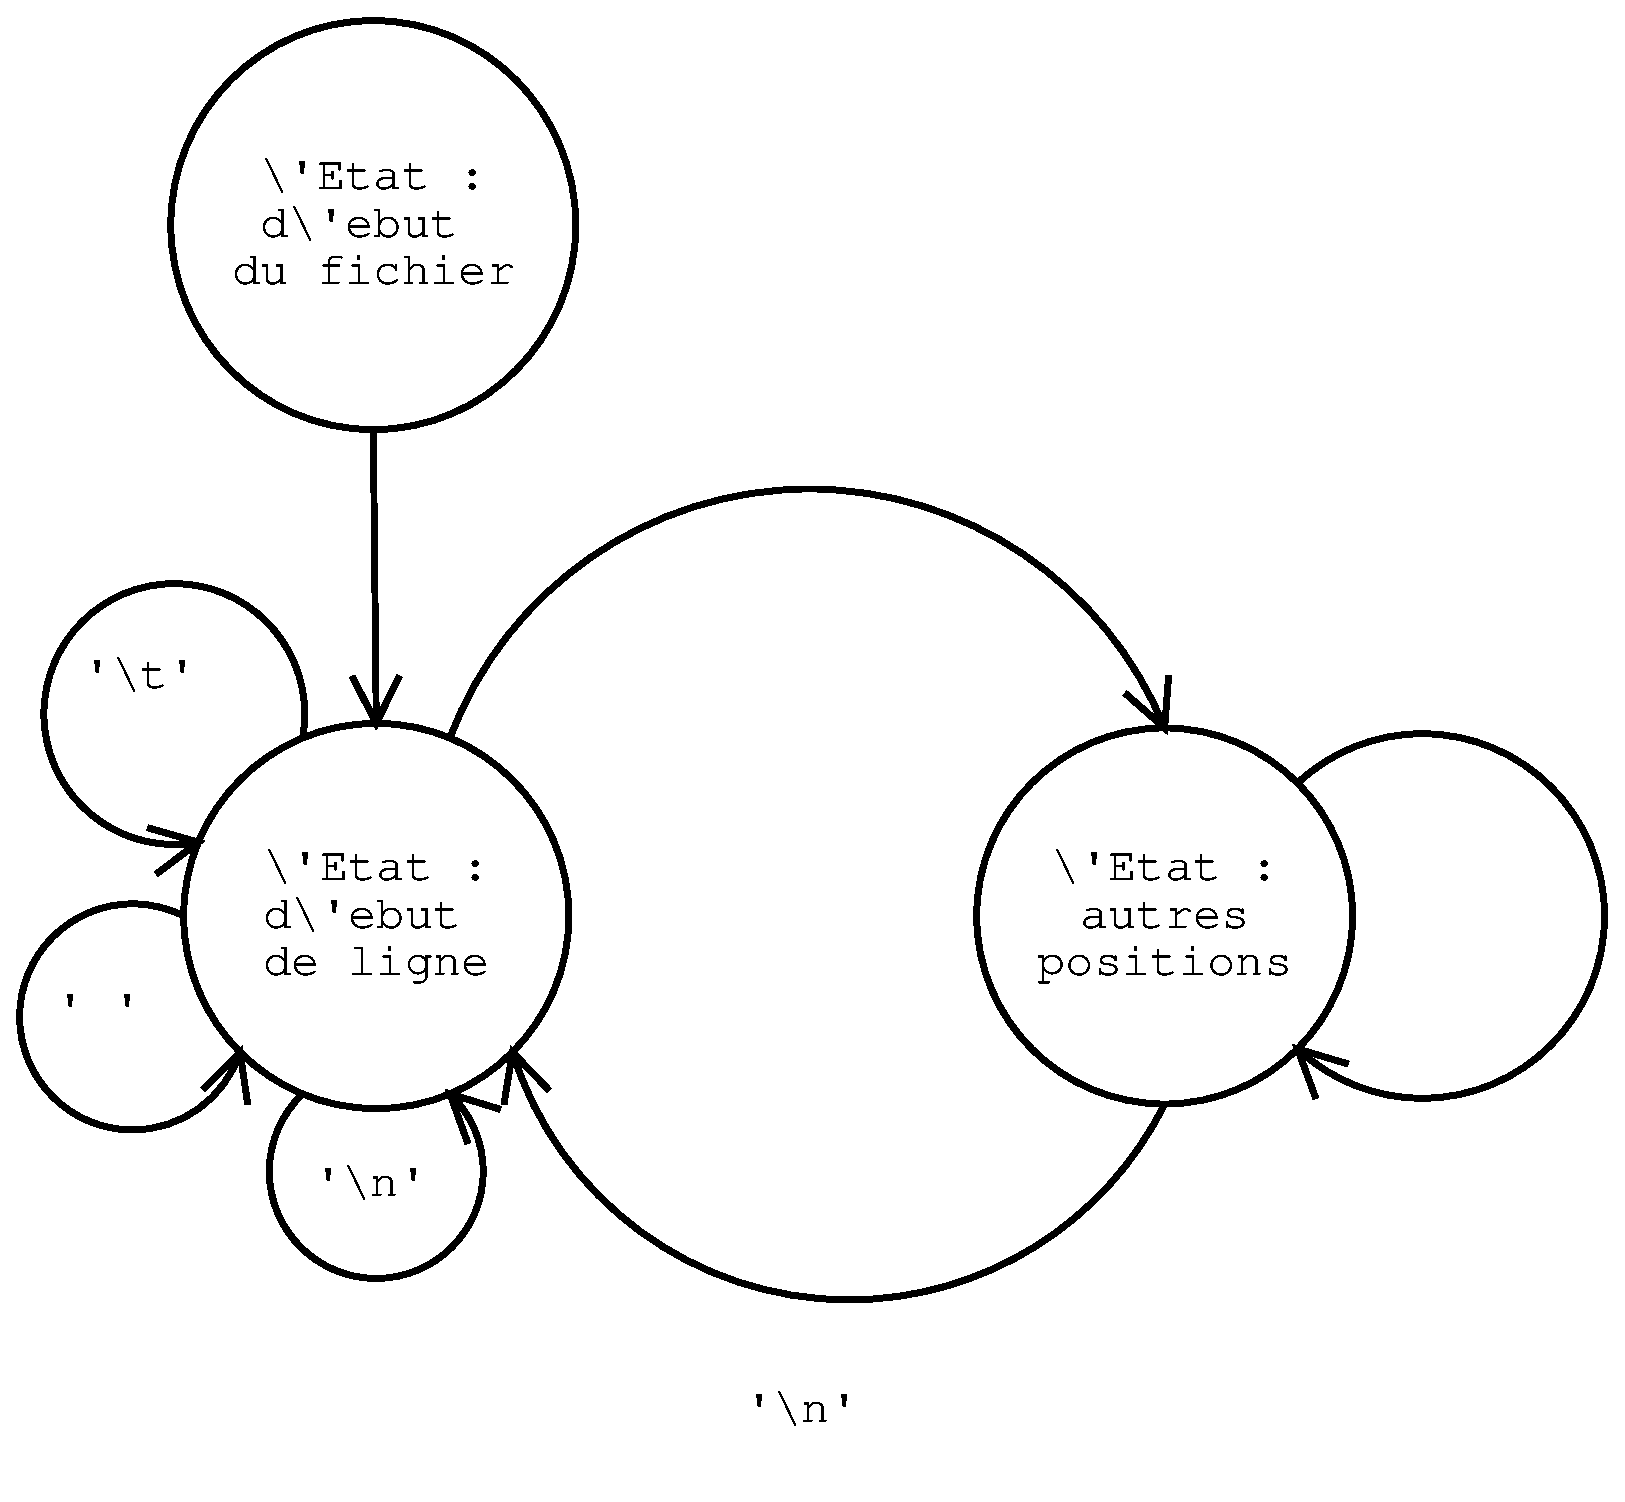
\includegraphics[scale=.3]{../Illustration/automatepp}  
%END LATEX
%HEVEA  \epsfbox{automatepp.ps}  
\end{center}
\begin{exercice}[Construction d'un programme \`a partir d'un automate]
  Inspirez vous de cet automate pour \'ecrire un filtre qui supprime
  les espaces ou les tabulations en d\'ebut de chaque ligne.
   \ifcorrection%
   \begin{correction}
\begin{verbatim}
     #include <stdio.h>
#include <stdlib.h>

int 
main()
{
    int c;
    enum {ETAT_DBT_LIGNE, ETAT_NORMAL } etat = ETAT_DBT_LIGNE;
  
    while ((c=getchar()) != EOF) {
        switch (etat) {
            case ETAT_DBT_LIGNE:
                switch (c) {
                    case ' ':
                    case '\t':
                        break;
                    default:   
                        putchar(c);
                        etat = ETAT_NORMAL;
                        break;
                }
                break;
            case ETAT_NORMAL:
                switch (c) {
                    case '\n': 
                        putchar('\n');
                        etat=ETAT_DBT_LIGNE;
                        break;
                    default :  
                        putchar(c);
                        break;
                }
        }
    }

    exit(EXIT_SUCCESS);
}
\end{verbatim}
   \end{correction}
   \fi%
\end{exercice}

\subsection{Le travail restant \`a faire}
Construisez l'automate codant nos r\`egles de styles et implantez le.


%------------------------------------------------------------------------------
\chapter{Fonctions et r\'ecursivit\'e}
\label{cha:Recursivite}
\section{Introduction aux fonctions}
\label{sec:Fonction}
\begin{exercice}[Fonctions de saisie et d'affichage]
  Reprenez les deux exercices du d\'ebut de la
  section~\ref{sec:getchar} afin de construire les~$2$ fonctions de
  prototypes~:
\begin{verbatim}
int intscan(void);
void intprint(int);
\end{verbatim}
  que vous utiliserez syst\'ematiquement par la suite en lieu et place
  de printf et scanf. Pensez \`a faire un fichier d'ent\^ete contenant
  leurs prototypes et un objet avec lequel vous lierez vos codes
  ult\'erieurs.
\end{exercice}
\begin{exercice}[Suite de Param\`etres et suite d'expressions]
  Nous avons vu dans l'exercice~\ref{sec:SuiteExpression} la notion de
  suite d'expression.  Lors de l'appel d'une fonction, la suite de
  param\`etres fournis \`a la fonction peut \^etre compos\'ees
  d'expressions~: l'\'evaluation de cette suite de param\`etres se
  fait de droite \`a gauche.
  \par
  Pour illustrer ce point, d\'eterminez ce que retourne le code suivant~:
  \input{Verbatim/fctsuiteexpressions.c.verb}
  Testez votre r\'eponse.
\end{exercice}
%------------------------------------------------------------------------------
\section{R\'ecursivit\'e~: exemples classiques}
\label{sec:Recursivite}
\begin{exercice}[Calcul r\'ecursif de la factorielle]
  Implanter le calcul r\'ecursif de la factorielle.
  \ifcorrection
  \begin{correction}
    \input{Verbatim/factoriellerecur.c.verb}
  \end{correction}
  \fi
\end{exercice}
\begin{exercice}[Suite de Fibonacci]
  La suite de Fibonacci est d\'efinie de  mani\`ere r\'ecursive par la
  relation~:
  $$
  u_{n} = u_{n-1} + u_{n-2}.
  $$
  Cette d\'efinition doit \^etre compl\'et\'ee par une condition d'arr\^et.
  Dans notre cas, si~$n$ est \'egal \`a~$0$ ou~$1$ alors~:
  $$
  u_{0}=u_{1}=1.
  $$
  \par
  Par curiosit\'e, on   peut tracer les  calculs.   Ainsi, si on  veut
  calculer~$u_{4}$  et que  l'on suppose que   le premier terme  de la
  somme est calcul\'e en premier,  on est confront\'e  \`a la suite de
  calculs~:
  \par
  \begin{tabular}{c c c c c c c c ccc}
    Fib(4) &=& &&&Fib(3)& &+& &Fib(2) \\
    &=& &Fib(2)&&+&Fib(1) &+& &Fib(2) \\
    &=& Fib(1)&+&Fib(1)&+&Fib(1) &+& &Fib(2) \\
    &=& 1&+&Fib(1)&+&Fib(1) &+& &Fib(2) \\
    &=& 1&+&1&+&Fib(1) &+& &Fib(2) \\
    &=& &2&&+&Fib(1) &+& &Fib(2) \\
    &=& &2&&+&1 &+& &Fib(2) \\
    &=& &&&3& &+& &Fib(2) \\
    &=& &&&3&  &+& Fib(1)&+&Fib(1) \\
    &=& &&&3&  &+& 1&+&Fib(1) \\    
    &=& &&&3&  &+& 1&+&1 \\   
    &=& &&&3&  &+& &2\\
    &=& &&&5 
  \end{tabular}
  \par
  Construire un   programme qui  calcul  r\'ecursivement  le~$n$i\`eme
  terme de la suite de Fibonacci.
  \ifcorrection
\begin{correction}
  \input{Verbatim/fibonaccirecur.c.verb}
\end{correction}
\fi
\paragraph{Remarque.}
Pour m\'emoire,  comptons  le nombre d'appel  r\'ecursifs~$a_{n}$ pour
cette fonction.  Par d\'efinition, on a~:
$$
{a_{0}=a_{1}=1}\qquad   \mathrm{et}\qquad {a_{n}=1+a_{n-1}+a_{n-2}}
\qquad  \mathrm{pour}\qquad {n>1}.
$$
Par changement de variable~${b_{n}=a_{n}+1}$, on en d\'eduit que~:
$$
{b_{0}=b_{1}=2}\qquad   \mathrm{et}\qquad {b_{n}=b_{n-1}+b_{n-2}}
\qquad  \mathrm{pour}\qquad {n>1}.
$$
On  a  donc~$b_{n}=2Fib_{n}$  et  ainsi,~$a_{n}=2Fib_{n}-1$.   Or
si~$\phi$  d\'esigne   le nombre  d'or~${(\sqrt{5}+1)/2}$,          le
terme~$Fib_{n}$ de  la suite de Fibonacci  est l'entier le plus proche
de~${\phi^{n}/\sqrt{5}}$.   Le  nombre  d'appels r\'ecursifs est  donc
exponentiel en~$n$.  Comparez ce  nombre avec le nombre d'it\'erations
n\'ecessaires pour calculer la suite de Fibonacci.
\par
Ce comportement n'est pas la r\`egle  en mati\`ere de r\'ecursivit\'e. 
L'\'ecriture   r\'ecursive  tout  en  \'etant  synth\'etique   peut se
r\'ev\'eler efficace.
\end{exercice}
%------------------------------------------------------------------------------
\begin{exercice}[La fonction~$91$ de MacCarthy]
  Pour    tout  entier~$n$,     MacCarthy  a  d\'efini  la    fonction
  r\'ecursive~$f$ suivante~:
  $$
  f(n) = 
  \begin{array}{l}
    n - 10\ \mathrm{si}\ n> 100 \\
    f(f(n+11))\ \mathrm{sinon}.
  \end{array}
  $$
  Pour  tout~$n$,     cette fonction   vaut~${n-10}$  si~$n$   est
  strictement sup\'erieur  \`a~$100$.  Quelle  est sa valeur  pour~$n$
  inf\'erieur  ou   \'egal \`a~$100$~?  Pour   le  savoir, vous pouvez
  implanter cette fonction.%
  \ifcorrection
  \begin{correction}
    \input{Verbatim/MacCarthy.c.verb}
  \end{correction}
  \fi
\paragraph{Attention.}
Il     n'est pas   \'evident  en~C  qu'une    fonction d\'efinie   par
r\'ecursivit\'e imbriqu\'ee soit  correcte. Prenons  comme exemple, la
fonction de Morris~:
\begin{verbatim}
int Morris(int a, int b){
  if (a == 0)
    return 1 ;
  else 
    return Morris(a-1,Morris(a,b)) ;
}
\end{verbatim}
Que   vaut    \texttt{Morris(1,0)}~?     Par    construction,  on    a
\texttt{Morris(1,0)=Morris(0,Morris(1,0))}.  Puisqu'en~C  le  passage
  d'argument se fait  par  valeur, cette d\'efinition  r\'ecursive  ne
  termine pas.
\end{exercice}
%------------------------------------------------------------------------------
\begin{exercice}[Implantation r\'ecursive de l'algorithme d'Euclide]
  \index{pgcd!Implantation r\'ecursive}
  Implanter une proc\'edure  r\'ecursive permettant le  calcul du plus
  grand commun d\'enominateur (cf.~\ref{ex:AlgorithmeEuclideIteratif}).
  \ifcorrection
  \begin{correction}
    \input{Verbatim/algoEuclideRec.c.verb}
  \end{correction}
  \fi
  D\'eterminer le  nombre d'appels r\'ecursifs n\'ecessaire  au calcul
  du pgcd de~$a$ et~$b$ en fonction de~$a$.
\end{exercice}
\begin{exercice}[le jeu des Tours de Hano\"\i{}]
\label{sec:TourDeHanoi}
En~$1883$, \'Edouard Lucas (1842--91) publie sous le nom de Claus de
Siam  professeur au coll\`ege de Li-Sou-Tsian  ---  anagramme de Lucas
d'Amiens    professeur  \`a Saint-Louis  ---    le   jeu des Tours  de
Hano\"\i{}.    Le  jeu est  constitu\'e   de  trois  piquets verticaux
---~$1$,~$2$ et~$3$ ---     et  de disques superpos\'es   de   tailles
strictement   d\'ecroissantes  enfil\'es autour  du  piquet~$3$~;  ces
disques forment les fameuses tours.
\begin{figure}[htbp]      % Les tours de Hanoi
  \begin{center}
    %BEGIN IMAGE
    \count0=100                 % \count0 la hauteur de la fen\^etre
    \count2=4                  % \count2 le nombre de disques dans la tour

    \count3=\count2            % \count3 le nombre d'\'equivalent disques 
    \advance\count3 by 4       % tenant dans la fen\^etre

    \count4=\count0
    \divide\count4 by \count3  % la largeur d'un disque 

    \count1=\count2            % \count1 la largeur de la fen{\^e}tre 
    \multiply\count1 by 6     
    \advance\count1 by 4    
    \multiply\count1 by \count4 % 

    \count5=\count2
    \advance\count5 by 1 
    \count6=\count4
    \multiply\count6 by \count5  % la position du premier piquet

    \count7=\count4 
    \multiply\count7 by \count5        
    \multiply\count7 by 3        % la position du second piquet 

    \count8=\count4 
    \multiply\count8 by \count5        
    \multiply\count8 by 5        % la position du troisi\`eme piquet 

    \count9=\count4 
    \multiply\count9 by \count2
    \advance\count9 by \count4
    \advance\count9 by \count4   % la hauteur des piquets
    \begin{picture}(\count1,\count0)
      % Premier disque sur le premier piquet
      \count13=\count9                    % la hauteur libre du piquet
      \count10=\count4                    % l'abscisse du coin gauche bas 
      \count11=\count4                    % l'ordonn\'ee du coin gauche bas 
      \count12=\count4                    
      \multiply\count12 by 4              % le num\'ero du disque 
      \multiply\count12 by 2              % le diam\`etre du disque
      \put(\count10,\count11){\framebox(\count12,\count4)}
      \advance\count13 by -\count4
      % Second disque sur le premier piquet
      \advance\count10 by \count4         % l'abscisse du coin gauche bas 
      \advance\count11 by \count4         % l'ordonn\'ee du coin gauche bas 
      \count12=\count4                    
      \multiply\count12 by 3              % le num\'ero du disque 
      \multiply\count12 by 2              % le diam\`etre du disque
      \put(\count10,\count11){\framebox(\count12,\count4)}
      \advance\count13 by -\count4
      % Troisi\`eme disque sur le premier piquet
      \advance\count10 by \count4         % l'abscisse du coin gauche bas 
      \advance\count11 by \count4         % l'ordonn\'ee du coin gauche bas 
      \count12=\count4                    
      \multiply\count12 by 2              % le num\'ero du disque 
      \multiply\count12 by 2              % le diam\`etre du disque
      \put(\count10,\count11){\framebox(\count12,\count4)}
      \advance\count13 by -\count4
      % Quatri\`eme disque sur le premier piquet
      \advance\count10 by \count4         % l'abscisse du coin gauche bas 
      \advance\count11 by \count4         % l'ordonn\'ee du coin gauche bas 
      \count12=\count4                    
      \multiply\count12 by 1              % le num\'ero du disque 
      \multiply\count12 by 2              % le diam\`etre du disque
      \put(\count10,\count11){\framebox(\count12,\count4)}
      \advance\count13 by -\count4
      % dessin du premier piquet
      \advance\count11 by \count4
      \put(\count6,\count11){\vector(0,1){\count13}}
      \put(\count6,0){\makebox(0,0){1}}

      % dessin du second piquet
      \put(\count7,\count4){\vector(0,1){\count9}}
      \put(\count7,0){\makebox(0,0){2}}
      % dessin du troisi\`eme piquet
      \put(\count8,\count4){\vector(0,1){\count9}}
      \put(\count8,0){\makebox(0,0){3}}
      % les disques sur le second piquet
      % les disques sur le troisi\`eme piquet
    \end{picture}     
    %END IMAGE
    %HEVEA \imageflush
    \caption{L'\'etat initial du jeu des Tours de Hano\"\i{} pour~${n=4}$}
    \label{fig:ToursHanoiEtatInitial}
  \end{center}
\end{figure}
Il  faut  d\'eplacer  l'ensemble  des   disques  pour que  ceux-ci  se
retrouvent enfil\'es autour  du piquet~$3$ en  respectant les r\`egles
suivantes~:
\begin{itemize}
\item les disques sont d\'eplac\'es un par un~;
\item un disque ne  doit pas se retrouver  au-dessus d'un  disque plus
  petit.
\end{itemize}
Lucas  a  montr\'e que le  probl\`eme est  toujours r\'esoluble et que
pour une  tour de~$n$ \'etages, il  faut au  minimum~${2^{n}-1}$ coups
pour d\'eplacer la tour. La l\'egende veut que les bonzes d'Hano\"\i{}
passaient leur vie \`a r\'esoudre ce probl\`eme pour~${n=127}$, ce qui
leur permettait d'attendre l'\'ecroulement du temple de Brahma et donc
la  fin du monde.    Pour  m\'emoire,~${2^{127}-1}$ est un nombre   de
Mersenne dont Lucas a d\'emontr\'e la primalit\'e.
\paragraph{Raisonnement par r\'ecurrence}
L'id\'ee de la  r\'ecursivit\'e telle que nous l'employons aujourd'hui
est attribuable \`a   Stephan~C.\ Kleene (1909--94)  notion  offre une
solution \'el\'egante au probl\`eme des Tours de Hano\"\i{}.
\paragraph{Principe.}
Supposons  notre probl\`eme  r\'esolu  pour~${n-1}$ disques  i.e.\ que
l'on sache  transf\'erer~${n-1}$ disques depuis le piquet~$i$ jusqu'au
piquet~$j$ en  respectant les  r\`egles du  jeu.  Il existe  alors une
solution simple pour  transf\'erer~$n$    disques  dans  les   m\^emes
conditions~:
\begin{enumerate}
\item  on  am\`ene les~${n-1}$ disques   du haut du  piquet~$i$ sur le
  troisi\`eme piquet --- repr\'esent\'e par~${6-(i+j)}$~;
\item on prend  le dernier  disque  du piquet~$i$  et  on le  met seul
  en~$j$~;
\item on ram\`ene les~${n-1}$ disques de~${6-(i+j)}$ en~$j$.
\end{enumerate}
\paragraph{Implantation.}
Construire une  fonction  {\tt  Hanoi.c}   qui permet  d'afficher  les
mouvements  \'el\'ementaires \`a accomplir pour d\'eplacer~$n$ disques
du piquet~$i$ au piquet~$j$  (une proc\'edure principale est fournie). 
Utiliser  cette fonction   dans    un  programme~C qui  demande    \`a
l'utilisateur le nombre de disque \`a placer sur le premier piquet et
qui affiche une solution du jeu.%
\ifcorrection
\begin{correction}
\input{Verbatim/Hanoi.c.verb}
\end{correction}
\fi
\end{exercice}
%------------------------------------------------------------------------------
\begin{exercice}[Le probl\`eme des reines]
  Le probl\`eme  des reines consiste    \`a placer~$n$ reines  sur  un
  \'echiquier de taille~${n\times n}$  de telle sorte  qu'aucune reine
  ne soit en prise~: il ne faut  donc pas plus  d'une reine par ligne,
  par colonne et par diagonale.
  \par
  Voici un exemple de solution pour~${n=8}$~:
  \par
  \begin{tabular}{|c|c|c|c|c|c|c|c|}
    \hline
    &R& & & & & & \\
    \hline
    & & & &R& & & \\
    \hline
    & & & & & &R& \\
    \hline
    & & &R& & & & \\
    \hline
    R& & & & & & & \\
    \hline
    & & & & & & &R\\
    \hline
    & & & & &R& & \\
    \hline
    & &R& & & & & \\
    \hline
  \end{tabular}
  On peut trouver les solutions du probl\`eme  des reines en explorant
  r\'ecursivement  l'espace des  configurations  possibles. Le  but de
  l'exercice sera de compter le  nombre de solutions du probl\`eme des
  reines pour un entier~$n$ donn\'e.
  \par
  Ainsi, pour~${n=1}$, il  y a une seule  configuration, pour~${n=2}$,
  il n'y en a pas, etc.
  \par
  L'algorithme n\'ecessite trois tableaux de bool\'eens repr\'esentant
  les contraintes engendr\'e par le placement des reines. Il y a un tableau qui indique
  \begin{itemize}
  \item pour chaque ligne si elle est d\'ej\`a occup\'ee par une reine~;
  \item pour chaque diagonale ``descendante'' si elle est d\'ej\`a occup\'ee par une reine~;
  \item pour chaque diagonale ``montante'' si elle est d\'ej\`a occup\'ee par une reine.
  \end{itemize}
  Pour la  mise au point  du programme, on  pourra ajouter  un tableau
  pour stocker la solution en cours de construction.
  \par
  L'algorithme consiste  \`a placer une reine  dans  chaque colonne et
  \`a mettre  \`a  jours  les tableaux  ci-dessus.   Il  n'y  a qu'une
  fonction r\'ecursive    \`a \'ecrire.  Elle  prend  en   argument le
  num\'ero~$i$ de la colonne \`a explorer  et les trois tableaux. Elle
  retourne le nombre  de solutions possibles  avec les reines d\`ej\`a
  plac\'ees dans les colonnes~$0$ \`a~${i-1}$.
\end{exercice}

%------------------------------------------------------------------------------
\chapter{Tableaux~: tables, recherches et tris}
\label{cha:Tableaux}
\section{Le type tableau}
\label{sec:TypeTableau}
Dans les sections pr\'ec\'edentes, nous avons utilis\'e des variables de type
\textbf{int} et   \textbf{float}.  Ces types   sont qualifi\'es de
\textit{scalaire} car \`a chaque variable est associ\'ee une seule une
information   simple.  Ainsi,  si  on la   d\'eclaration~:~\texttt{int
  A=0;}, la variable \texttt{A} ne contient qu'une seule valeur \`a un
moment donn\'e.      Par    opposition,  une   variable     d'un  type
\texttt{compos\'e} est associ\'ee \`a plusieurs informations.
\subsection{Tableaux monodimensionnel}
\label{sec:Tableaumonodimensionel}
Si on veut stocker un tableau contenant~$n$ entiers dans une variable,
il  nous  faut  tout  d'abord   d\'efinir la   structure  de donn\'ees
correspondante.  Ainsi, on va d\'efinir un tableau \texttt{nom}
\`a~$10$ entr\'ees enti\`eres par la commande~:%
\par
\centerline{\textbf{type}   \texttt{nom}\textbf{[}\texttt{n}\textbf{]}
  \textbf{;}}
\par
On   peut affecter~$7$   \`a la   troisi\`eme  composante du   tableau
associ\'e \`a cette variable par l'instruction~\texttt{var[3]=7;}.  On
peut  affecter  un   tableau  d'entiers  \texttt{var2}   lors  de   sa
d\'eclaration en utilisant l'instruction~:
\begin{verbatim}
int var2[10] = {1,2,3,4,5,6,7,8,9,10} ;
\end{verbatim}
\begin{exercice}[Crible d'\'Eratosth\`ene]
  Construire un programme qui affiche tous les nombres premiers de~$2$
  \`a~$1000$.      Pour  ce  faire,   on   va    utiliser   le  crible
  d'\'Eratosth\`ene~: on construit   un  tableau contenant  tous   les
  entiers de~$2$ \`a~$1000$,  puis on supprime  (par exemple remplacer
  par~$0$) les multiples de~$2$, puis ceux de~$3$, etc.
  \ifcorrection
  \begin{correction}
    \input{Verbatim/crible_Eratosthene.c.verb}
  \end{correction}
  \fi
\end{exercice}
\begin{exercice}[Fr\'equence d'incidence dans un tableau]
  Lors d'une  enqu\^ete de satisfaction pour  un produit,  des clients
  \'etaient invit\'es \`a donner une note enti\`ere entre~$0$ et~$20$.
  Les~$500$    r\'eponses ont  \'et\'e    collect\'ees dans un tableau
  d'entiers.
\begin{verbatim}
#define NbNote 500

int resultat[NbNote]={3, 7, 9,  0, 18, 5, 4, 19,  8, 3, 10, 7, 14, 13,
0, 18, 17, 5, 16, 4, 5, 1, 20, 6, 16, 10, 13, 12,  6, 5, 20, 8, 9, 15,
3, 17, 12, 10, 19, 3, 13, 4, 13, 14 , 17, 17, 15, 14, 18, 6, 17, 9, 9,
6, 15, 17, 11, 8, 8, 0, 19,  19, 13, 18, 11, 1,  16, 5, 16, 7, 18, 20,
3, 16, 3, 9, 1, 3, 20, 11, 6, 19, 0, 13, 10, 14, 13,  5, 1, 16, 2, 19,
10, 2, 14, 6, 8, 15, 4, 6, 8, 20, 4, 2, 0, 18,  19, 20, 13, 1, 13, 16,
12, 12, 7, 19, 13, 11, 3, 18, 10, 7, 20, 0, 4, 4, 16, 14, 19, 0, 0, 16,
  4, 0, 7, 18, 15, 8, 8, 6, 1, 12, 17,  9, 1, 4, 13,  0, 8, 15, 19, 4,
3, 1, 3, 1, 1, 1, 6, 10, 15, 8, 14, 17, 14, 3, 5, 0, 19, 6, 8, 13, 14,
2, 1, 12, 4, 1, 10, 17, 11, 7,  11, 12, 6, 10,  8, 18, 13, 15, 12, 14,
8, 2, 2, 3, 17, 6,  9, 17, 9, 19,  16, 8, 18, 0, 10,  15, 2, 17, 2, 3,
13, 19, 13, 12, 12, 2, 2, 4, 17, 17, 17, 2, 11, 19, 13, 8, 0, 9, 8, 5,
4, 13, 9, 9, 19, 15, 19, 1, 19, 10, 20, 1, 11, 8,  13, 0, 10, 6, 5, 1,
11, 0, 8, 13, 5, 0, 15, 9, 7, 0, 10, 0, 1,  12, 12, 10,  19, 17, 0, 6,
16, 12, 8, 12, 14, 13, 15, 20, 7, 17, 1, 18, 15, 13, 6, 14, 18, 8, 13,
14, 8, 14, 7, 16, 2, 19, 14, 6, 17, 8, 11, 14, 16, 11,  19, 2, 20, 16,
2, 13, 14, 20, 6, 13, 20, 9, 3, 19, 3, 0, 7, 0, 16,  7, 4, 15, 16, 17,
2, 14, 3, 15, 12, 16, 18, 1, 5,  9, 2, 1, 5, 9,  5, 13, 10, 11, 16, 6,
16, 8, 13, 11, 6, 8, 2, 5, 2, 5, 9, 1,  7, 20, 19, 4, 14,  2, 8, 9, 5,
9, 9, 5, 15, 12, 3, 7, 15, 17, 6, 0, 7, 2, 17, 19,  20, 15, 1, 11, 11,
18, 9, 7, 1, 1, 17, 1, 17, 10, 2, 5, 1,  14, 7, 2, 3, 0,  4, 2, 9, 17,
3, 6, 7, 18, 14, 14,  4, 10, 3, 15,  16, 17, 6, 15, 12,  17, 9, 5, 14,
14, 6, 4, 4, 4, 17, 10, 10, 11, 13, 16, 3, 0, 2, 18, 3,  20, 5, 16, 6,
0, 8, 3, 3, 10, 2, 0, 6, 11, 12, 9, 18, 8, 6, 2, 0, 0,  19, 12, 17, 5,
19, 12, 17, 4, 0, 20, 8, 3, 7,  6, 10, 0,  3, 4, 4,  6, 11, 0, 13, 14,
17, 20, 12, 3, 18, 3, 13, 14 };
\end{verbatim}
  Construisez une proc\'edure qui  permet d'afficher les notes qui  ont
  \'et\'e donn\'ees  le  plus et   le   moins souvent ainsi  que   les
  fr\'equences  correspondantes.    De plus, affichez   un histogramme
  horizontal des fr\'equences des notes donn\'ees en entr\'ees.
  \par
  \textbf{Indications.} Pour ce   faire,   on va cr\'eer    un tableau
  de~$21$  \'el\'ements  indic\'e  de~$0$   \`a~$20$ dont la~$n$i\`eme
  composante contiendra  le nombre de fois  o\`u la note~$i$ a \'et\'e
  donn\'ee.  Ensuite,  il  nous faudra d\'eterminer  le  maximum et le
  minimum de ce tableau  et en d\'eduire les notes  les plus et  moins
  fr\'equentes.
  \par
  L'exemple  a \'et\'e choisi  afin que le  maximum  et le minimum des
  fr\'equences soient uniques.
  \ifcorrection
  \begin{correction}
    \input{Verbatim/frequencenote.c.verb}
  \end{correction}
  \fi
\end{exercice}
\subsection{Tableaux bidimensionnel}
\label{sec:TableauMultidimensionel}
Un tableau peut  \^etre multidimensionnel et coder une matrice~$6$x$6$
\`a coefficients flottant.
\par
On  peut d\'efinir  le tableau  \`a  deux dimensions correspondant par
l'instruction~:
\begin{verbatim}
float matrice[6][6];
\end{verbatim}
et   affecter   \`a~$1$   le  coefficient~${(i,j)}$  de   la  variable
\texttt{matrice}   par     l'instruction~\texttt{matrice[i][j]=1;}.    
Remarquons  que  l'on peut d\'eclarer  et  affecter la matrice~$2$x$2$
identit\'e              par            l'instruction~:
\begin{verbatim}
int id[2][2]={{1,0},{0,1}};
\end{verbatim}
\begin{exercice}[Matrice~: saisie, produit et affichage]
  \'Ecrivez    une proc\'edure      qui   permet    de  saisir    deux
  matrices~$3$x$3$, de faire leurs produit et de l'afficher.
  \ifcorrection
  \begin{correction}
    \input{Verbatim/matrice.c.verb}
  \end{correction}
  \fi
\end{exercice}
\begin{exercice}[Jeu de la vie]
  Le  jeu  de la vie  a  \'et\'e \'elabor\'e par  John~H.\  Conway. On
  consid\`ere un tableau bidimensionnel    dont chaque  cellule   peut
  \^etre dans l'un des deux \'etats suivants~:
  \begin{itemize}
  \item occup\'ee (par une cellule vivante)~;
  \item vide (cellule morte).
  \end{itemize}
  Chacune des huits cases  qui  entourent une  case donn\'ee  est dite
  \textit{adjacente} ou \textit{voisine}.
  Les r\`egles du jeu sont les suivantes~:
  \begin{enumerate}
  \item \textbf{R\`egle de  la survie~:} chaque cellule vivante ayant,
    \`a l'\'etape~$n$, deux  ou  trois  cellules  vivantes  adjacentes
    survit \`a l'\'etape~${n+1}$~;
  \item \textbf{R\`egles  de  la mort~:} chaque  cellule vivante ayant
    pour voisines,   \`a   l'\'etape~$n$,  quatre  cellules   vivantes
    adjacentes ou plus, dispara\^\i{}t \`a l'\'etape~${n+1}$ (mort par
    surpopulation).   Une  cellule vivante   n'ayant qu'une  ou aucune
    cellule vivante adjacente meurt  \`a l'\'etape suivante  (mort par
    isolement)~;
  \item \textbf{R\`egle  de naissances~:}  chaque cellule  morte ayant
    exactement trois  cellules   vivantes   adjacentes, engendre   \`a
    l'\'etape suivante une cellule vivante.
  \end{enumerate}
  Le jeu de la vie est un  exemple d'automate cellulaire.  Nous allons
  construire un programme  permettant  d'initialiser, de repr\'esenter
  les \'etats, de g\'erer et d'afficher cet automate.
  Pour ce faire, il nous faut~:
  \begin{itemize}
  \item repr\'esenter les  cellules par un tableau bidimensionnel  (le
    plan de jeu). Le  plan du jeu  est suppos\'e infini.  Il nous faut
    donc le repr\'esenter par  un tore de taille~${20\times 20}$ (pour
    fixer  les id\'ees).  Pour  travailler dans  ce tore, vous  pouvez
    supposer que les coordonn\'ees sont dans un corps fini et utiliser
    le reste de la division euclidienne \texttt{\%}~;
  \item initialiser ce tableau~;
  \item construire  un code qui  permet  la transition d'un \'etat  au
    suivant (n'oubliez pas  que cette transition n\'ecessite une copie
    du plan de jeu~;
  \item construire du code qui permettent l'affichage.
  \end{itemize}
  Pour tester votre programme voici quelques configurations classiques~:
  \begin{itemize}
  \item le clignotant
\begin{verbatim}
     
 XXX 
     
\end{verbatim}
  \item le glisseur
\begin{verbatim}
     
  X  
   X 
 XXX 
     
\end{verbatim}
  \item le t\'etramino
\begin{verbatim}
     
 XXX 
  X  
     
\end{verbatim}
  \item le goinfre
\begin{verbatim}
      
   XX 
    X 
 XXX  
 X    
      
\end{verbatim}
  \end{itemize}
  Enfin, vous pouvez choisir des  conditions initiales al\'eatoires en
  utilisant la fonction \texttt{random()} (cf.\ \texttt{man random}).
  \Ifcorrection
  \begin{correction}
    \input{Verbatim/JeuDeLaVie.c.verb}
  \end{correction}
  \fi
\end{exercice}
%------------------------------------------------------------------------------
\section{Recherche en table}
\label{sec:RechercheEntable}
Une table  contient   des informations  sur   certaines  clefs.   Dans
l'exemple suivant, les clefs  sont des abr\'eviations et l'information
est  constitu\'ee par le sens   des ces abr\'eviations.  L'instruction
\texttt{char bar[32]="foo"} d\'efinit une  variable \texttt{bar} et on
lui affecte la cha\^\i{}ne de  caract\`eres \texttt{``foo''}. On  peut
donc d\'efinir deux tableaux~:
\begin{verbatim}
#define N 100

char *ABR[N] ;
char *EXP[N] ;

int NbTotal = 13 ;

ABR[1]="ANSI";
EXP[1]="American National Standards Institute";
ABR[2]="ASCII";
EXP[2]="American Standard Code for Information Interchange";
ABR[3]="BIOS";
EXP[3]="Basic Input/Output System";
ABR[4]="GRUB";
EXP[4]="Grand Unified Bootloader";
ABR[5]="IDE";
EXP[5]="Integrated Drive Electronics";
ABR[6]="ISA";
EXP[6]="Instruction Set Architecture";
ABR[7]="ISO";
EXP[7]="International Standards Organization";
ABR[8]="OS";
EXP[8]="Operating System";
ABR[9]="PCI";
EXP[9]="Peripheral Component Interconnect";
ABR[10]="ROM";
EXP[10]="Read Only Memory";
ABR[11]="RTFM";
EXP[11]="Read The F... Manuel";
ABR[12]="SCSI";
EXP[12]="Small Computer System Interface";
ABR[13]="VLSI";
EXP[13]="Very Large Scale Integration";
\end{verbatim}
Une table peut \^etre construite \`a partir d'une liste ou d'un arbre.
Pour l'instant, nous allons utiliser deux tableaux --- \texttt{ABR} et
\texttt{EXP}  --- indic\'es en   parall\`ele pour coder  notre table~:
l'abr\'eviation de \texttt{EXP[i]} \'etant \texttt{ABR[i]}.
\par
La table ci-dessus  peut contenir~$100$ \'el\'ements au maximum  mais,
on n'utilise que~$nbtotal$  cellules.  On ne  g\`ere pas ici la taille
courante de  la table dans notre  exemple par une  variable car  on se
propose    d'utiliser une \textit{sentinelle}   en  bout  de table qui
indique qu'apr\`es elle, il n'y a plus de cellule affect\'ee.
\subsection{Recherche s\'equentielle}
\label{sec:RechercheSequentielle}
La premi\`ere  m\'ethode  pour rechercher le sens  d'une abr\'eviation
est  d'examiner successivement tous les  \'el\'ements de  la table. Il
s'agit  d'une  recherche s\'equentielle~; cette  recherche  est  aussi
qualifi\'ee de   lin\'eaire    parce que le   nombre    d'op\'erations
n\'ecessaires est lin\'eaire dans la taille de la table.
\begin{exercice}[Recherche s\'equentielle]
  \'Ecrivez une  proc\'edure  bas\'ee sur  la recherche s\'equentielle
  qui  affiche le sens d'une abr\'eviation  saisie au clavier tant que
  l'utilisateur le demande.
  \par
  Il faut  noter que  
  \begin{itemize}
  \item si la variable \texttt{chaine} est d\'efinit par l'instruction
    \texttt{char  *chaine}, la  fonction \texttt{scanf}  s'utilise par
    l'appel   \texttt{scanf("\%s",chaine)} (ce  point sera  \'eclairci
    dans la section~\ref{cha:Pointeurs})~;
  \item  l'\'egalit\'e de deux  cha\^\i{}nes  de caract\`eres se teste
    \`a l'aide de  la  fonction \texttt{strcmp}.  Cette  fonction  est
    d\'efinie  dans la  librairie  \texttt{string.h}~; elle   prend en
    argument   deux  cha\^\i{}nes de   caract\`eres et retourne~$0$ si
    elles sont identiques, une valeur positive  si le premier argument
    est plus grand que le second et une valeur  n\'egative dans le cas
    contraire.  N'h\'esitez     pas  \`a utiliser  le   manuel  d'unix
    \texttt{man strcmp} \`a partir de votre shell.
  \item la conditionnel  \texttt{if} consid\`ere qu'une expression est
    fausse     si elle  retourne~$0$.   La   boucle  for  ex\'ecute  les
    instructions  sp\'ecifi\'ees tant  que  la seconde expression  est
    fausse~;
  \end{itemize}
  \ifcorrection
  \begin{correction}
    \input{Verbatim/rechercheSequentielle.c.verb}
  \end{correction}
  \fi
\end{exercice}
\par
\paragraph{Insertion d'\'el\'ements}
Si on  utilise  une recherche s\'equentielle dans  une  table, on peut
rajouter  des  \'el\'ements nouveaux en  bout  de  table et produire une
erreur s'il n'y  a plus de place.   Afin que cette op\'eration  puisse
\^etre  r\'ealis\'ee  en   temps constant  (ne  pas  n\'ecessiter  de
parcours dans  la table),  on  se  doit  d'utiliser  une variable  qui
indique la derni\`ere cellule affect\'ee. 
\begin{exercice}[Recherche s\'equentielle avec insertion d'\'el\'ements]
  Modifiez votre programme afin  que l'utilisateur puisse ins\'erer  ses
  propres donn\'ees dans la table.
\end{exercice}
\subsection{Recherche dichotomique}
\label{sec:RechercheDichotomique}
Supposons  que la table soit  tri\'ee en ordre alphab\'etique. On peut
alors utiliser une   recherche dichotomique pour  explorer notre table
i.e.\ utiliser la m\'ethode suivante~:
\begin{enumerate}
\item on compare  notre cl\'e \`a une abr\'eviation  qui se trouve au
  milieu de la table des abr\'eviations~;
\item si c'est la m\^eme, on retourne son  sens tir\'e de la table des
  expressions~;
\item   sinon, on recommence l'\'etape~$1$  sur  la premi\`ere (resp.\ 
  seconde) moiti\'e  de table  si  le nom  recherch\'e est  plus petit
  (resp.\ plus grand) que le nom rang\'e au milieu de la table.
\end{enumerate}
\begin{exercice}[Recherche dichotomique]
  \'Ecrivez une proc\'edure bas\'ee  sur la recherche dichotomique qui
  affiche le  sens d'une   abr\'eviation  saisie au clavier   tant que
  l'utilisateur le demande.
  \ifcorrection
  \begin{correction}
    \input{Verbatim/rechercheDichotomique.c.verb}
  \end{correction}
  \fi
\end{exercice}
\paragraph{Remarques sur la complexit\'e}
\begin{itemize}
\item Notons~$u_{n}$ le nombre de  comparaisons n\'ecessaires pour une
  table   de taille~$n$.  On  a~${u_{1}=1}$ et~${u_{n}=1+u_{n/2}}$. Le
  nombre~$u_{n}$ est   logarithmique dans la  taille~$n$  de la table. 
  C'est donc   une   am\'elioration  par   rapport \`a    la recherche
  s\'equentielle~;
\item  Si on veut ins\'erer un  nouvel \'el\'ement  dans la table afin
  d'effectuer une   recherche dichotomique,  cette  derni\`ere  devant
  \^etre ordonn\'ee, il  nous faut trouver  sa place dans la table  et
  d\'eplacer tous les  \'el\'ements  plus grand. On retombe  ainsi sur
  une complexit\'e lin\'eaire en la taille de la table.
\end{itemize}
%------------------------------------------------------------------------------
\section{Tris s\'equentiels}
\label{sec:TrisSequentiels}
Dans la suite, on consid\`ere un dictionnaire de mots de quatre lettres.
\input{Verbatim/dico4lettres.h.verb}
Ce dictionnaire  est  stock\'e dans  une  variable  globale  et on  se
propose de le trier.
\par
Pour ce faire,   on  rappelle qu'il est    possible de comparer   deux
cha\^\i{}nes de caract\`eres en  utilisant la fonction \texttt{strcmp}
dont   la  d\'eclaration  est   dans   \texttt{string.h} (pour plus   de
d\'etails, \texttt{man strcmp}).
\subsection{Tri par s\'election}
\label{sec:TriSelection}
L'algorithme de tri le  plus simple consiste \`a trouver l'emplacement
du plus petit \'el\'ements dans  la table consid\'er\'ee. Une fois cet
emplacement trouv\'e, on \'echange le  premier \'el\'ement de la table
avec le plus petit. Pour continuer, on recommence ces op\'erations sur
la table compos\'ee des \'el\'ements restant.
\begin{exercice}[Tri par s\'election]
  Implantez le tri par s\'election de la  table \texttt{dico}. Pour ce
  faire,  construisez une    fonction principale   et deux   fonctions
  auxiliaires (recherche du plus petit \'el\'ement et tri).%
  \ifcorrection
  \begin{correction}
    \input{Verbatim/TriSelection.c.verb}
  \end{correction}
  \fi
\paragraph{\'Etude de la complexit\'e.}
\`A  chaque it\'eration~$i$,     on compare  l'\'el\'ement~$i$     \`a
l'\'el\'ement class\'e apr\`es lui.  Si~$t$  repr\'esente la taille de
la  table, on fait     donc~${t-i}$ comparaisons.  Comme  il  y  a~$t$
it\'erations, on a~${t(t-1)/2}$ comparaisons et~${n-1}$ \'echanges. La
complexit\'e est donc de l'ordre de~$t^{2}$.
\end{exercice}
\subsection{Tri bulle}
\label{sec:TriBulle}
\begin{exercice}[Tri bulle]
  Le  tri  bulle  consiste \`a     parcourir  la table  \`a trier   en
  intervertissant   toute   paire  d'\'el\'ements   cons\'ecutifs  non
  ordonn\'es afin qu'apr\`es un parcours, le plus grand \'el\'ement se
  retrouve \`a la  fin de la   table. On recommence cette  op\'eration
  avec la table consid\'er\'ee sans le dernier \'el\'ements.
  \par
  Implantez un tri bulle.%
  \ifcorrection
  \begin{correction}
    \input{Verbatim/TriBulle.c.verb}
  \end{correction}
  \fi
\end{exercice}
\subsection{Tri par insertion}
\label{sec:TriParInsertion}
\begin{exercice}[Tri par insertion]
  Dans la m\'ethode du tri par insertion, on ordonne les deux premiers
  \'el\'ements de la table. Puis, on  consid\`ere le troisi\`eme et on
  le met \`a sa  place parmi les  deux premiers. Ainsi, on consid\`ere
  les~${j-1}$ premiers  \'el\'ements de  la  table comme tri\'es.   On
  prend la~$j$i\`eme et on le met \`a sa place dans la partie d\'ej\`a
  tri\'ee.
  \ifcorrection
  \begin{correction}
    \input{Verbatim/TriInsertion.c.verb}n
  \end{correction}
  \fi
\end{exercice}
\subsection{Tri Shell}
\label{sec:TriShell}
\begin{exercice}[Tri Shell]
  Une variante du  tri par insertion  a \'et\'e introduite par D.~L.\ 
  Shell en~$1959$. Le principe est de supposer  que la table \`a trier
  est \textit{presque} en ordre. Au lieu  de comparer les \'el\'ements
  adjacents  pour   l'insertion, on  les   compares  tous  les~$u_{n}$
  \'el\'ements avec~${u_{n+1}=3u_{n}+1}$.
  \par
  Implantez un tri shell.%
  \ifcorrection
  \begin{correction}
    \input{Verbatim/TriShell.c.verb}
  \end{correction}
  \fi
\end{exercice}
\section{Tris r\'ecursifs}
\label{sec:TrisRecursifs}
\subsection{Quicksort}
\label{sec:Quicksort}
\begin{exercice}[Quicksort]
  Le tri Quicksort a \'et\'e introduit par C.A.R.~Hoare en~$1960$. Il
  consiste \`a prendre un \'el\'ement au hasard dans le table \`a
  trier.  Soit~$v$ cet \'el\'ement.  On partitionne le reste du
  tableau en deux zones~:
  \begin{enumerate}
  \item les \'el\'ements plus petit ou \'egaux \`a~$v$~;
  \item les \'el\'ements plus grand \`a~$v$.
  \end{enumerate}
  Il  faut maintenant mettre les  \'el\'ements plus  petits ou \'egaux
  \`a~$v$ en  t\^ete de la table, les  \'el\'ements plus grands en fin
  de  table  et mettre~$v$ \`a  sa  place  d\'efinitive entre les deux
  zones.
  \par
  On peut recommencer r\'ecursivement cette  manipulation sur les deux
  partitions ainsi cr\'e\'es tant  qu'elles ne sont pas r\'eduites \`a
  un \'el\'ements.
  \par
  Implanter un tri Quicksort.
  \ifcorrection
  \begin{correction}
    \input{Verbatim/qsort.c.verb}
  \end{correction}
  \fi
\end{exercice}
\subsection{Tri par fusion}
\label{sec:TriParFusion}
Cette notion ne sera pas abord\'ee dans ce cours.

%------------------------------------------------------------------------------
\chapter{Autres types~: \'enum\'erations, types compos\'es}
\label{cha:TypesComposes}
%------------------------------------------------------------------------------
\section{\'Enum\'erations}
\label{sec:Enumerations}
%------------------------------------------------------------------------------
\section{Structures}
\label{sec:Structures}
Une variable  de type  structure est  un ensemble  fini de variable de
types diff\'erents~; ces \'el\'ements sont les champs de la structure.
\par\index{struct}
La d\'eclaration  d'un \textit{type structure}  dont  l'identificateur
est \texttt{modele} suit la syntaxe suivante~:
\begin{verbatim}
typedef struct modele {
        type1 champs1 ;
             ...
        typeN champsN ;
} modele ;
\end{verbatim}
Pour d\'eclarer une  variable \texttt{var} du type \texttt{modele}, on
utilise la syntaxe~: \texttt{struct modele var;}
\par
Si le type \texttt{modele} n'a pas \'et\'e d\'eclar\'e au pr\'ealable,
on utilise la syntaxe~:
\begin{verbatim}
 struct modele {
        type1 champs1 ;
             ...
        typeN champsN ;
} var ;
\end{verbatim}
On   acc\`ede  aux diff\'erents   champs  d'une structure  gr\^ace \`a
l'op\'erateur  \texttt{.}  appel\'e membre  de structure.  Le~$i$\`eme
\'el\'ements de   la structure   \texttt{var}  est accessible    par
l'instruction~: \texttt{var.champsi}.
\par
Les r\`egles d'initialisation d'une structure lors de sa d\'eclaration
sont les m\^emes que pour les tableaux~:
\begin{verbatim}
struct modele var = { int1, ... , initN } ;
\end{verbatim}
Contrairement  aux  tableaux,   on    peut   appliquer   l'op\'erateur
d'affectation aux structure~:
\begin{verbatim}
struct modele var2 = var ;
\end{verbatim}
\begin{exercice}[Implantation de fractions]
Les rationnels peuvent \^etre consid\'er\'es comme un couple d'entiers~:
la fraction~$3/4$ est repr\'esent\'e par le couple d'entiers~$(3,4)$. 
\par
Nous allons  implanter l'arithm\'etique  des fractions rationnelles et
pour ce faire, il nous faut d\'efinir un type \texttt{Rationnel}. Nous
pourrions  utiliser un  tableau  de  deux   entiers mais  nous  allons
plut\^ot utiliser une structure.
\par
Pour implanter notre arithm\'etique, il nous faut coder~:
\begin{itemize}
\item une fonction d'affichage d'un rationnel~: la fonction
  \texttt{PrintRationnel} prend en argument une variable de type
  \texttt{Rationnel} et affiche un rationnel~;
\item l'addition de deux rationnels~: la fonction \texttt{addRationnel} prend
  en argument deux variables de types \texttt{Rationnel} et retourne
  une variable de type \texttt{Rationnel} codant la somme des deux
  arguments~;
\item le produit de deux rationnels~: la fonction \texttt{mulRationnel} prend
  en argument deux variables de types \texttt{Rationnel} et retourne
  une variable de type \texttt{Rationnel} codant le produit des deux
  arguments~;
\item le quotient de deux rationnels~: la fonction \texttt{quoRationnel} prend
  en argument deux variables de types \texttt{Rationnel} et retourne
  une variable de type \texttt{Rationnel} codant le quotient du
  premier argument par le second~;
\item la r\'eduction sous forme irr\'eductible d'un rationnel~: la
  fonction \texttt{normalRationnel} prend en argument une variable de type
  \texttt{Rationnel} et retourne une variable de type
  \texttt{Rationnel} codant la forme irr\'eductible de l'argument (la
  forme irr\'eductible de la fraction~$2/4$ est~$1/2$).
\end{itemize}
\ifcorrection
\begin{correction}
\input{Verbatim/rationnel.c.verb}
\end{correction}
\fi
\end{exercice}
%------------------------------------------------------------------------------
\begin{exercice}[Implantation des nombres complexes]
  Les nombres complexes peuvent  \^etre consid\'er\'es comme un couple
  de r\'eels~:  le  nombre complexe~$3+4I$  est  repr\'esent\'e par le
  couple~$(3,4)$.
\par
Nous allons implanter l'arithm\'etique des complexes et pour ce faire,
il nous faut   d\'efinir un  type \texttt{Complexe}.  Nous   pourrions
utiliser un tableau de deux entiers mais nous allons plut\^ot utiliser
une structure.
\par
Pour implanter notre arithm\'etique, il nous faut coder~:
\begin{itemize}
\item  une   fonction  d'affichage    d'un  complexe~:  la    fonction
  \texttt{PrintComplexe} prend    en  argument une   variable de  type
  \texttt{Complexe} et affiche un complexe~;
\item l'addition de deux complexes~: la fonction \texttt{addComplexe} prend en
  argument deux variables de  types \texttt{Complexe} et  retourne une
  variable   de  type   \texttt{Complexe} codant la    somme  des deux
  arguments~;
\item le produit de deux complexes~: la fonction \texttt{mulComplexe} prend en
  argument  deux variables de  types \texttt{Complexe} et retourne une
  variable de   type  \texttt{Complexe}  codant le  produit   des deux
  arguments~;
\item le quotient de deux complexe~: la fonction \texttt{quoComplexe} prend en
  argument deux variables de types  \texttt{Complexe} et retourne  une
  variable de  type  \texttt{Complexe} codant le   quotient du premier
  argument par le second.
\end{itemize}
\ifcorrection
\begin{correction}
\input{Verbatim/complexe.c.verb}
\end{correction}
\fi
\end{exercice}
%------------------------------------------------------------------------------
\section{Union}
\label{sec:Union}
Une union est comparable \`a  une structure si  ce n'est que plusieurs
variables sont stock\'ees au  m\^eme endroit en m\'emoire~: cette zone
peut    donc    \^etre    interpr\'et\'ee  de    plusieurs  fa\c{c}ons
diff\'erentes.
\begin{exercice}[Une arithm\'etique \emph{mixte}]
  En  utilisant votre  implantation  des rationnels  et des complexes,
  d\'efinissez  un   type \texttt{Nombre} qui   pourra  \^etre soit un
  entier, soit un Rationnel, soit un flottant, soit un Complexe.
\paragraph{Indications~:} vous pouvez vous baser sur le type Nombre suivant~:
\begin{verbatim}
  enum TypeNombre {entier, flottant, rationnel, complexe} ;
  typedef struct Nombre {
     enum TypeNombre tn ;
     union valeur {
       int nbentier ;
       Rationnel nbrationnel  ;
       float nbflottant ;
       Complexe nbcomplexe ;
     } valeur;
  } Nombre ;

  typedef struct CoupleNombre {
       Nombre a ;
       Nombre b ;
  } CoupleNombre ;
\end{verbatim}
  Comme pr\'ec\'edent pour implanter notre arithm\'etique, il nous faut coder~:
\begin{itemize}
\item  une   fonction  d'affichage    d'un nombre~:  la    fonction
  \texttt{PrintNombre} prend    en  argument une   variable de  type
  \texttt{Nombre} et affiche ce nombre en utilisant les fonctions d\'ej\`a cod\'ees~;
\item une fonction de  conversion~: la fonction \texttt{ConvertNombre}
  prend en   argument  une variable de type   \texttt{CoupleNombre} et
  retourne une   variable  de  type \texttt{CoupleNombre}    dont  les
  composantes sont de m\^eme type~;
\item l'addition de deux complexes~: la fonction \texttt{addNombre} prend en
  argument deux variables de  type \texttt{Nombre} et  retourne une
  variable   de  type   \texttt{Nombre} codant la    somme  des deux
  arguments~;
\item le  produit  de deux complexes~:  la fonction \texttt{mulNombre}
  prend en argument  deux variables  de type \texttt{Nombre}   et
  retourne une variable de type  \texttt{Nombre} codant le produit des
  deux arguments~;
\item le  quotient  de deux complexe~:  la fonction \texttt{quoNombre}
  prend en argument deux variables de type \texttt{Nombre} et retourne
  une variable de type \texttt{Nombre}  codant le quotient du  premier
  argument par le second.
\end{itemize}
Pour fixer les id\'ees, on cherche \`a \'elaborer des fonctions permettant les manipulations d\'ecrites dans la fonction principale suivante~:
\begin{verbatim}
int main(void){

  Nombre var1, var2, var3 ;

  var1.tn = rationnel ;
  var1.valeur.nbrationnel.numerateur = 1 ;
  var1.valeur.nbrationnel.denominateur = 4 ;

  var2.tn = entier ;
  var2.valeur.nbentier= 4 ;

  var3.tn = complexe ;
  var3.valeur.nbcomplexe.partie_reelle = 2.54 ;
  var3.valeur.nbcomplexe.partie_imaginaire = 4.45 ;

  PrintNombre(var1) ;
  printf(" et ");
  PrintNombre(var2) ;
  printf(" et ");
  PrintNombre(var3) ;
  printf(".\n");


  PrintNombre(QuoNombre(MulNombre(var1,var2),var3)) ;
  printf(".\n");

  return 1 ;
}
\end{verbatim}
\ifcorrection
\begin{correction}
\input{Verbatim/nombre.c.verb}
\end{correction}
\fi 
\paragraph{Remarque~:} ce genre de  probl\`eme est plus facilement
g\'erable     dans un    langage   orient\'e  objet.    
\end{exercice}
%------------------------------------------------------------------------------


%------------------------------------------------------------------------------
\chapter{Pointeurs}
\label{cha:Pointeurs}
\section{Manipulation de cha{\^\i}nes de caract\`eres}
\label{sec:ManipulationChaineDeCaracteres}
\begin{exercice}[Conversion d'une cha\^\i{}ne de caract\`eres en entier]
  \'Ecrire  la fonction     \texttt{int   convertion(char *txt)}   qui
  convertie la cha\^\i{}ne \texttt{txt}  en un entier (dans un premier
  temps, on peut supposer  que cette cha\^\i{}ne repr\'esente bien  un
  entier)~: la cha\^\i{}ne \verb+"100"+ doit \^etre convertie en l'entier \verb+100+. 
  \ifcorrection
  \begin{correction}
    \input{Verbatim/string2int.c.verb}
  \end{correction}
  \fi
\end{exercice}

\begin{exercice}[Conversion d'un entier en cha\^\i{}ne de caract\`eres]
  \'Ecrire la  fonction \texttt{char *convertion(int i)} qui convertie
  l'entier~\texttt{i} en une cha\^\i{}ne entier)~: l'entier \verb+100+
  doit \^etre convertie en la cha\^\i{}ne \verb+"100"+.
  \ifcorrection
  \begin{correction}
    \input{Verbatim/int2string.c.verb}
  \end{correction}
  \fi%
  Attention.   Cet  exercice   n\'ecessite  la  compr\'ehension de  la
  primitive \texttt{malloc}.
\end{exercice}

\begin{exercice}[Inclusion de cha\^\i{}ne de caract\`eres]
  \'Ecrire  la   fonction \texttt{int    incluse(char ch1[MAX],   char
    ch2[MAX])}    qui  v\'erifie   si   la   cha\^\i{}ne  \texttt{ch1}
  appara\^\i{}t dans  la cha\^\i{}ne de  caract\`eres \texttt{ch2} (on
  renvoie~$1$ si oui et~$0$ sinon).
  \par
  Exemple  :  la  cha\^\i{}ne  \texttt{"lu"}   est   incluse dans   la
  cha\^\i{}ne \texttt{"Salut"}, \texttt{``au''} n'est pas incluse dans
  cette  cha{\^\i}ne    et \texttt{"bon"} n'est  pas    contenue  dans
  \texttt{"Bonjour"}.
\end{exercice}

\begin{exercice}[Reconnaissance d'un pangramme]
  Un pangramme  est une  phrase  qui contient  toutes les  lettres  de
  l'alphabet. Le pangramme suivant comporte~$42$ lettres~: 
\begin{verbatim}
Portez ce vieux whisky au petit juge blond qui fume
\end{verbatim}
  \par
  \'Ecrivez une fonction \texttt{pangramme} qui prend en entr\'ee une
  cha{\^\i}ne  de caract\`eres  et   v\'erifie si une  phrase  est  un
  pangramme~: elle retourne~$1$ si  c'est le cas  et~$0$ sinon.  Notez
  que  seules l'espace et  les lettres de l'alphabet (minuscules ou/et
  majuscules) peuvent composer un pangramme.
  \ifcorrection
  \begin{correction}
    \input{Verbatim/pangramme.c.verb}
  \end{correction}
  \fi
\end{exercice}
%------------------------------------------------------------------------------
\section{Pointeurs et passage de param\`etres par adresse}
\label{sec:PointeursEtPassageDArguments}
Le passage d'arguments en~C se fait par valeur.  Afin de modifier la
valeur de \textit{sortie} d'un argument, on peut utiliser un pointeur.
\begin{exercice}[\'Echange de variable par une proc\'edure]
  On consid\`ere le code suivant~:
\begin{verbatim}
void permuter ( ... ){
   ....
}

int main(void){
  int a = 3;
  int b = 4;

  permuter( ... ) ;
  return 1 ;
}
\end{verbatim}
  Compl\'etez la fonction \texttt{echanger} qui permet de permuter le
  contenu des variables~\texttt{a} et~\texttt{b}.
  \ifcorrection
  \begin{correction}
    \input{Verbatim/permutation.c.verb}
  \end{correction}
  \fi
\end{exercice}

\begin{exercice}[Passage de tableau en param\`etre]
  Expliquez le comportement du code suivant~:
  \input{Verbatim/passageParametreTableau.c.verb}
\end{exercice}
%------------------------------------------------------------------------------
\subsection{Allocation dynamique}
\label{sec:AllocationDynamique}
\begin{exercice}[Copie d'une cha\^\i{}ne de caract\`ere]
  Programmez la fonction de prototype~:
\begin{verbatim}
   char * strcopie(char *) ;
\end{verbatim}
  qui prend en param\`etre une cha\^\i{}ne de caract\`ere et retourne
  un pointeur sur une copie de cette cha\^\i{}ne.
\end{exercice}
%------------------------------------------------------------------------------
\subsection{Les param\`etres de la fonction main}
\label{sec:ParametresFonctionsMain}

\begin{exercice}
  Construisez un ex\'ecutable qui prend en argument sur la ligne de
  commande un entier~$n$ et qui affiche~$n$ fois le contenu de la
  variable d'environnements~USER si cette derni\`ere est d\'efinie.
\end{exercice}

%------------------------------------------------------------------------------
\subsection{Implantation d'une pile par un tableau}
\label{sec:TableauEtPile}\index{Pile}
La notion de   \textit{pile} intervient couramment  en  programmation. 
Par exemple, on l'utilise pour implanter les passages d'arguments lors
d'appels de proc\'edures.
\par
Sch\'ematiquement, une pile est  une structure de donn\'ees lin\'eaire
pour laquelle les insertions et les suppressions d'\'el\'ements se font
toutes \textit{du  m\^eme    cot\'e}.     On  parle    de    structure
LIFO~: Last In First Out.
\par
Plus formellement, on peut consid\'erer un ensemble d'\'el\'ements~$E$
et  noter~$\mathrm{Pil}(E)$ l'ensemble de  toutes  les piles sur~$E$.  
Par  exemple, les entiers peuvent  constituer l'ensemble~$E$~; la pile
vide~$P_{0}$    est dans~$\mathrm{Pil}(E)$.  Les op\'erations usuelles
sur une pile sont~:
\begin{itemize}
\item $\mathrm{estVide}$   est   une application  de~$\mathrm{Pil}(E)$
  dans~${(\mathrm{vrai},\mathrm{faux})}$,~${\mathrm{estVide}(P)}$  est
  vrai si, et seulement si,~$P$ est la pile~$P_{0}$.
\item       $\mathrm{ajouter}$         est         une     application
  de~${E\times\mathrm{Pil}(E))}$ dans~${\mathrm{Pil}(E)}$.
\item          $\mathrm{extraire}$          est  une       application
  de~${\mathrm{Pil}(E)\setminus P_{0}}$ dans~$\mathrm{Pil(E)}$.
\item       $\mathrm{supprimer}$        est    une         application
  de~${\mathrm{Pil}(E)\setminus P_{0}}$ dans~$\mathrm{Pil(E)}$.
\end{itemize}
Si~$x$ est un  \'el\'ement de~$E$, les  relations satisfaites par une
pile~$P$ et ces op\'erations sont~:
\begin{enumerate}
\item ${\mathrm{estVide}(P_{0})=\mathrm{vrai}}$
\item ${\mathrm{supprimer}(\mathrm{ajouter}(x,P))=P}$
\item ${\mathrm{estVide}(\mathrm{ajouter}(x,P))=\mathrm{faux}}$
\item ${\mathrm{extraire}(\mathrm{ajouter}(x,P))=x}$
\end{enumerate}
Cette derni\`ere r\`egle caract\'erise les piles.
\par
G\'en\'eralement,  on implante une pile  par un couple constitu\'e par
un tableau  contenant  les \'el\'ements  de la  pile et un  entier qui
repr\'esente la hauteur i.e.\ le nombre d'\'el\'ements de la pile. 
\begin{verbatim}
#define Max 30 
typedef struct Pile{

   int hauteur ;
   char tab[Max] ;

} Pile ;
\end{verbatim}
Notons que la hauteur est ainsi le premier indice disponible.
\subsection{Conversion d'une expression infixe en postfixe}
\label{sec:InfixeToPostfixe}
Afin  d'illustrer l'utilisation d'une pile,  on  se propose l'exercice
suivant.
\begin{exercice}[Convertion d'une expression infixe en postfixe]
  On suppose fournie une cha\^\i{}ne de caract\`eres prise en entr\'ee
  dans le  shell. Cette cha\^\i{}ne  est une formule infixe compos\'ee
  des op\'erateurs {+,*} o\`u les op\'erandes sont des chiffres de~$0$
  \`a~$9$.  On s'impose  l'utilisation du  parenth\'esage pour pouvoir
  traiter  + et  *  de la  m\^eme  fa\c{c}on.   Les parenth\`eses sont
  repr\'esent\'ees par des crochets []. On se  propose de convertir de
  la cha\^\i{}ne infixe en une forme postfixe (passer de {\tt 4*[3+5]}
  \`a {\tt 4,3,5,+,*}).
  \par
  Pour ce faire, on va utiliser trois piles~:
  \begin{itemize}
  \item une pile SRC qui contiendra la cha\^\i{}ne prise en entr\'ee~;
  \item une pile TMP temporaire n\'ecessaire aux op\'erations~;
  \item une pile RES qui contiendra le r\'esultat.
  \end{itemize}
  Pour implanter  notre    premi\`ere \'etape,   on  va  s'aider  d'un
  automate.  Il   s'agit  d'une  repr\'esentation   d'un    algorithme
  compos\'ee     d'\'etats     et    de    transitions.     Dans    la
  figure~\ref{fig:AlgoInfixe2Postfixe}, les transitions  correspondent
  aux fl\`eches du diagramme et les \'etats aux encadr\'es.
  \begin{figure}[htbp]      % Automate infixe vers postfixe
    \begin{center}
                                %BEGIN IMAGE
      \count0=75                   % \count0 le quart de la fen\^etre
      \count1=\count0
      \multiply\count1 by 4        % \count1 la hauteur de la fen\^etre
      \count2=\count0
      \multiply\count2 by 2        % \count2 la moitie de la fenetre
      \count3=\count0
      \multiply\count3 by 3        % \count3 les trois quarts de la fen\^etre
      \count4=20                   % hauteur estimee d'une ligne
      \count5=\count4
      \multiply\count5 by 2 % largeur de reference des cases
      \advance\count1 by \count4
      \count14=\count3
      \advance\count14 by -\count5
      \count15=\count2
      \advance\count15 by -\count5
      \count16=\count0
      \advance\count16 by -\count5
      \begin{picture}(\count1,\count3)
                                % le corps de l'automate
        \count6=\count5
        \multiply\count6 by 4
        \put(\count2,\count14){\oval(\count6,\count4){\makebox(0,0)
            {R\'ecup\'eration d'un caract\`ere}}}
        \count9=\count4
        \multiply\count9 by 3
        \put(0,\count15){\oval(\count9,\count4){\makebox(0,0){Empiler TMP}}}
        \put(\count0,\count15){\oval(\count9,\count4)
          {\makebox(0,0){D\'epiler TMP}}}
        \count8=\count5
        \multiply\count8 by 3
        \put(\count3,\count15){\oval(\count8,\count4)
          {\makebox(0,0){\shortstack{D\'epiler TMP vers RES}}}}
        \put(\count2,\count16){\oval(\count6,\count4)
          {\makebox(0,0){Analyse et d\'ecision}}}
        \count7=\count5
        \multiply\count7 by 2
        
        \put(0,\count16){\oval(\count7,\count4){\makebox(0,0){5~: Erreur}}}
        \put(\count1,\count16){\oval(\count5,\count4){\makebox(0,0){4~: Fin}}}
        
                                % les fleches
                                % du debut vers r\'ecup\'eration
        \advance\count5 by \count4
        \put(0,\count14){\vector(1,0){\count5}}
        
                                % de recuperation vers la decision
        \count10=\count14
        \advance\count10 by -\count4
        \count11=\count0
        \multiply\count11 by 2
        \advance\count11 by -\count4
        \advance\count11 by -\count4    
        \put(\count2,\count10){\vector(0,-1){\count11}} 
                                % de la decision vers Empiler vers res
        \count10=\count16
        \advance\count10 by \count4
        \count12=\count2
        \advance\count12 by \count4
        \count11=\count4
        \multiply\count11 by 3
        \put(\count12,\count10){\vector(3,2){\count11}}
        
                                % de depiler vers recuperation
        \count12=\count15
        \advance\count12 by \count4 
        \put(\count0,\count12){\vector(3,2){\count11}}
    
                                % de la decision vers Depiler
        \count12=\count2
        \advance\count12 by -\count4 
        \put(\count12,\count10){\vector(-3,2){\count11}}
    
                                % de depiler vers res vers recuperation
        \put(\count3,\count12){\vector(-3,2){\count11}}
                                % de empiler vers recuperation
        \advance\count11 by \count4
        \put(0,\count12){\vector(2,1){\count11}}

                                % de la decision vers Empiler
        \count12=\count15
        \advance\count12 by -\count4 
        \put(\count12,\count10){\vector(-2,1){\count11}}
        
                                % de la decision vers la fin
        \count12=\count4
        \advance\count12 by \count3
        \count11=\count4
        \multiply\count11 by 2
        \put(\count12,\count16){\vector(1,0){\count11}}
        
                                % de la decision vers l'erreur
        \count12=\count2
        \advance\count12 by -\count7
        \advance\count12 by -5
        \put(\count12,\count16){\vector(-1,0){\count4}}
        
      \end{picture}
                                %END IMAGE
                                %HEVEA \imageflush
      \caption{Automate repr\'esentant un algorithme de convertion %
        de l'infixe vers le postfixe}%
      \label{fig:AlgoInfixe2Postfixe}
    \end{center}
  \end{figure}
  Dans notre cas, on s'impose les \'etats suivants~:
  \begin{enumerate}
  \item D\'epiler de SRC dans TMP~;
  \item D\'epiler de TMP dans RES~;
  \item D\'epiler SRC et d\'epiler TMP~;
  \item Erreur~;
  \item Fin~;
  \item D\'epiler de SRC dans RES.
  \end{enumerate}
  Quand un caract\`ere   est d\'epil\'e de SRC,  il  est empil\'e soit
  dans TMP soit dans RES.  Un chiffre  est toujours empil\'e dans RES. 
  Par contre, si le caract\`ere est un symbole (-,+,/,*, etc.), l'action a
  effectu\'ee d\'epend de ce que  contient la pile.  Consid\'erons  le
  cas o\`u la cha\^\i{}ne de  d\'epart est~${1+1+1}$~; les  tableaux
  suivants~(1)  repr\'esente \`a  chaque   \'etape la   pile  SRC,~(2)
  repr\'esente la pile TMP et~(3) la la pile RES~:
\par\medskip
\begin{tabular}{ccccc}
  \begin{tabular}{ccc}
     1 &     &      \\
     + &     &      \\
     1 &     &      \\
     + &     &      \\
     1 &     &      \\
    (1) & (2) & (3) 
  \end{tabular} & 
  \begin{tabular}{ccc}
       &     &      \\
     + &     &      \\
     1 &     &      \\
     + &     &      \\
     1 &     &  1   \\
    (1) & (2) & (3) 
  \end{tabular} &
  \begin{tabular}{ccc}
       &     &      \\
       &     &      \\
     1 &     &      \\
     + &     &      \\
     1 &  +   &  1   \\
    (1) & (2) & (3) 
  \end{tabular} &
  \begin{tabular}{ccc}
       &     &      \\
       &     &      \\
       &     &      \\
     + &     &    1  \\
     1 &  +   &  1   \\
    (1) & (2) & (3) 
  \end{tabular} & 
\end{tabular}
\par
\begin{tabular}{ccccccc}
  \begin{tabular}{ccc}
       &     &      \\
       &     &      \\
       &     &    +  \\
       &     &    1  \\
     1 &  +   &  1   \\
    (1) & (2) & (3) 
  \end{tabular}  &
  \begin{tabular}{ccc}
       &     &      \\
       &     &    1 \\
       &     &    +  \\
       &     &    1  \\
       &  +   &  1   \\
    (1) & (2) & (3) 
  \end{tabular} &
  \begin{tabular}{ccc}
        &     &      \\
        &     &    +  \\
        &     &    1 \\
        &     &    +  \\
        &     &    1  \\
        & ,  &  1   \\
    (1) & (2) & (3) 
  \end{tabular} &  &&& 
  \begin{tabular}{cc}
    ( & 40 \\
    ) & 41 \\
    $\star$ & 42 
  \end{tabular}
  \begin{tabular}{cc}
    + & 43  \\
    , & 44 \\
    0 & 48 \\
    9 & 57 
  \end{tabular}
\end{tabular}
\par\bigskip
Le tableau suivant indique les  transitions effectu\'ees \`a partir de
l'\'etat  {\tt    analyse  et  d\'ecision}.   Il  est  malheureusement
incomplet~; n'y  figure  que les  transitions d\'eduites  des tableaux
pr\'ec\'edents.
\begin{figure}[htbp]
  \begin{center}
    \begin{tabular}{cc}
    sommet de TMP &    \begin{tabular}{ccccccccc}
      & \multicolumn{8}{c}{sommet de SRC}\\
                      & - & + & * & / & [ & ] & vide \\
              -       &   &   &   &   &   &   &      \\
              +       &   &   &   &   &   &   &      \\
              $\star$ &   &   &   &   &   &   &      \\
              /       &   &   &   &   &   &   &      \\
              \verb+[+       &   &   &   &   &   &   &      \\
              \verb+]+       &   &   &   &   &   &   &      \\
              vide    &   &   &   &   &   &   &
    \end{tabular}% \\
%    Sommet De Tmp &    \Begin{Tabular}{Ccccccccc}
%      & \Multicolumn{8}{C}{Sommet De Src}\\

%                      & - & + & * & / & [ & ] & Vide \\
%              -       &   &   &   &   & 1 &   &      \\
%              +       &   &   &   &   & 1 &   &      \\
%              $\Star$ &   &   &   &   & 1 &   &      \\
%              /       &   &   &   &   & 1 &   &      \\
%              [       &   &   &   &   & 1 &   &      \\
%              ]       &   &   &   &   & 1 &   &      \\
%              Vide    &   &   &   &   & 1 &   & 4
%    \End{Tabular}
    \end{tabular}
    \caption{Table de d\'ecisions utilis\'ees dans l'\'etat {\tt analyse et d\'ecision}}
    \label{fig:TableDeDecision}
  \end{center}
\end{figure}
\par
\textbf{Questions.}
\begin{itemize}
\item Compl\'etez le tableaux de d\'ecisions~;
\item Implantez  le programme de convertion.  On impose que  les piles
  soient des variables locales de la fonction \texttt{main}.
\item   On se propose maintenant  de  r\'ealiser une calculette.  Il  s'agit
  d'un programme qui prend en entr\'ee une cha\^\i{}ne de caract\`eres
  du type~${4*[3+5]}$ et qui retourne {\tt 32}.
\end{itemize}
\ifcorrection
\begin{correction}
  \input{Verbatim/infixe2postfixe.c.verb}
\end{correction}
\fi
\end{exercice}
%------------------------------------------------------------------------------
\section{Parcours de graphes \`a l'aide d'une pile}
\label{sec:ParcoursGraphes}
\subsection{Parcours de labyrinthe}
\label{sec:ParcoursDeLabyrinthe}
On se propose dans cette  section de parcourir  un labyrinthe que l'on
aura pr\'ealablement  repr\'esent\'e par  un tableau.  L'algorithme de
parcours repose sur l'utilisation d'une pile.
\subsubsection{Construction et affichage de labyrinthe}
\label{sec:ConstructionEtAffichageDeLabyrinthe}
Les  labyrinthes  que   nous  allons utiliser  sont   des  labyrinthes
rectangulaires,    compos\'es      de    cases   franchissables     ou
infranchissables. Les  cases du bord  seront toujours infranchissables
sauf en  haut \`a gauche (case de  coordonn\'ees~${(0,1)}$)  et en bas
\`a droite~: ce seront  les cases de d\'epart  et d'arriv\'ee de notre
labyrinthe.
\begin{exercice}[Affichage de labyrinthe]
  \'Ecrivez une fonction qui dessine le labyrinthe en mode texte.
  Pour ce faire, on d\'efinit quelques macros.
\begin{verbatim}
#define FERME  0
#define OUVERT 1
\end{verbatim}
  Vous pouvez tester cette fonction \`a l'aide de l'exemple suivant~:
  \input{Verbatim/LabyrintheExemple.h.verb}
  L'affichage devra correspondre \`a~:
\begin{verbatim}
XXXXX
    X
X X X
X X X
X X  
XXXXX
\end{verbatim}
  \ifcorrection
  \begin{correction}
    \input{Verbatim/LabyrintheAffichage.c.verb}
  \end{correction}
  \fi
\end{exercice}
Dans la suite, on convient que la longueur sera de~$70$ colonnes et la
largeur  de~$30$ colonnes. De  plus, ce labyrinthe sera repr\'esent\'e
par une variable globale.
\begin{exercice}[Cr\'eation du labyrinthe]
  \'Ecrivez une fonction qui prend en entr\'ee la probabilit\'e qu'une
  case soit franchissable  et affecte al\'eatoirement notre labyrinthe
  de   taille  longueur$\times$largeur.  On  rappelle que  la fonction
  \texttt{rand} permet d'obtenir un entier al\'eatoire.
  \par
  Cette fonction  devra  proposer des   labyrinthes \`a  l'utilisateur
  jusqu'\`a ce que celui-ci accepte l'un d'entre eux (n'oubliez pas de
  changer la graine de votre g\'en\'erateur d'entiers al\'eatoires avec la
  fonction \texttt{srand()}).
  \par
  Remarquez que cette derni\`ere fonctionnalit\'e permet de choisir un
  labyrinthe qui ne soit pas trivial \`a r\'esoudre.
  \ifcorrection
  \begin{correction}
    \input{Verbatim/LabyrintheConstruire.c.verb}
  \end{correction}
  \fi
\end{exercice}
%------------------------------------------------------------------------------
\subsubsection{Une pile de pas}
\label{sec:PilePas}\index{Pile}
Pour parcourir le labyrinthe, nous allons utiliser une pile de pas. Un
pas  correspond  \`a~$4$   coordonn\'ees~: les  deux coordonn\'ees~$x$
et~$y$ du point de d\'epart du pas et  les coordonn\'ees~$z$ et~$t$ de
son point d'arriv\'ee.   La pile contiendra  les pas  \'el\'ementaires
entre  deux cases  contig\"ues  \`a  explorer~;  les coordonn\'ees  de
d\'epart nous permettrons d'afficher ais\'ement les pas.
\begin{exercice}[Structure de la pile]
  Implantez une pile globale \`a l'aide  d'un tableau et \'ecrivez les
  fonctions classiques de manipulations  de pile  (empiler, d\'epiler,
  etc.).
  \ifcorrection
  \begin{correction}
    \input{Verbatim/LabyrinthePile.c.verb}
  \end{correction}
  \fi
\end{exercice}
%------------------------------------------------------------------------------
\subsubsection{Algorithme de parcours de labyrinthe}
\label{sec:AlgorithmeDeParcoursDeLabyrinthe}
Pour  parcourir  notre labyrinthe, nous   allons utiliser une variable
globale   repr\'esentant  notre pile et qui    contiendra  les pas \`a
explorer.   Au d\'ebut du parcours, elle  ne  contient que le seul pas
allant de~${(0,1)}$ \`a~${(1,1)}$.
\par
Tant que notre pile n'est pas  vide, on retire le  pas de t\^ete. S'il
est possible, on  r\'eaffiche le labyrinthe en  prenant soin de  marquer
d'un signe les cases  d\'ej\`a visit\'ees pour  ne pas boucler.  Puis on
ajoute \`a la pile   tous les pas   possibles (pour lesquels  la  case
d'arriv\'ee est franchissable) \`a partir  du point d'arriv\'ee du pas
consid\'er\'e. Par convention, on ne se d\'eplace pas en diagonale.
\par
Il suffit d'it\'erer ce qui pr\'ec\`ede pour sortir du labyrinthe.
\begin{exercice}[Implantation de l'algorithme de parcours]
  Implantez une fonction \texttt{parcourir} qui parcourt le labyrinthe
  selon  la m\'ethode  d\'ecrite  plus   haut.  Attention, tous    les
  labyrinthes n'ont pas forc\'ement une sortie~!
  \ifcorrection
  \begin{correction}
    \input{Verbatim/Labyrinthe.c.verb}
  \end{correction}
  \fi
\end{exercice}
\paragraph{Remarque.}
Notez que le parcours  ainsi  obtenu n'est en  rien optimal.   Pour ce
faire,     il  nous faudrait   utiliser non   pas  une   pile  mais une
\textit{file}.  L'\'etude de cette  structure de  donn\'ee n\'ecessite
l'introduction de \textit{structure auto-r\'ef\'erenc\'ee} et d\'epasse
le cadre de cette section (cf.~\ref{cha:StructuresAutoreferencees}).
%------------------------------------------------------------------------------
\subsection{Jeu de la lettre qui saute}
\label{sec:JeuDeLaLettreQuiSaute}
Le but du jeu est de passer d'un mot � un  autre par une suite de mots
tels qu'un   mot et  le suivant   ne diff\`erent que  d'une lettre.  Par
exemple, on peut passer de \texttt{lion}  � \texttt{peur} par la suite
de mots :
\begin{verbatim}
lion -> pion -> paon -> pain -> paix -> poix -> poux -> pour -> peur
\end{verbatim}
Le jeu consiste \`a se donner deux mots et  \`a voir s'il est possible
de passer de l'un \`a l'autre en respectant les r\`egles.
\par
Nous allons  mod\'eliser ce  jeu par un  \textit{graphe}~: deux  mots sont
reli\'es s'il ne diff\'erent que d'une lettre. Une suite  de mot telle que
ci-dessus est donc  un chemin  dans le   graphe. L'ensemble des   mots
auxquels peut mener un mot constitue une composante connexe.
On peut visualiser ces d\'efinitions comme suit~:
%HEVEA \epsfbox{res2}
\par
On appellera \textit{successeurs} d'un mot les mots qui ne diff\'erent
que d'une   lettre  de  ce mot.    Par exemple, les   successeurs   de
\texttt{lion}  sont  \texttt{pion}     et \texttt{lien},    ceux    de
\texttt{lien}   sont  \texttt{rien}, \texttt{bien},     \texttt{sien},
\texttt{lieu},    \texttt{lier},  \texttt{lied},        \texttt{lion},
\texttt{tien} et \texttt{mien}.
\par
Pour jouer,   on se propose  d'utiliser le  dictionnaire des   mots de
quatres lettres que nous   avons d\'ej\`a utilis\'e pour  nous exercer
aux tris~:
\input{Verbatim/dico4lettres.h.verb}
\subsubsection{Repr\'esentation d'un graphe}
La  repr\'esentation la plus  directe d'un graphe  \`a~$n$ sommets est
celle par \textit{matrice  d'adjacence}~: on utilise un tableau~$M$ de
taille~${n\times n}$ o\`u~$M[i][j]$ est \'egal \`a~$1$ s'il existe une
ar\^ete entre le sommet~$i$ et le sommet~$j$, et \`a~$0$ sinon.
\par
Dans notre cas, les sommets correspondent \`a des mots. On d\'ecide de
repr\'esenter  chaque   mot  par  son  indice   dans   le dictionnaire
\texttt{dico}. Il est donc judicieux de trier ce dictionnaire afin de pouvoir
d\'eterminer par une recherche dichotomique l'indice associ\'e \`a un mot.
\begin{exercice}[Construction de la matrice d'adjacence]
  Construisez   une  fonction  qui   prenne  en  entr\'ee une  matrice
  d'adjacence.  Cette fonction devra construire la matrice d'adjacence
  associ\'ee  au dictionnaire d\'efini  globalement et la stocker dans
  la matrice d'adjacence pass\'ee en argument.
  \par 
  Pour ce  faire,  on  peut  construire  une  fonction  qui prend   en
  arguments deux cha\^\i{}nes de caract\`eres  et qui retourne~$1$  s'il
  s'agit de successeurs et~$0$ sinon.
  \ifcorrection
  \begin{correction}
    \input{Verbatim/MatriceAdjacence.c.verb}
  \end{correction}
  \fi
\end{exercice}
\subsubsection{Parcours en profondeur de notre graphe}
Nous pouvons maintenant  aborder  le jeu  proprement dit.   Deux  mots
\'etant donn\'es, il nous faut parcourir  notre graphe \`a partir d'un
sommet (premier mot) jusqu'\`a ce que~:
\begin{itemize}
\item soit on rencontre le second mot (un sommet donn\'e)~;
\item  soit on termine  le parcours sans  faire  cette rencontre et on
  d\'emontre ainsi qu'il n'est  pas possible de  passer du premier mot
  au second en respectant les r\`egles.
\end{itemize}
Cette   d\'emarche nous  rappelle  celle  utilis\'ee lors  du parcours   de
labyrinthe. Nous pouvons donc utiliser le m\^eme type de solution.
\begin{exercice}[Parcours du graphe des mots]
  \`A l'aide d'une pile, implanter une fonction  qui prend en argument
  une matrice d'adjacence et deux cha\^\i{}nes de caract\`eres~; cette
  fonction  retourne~$1$ s'il  est  possible de passer  du premier  au
  second en respectant les r\`egles de notre jeu.
  \par
  Pour ce  faire, il   nous faut convertir   les mots  en les  indices
  associ\'es  qui  vont repr\'esenter les  sommets.  Cette op\'eration
  n\'ecessite une fonction de recherche dichotomique.
  \ifcorrection
  \begin{correction}
    \input{Verbatim/jeu.c.verb}
  \end{correction}
  \fi
\end{exercice}
\paragraph{Remarques~:}
dans cet exercice, nous n'avons  pas donn\'e le chemin existant  entre
deux mots. De   plus,  on pourrait demander    de fournir toutes   les
composantes connexes de ce graphe.
\par
Ce genre  d'\'etude est facilement   r\'ealisable du moment  que  l'on
dispose de \textit{listes  cha\^\i{}n\'es} ou  \textit{d'arbres}.  Ces
deux structures  de  donn\'ees n'ont pas  \'et\'e  abord\'ee jusqu'\`a
pr\'esent.
%------------------------------------------------------------------------------




%------------------------------------------------------------------------------
%\label{cha:Fonctions}
%En cours de r\'edaction.
%------------------------------------------------------------------------------
\chapter{Structures autor\'ef\'erenc\'ees}
\label{cha:StructuresAutoreferencees}
Ce th\`eme est consacr\'e  \`a des structures de donn\'ees classiques
intensivement utilis\'ees lorsque  l'on    g\`ere  un  ensemble   fini
d'\'el\'ements  dont la  taille n'est  pas  fix\'ee  \emph{a  priori}. 
%------------------------------------------------------------------------------
\section{Listes cha\^\i{}n\'ees}
\label{sec:ListesChaines}\index{Listes cha\^\i{}n\'ees}
Une  liste  cha\^\i{}n\'ee est   constitu\'ee de cellules d'un type
\texttt{struct} contenant~:
\begin{itemize}
\item un pointeur/l'adresse sur/de la cellule suivante~;
\item des champs d'informations.
\end{itemize}
On peut ainsi d\'efinir une cellule par le type suivant~:
\begin{verbatim}
typedef struct cellule{
  struct cellule *suivante ;
  type_1 el_1 ;
    .... 
  type_n el_n ;
} cellule ;
\end{verbatim}
Ceci fait,   il     nous  reste  \`a   d\'efinir    les  manipulations
\'el\'ementaires associ\'ee \`a une liste~; il nous faut des fonctions 
qui permettent~:
\begin{itemize}
\item de cr\'eer d'une cellule~;
\item d'ins\'erer une cellule dans la liste~;
\item de supprimer une cellule de la liste~;
\item de d\'etruire d'une cellule~;
\end{itemize}
Pour cr\'eer une cellule, il faut allouer de l'espace m\'emoire~:
\begin{verbatim}
cellule * CreerCellule(type_1 data_1, ... type_n data_n){

  cellule * cell = (cellule *) malloc(sizeof(cellule)) ;

  cell->suivante = NULL   ; /* la cellule nouvellement cr\'ee
                             * ne pointe sur rien             */
  cell->el_1     = data_1 ;
     ....
  cell->el_n     = data_n ;

  return cell ;
}
\end{verbatim}
Cette fonction cr\'ee (et remplit) une cellule. Remarquez que l'espace
m\'emoire allou\'e gr\^ace  \`a la fonction  \texttt{malloc} n'est pas
d\'etruit    \`a   la   fin de    la   fonction  \texttt{CreerCellule}
contrairement  \`a l'ensemble  des   variables et  arguments de  cette
fonctions.  Pour  \'eviter d'encombrer  la   m\'emoire, il nous   faut
disposer d'une fonction permettant de  d\'etruire une cellule. Pour ce
faire, on   utilise  la   fonction  \texttt{free} de   la    librairie
standrard~:
\begin{verbatim}
void DetruireCellule( cellule * cell) {
  free( (void *) cell) ;
}
\end{verbatim}
Pour ins\'erer une cellule  dans  une liste cha\^\i{}n\'ee  apr\`es la
cellule \verb+cell_courante+, il suffit d'utiliser le code~:
\begin{verbatim}
void InsererCellule( cellule * cell_a_inserer, 
                     cellule * cell_courante){
  cell_a_inserer -> suivante = cell_courante -> suivante ;
  cell_courante -> suivante = cell_a_inserer ;
}
\end{verbatim}
De m\^eme,    pour  extraire une  cellule  apr\`es  une  cellule  (ici
qualifi\'ee de m\`ere), on peut utiliser le code~:
\begin{verbatim}
cellule * ExtraireCellule (cellule * cell_mere){
  cellule * tmp ;
  tmp = cell_mere->suivante ;
  cell_mere -> suivante = tmp -> suivante ;
  return tmp ;
}
\end{verbatim}
\begin{exercice}[Manipulations \'el\'ementaires]
  Construire un  crible   d'\'Eratosth\`ene  \`a l'aide   d'une  liste
  cha\^\i{}n\'ee  qui  au d\'epart   stockera  l'ensemble  des nombres
  inf\'erieurs \`a un entier saisi au clavier.
  \par
  Apr\`es une \'etape   de     construction, il   faudra     consid\'erer
  successivement  les \'el\'ements  de  la   liste  et supprimer   les
  multiples.
  \par
  Pour   finir, l'ensemble  des  nombres   premiers  est afficher  \`a
  l'\'ecran.
  \subparagraph{Imp\'eratif~:}  
  on  prendra  soin     de  d\'etruire les   cellules     de  la liste
  cha\^\i{}n\'ee associ\'ees \`a des nombres compos\'es.
  \ifcorrection%
  \begin{correction}
  \input{Verbatim/ListeChaineeEratosthene.c.verb}%
  \end{correction}
  \fi%
\end{exercice}
\begin{exercice}[Distribution de fr\'equence des lettres d'un texte]
  \'Etant  donn\'ee un texte cod\'e  suivant  un standard ISO (dans la
  suite ce sera le  standard~$8859$ cf.\ \verb+man iso_8859_1+), on se
  propose  dans cet exercice de     d\'eterminer la fr\'equences   des
  caract\`eres le composant.
  \par
  Par exemple, si l'on saisi au clavier (azerty) la phrase~:
  \par
  \centerline{Longtemps, je me suis couch\'e de bonne heure.}
  \par
  et  qu'on  la stocke dans  un fichier  texte, on  obtient le fichier
  compos\'e d'entiers cod\'es sur~$8$ bits~:
  $$
  \begin{tabular}{lllllllllll}
    76 & 111 & 110 & 103 & 116 & 101 & 109 & 112 & 115 & 32 & 106 \\
    101 & 32 & 109 & 101 & 32 & 115 &  117 & 105 & 115 & 32 & 99  \\
    111 & 117 & 99 & 104 & 233 & 32 & 100 & 101 &  32 & 98 & 111  \\
    110 & 110 & 101 & 32 & 104 & 101 & 117 & 114 & 101 & 46
  \end{tabular}
  $$
  Pour faire  l'analyse de fr\'equence des lettres  de ce texte, on
  peut proc\'eder comme suit~:
  \begin{itemize}
  \item construire  une   liste   cha\^\i{}n\'ee dont   les   cellules
    contiennent deux informations~: une lettre et sa fr\'equence~;
  \item parcourir le texte lettre par lettre et pour chacune~;
    \begin{itemize}
    \item v\'erifier si elle se trouve d\'ej\`a dans la liste~; 
    \item si oui, incr\'ementer la fr\'equence.
      \par
      si non, cr\'eer et ins\'erer la nouvelle cellule correspondante~;
    \end{itemize}
  \item pour finir, on parcours la liste afin de calculer les fr\'equences.
  \end{itemize}
  \par\medskip
  Construisez un  programme prenant en  entr\'ee deux noms de fichiers
  \verb+foo.txt+   et   \verb+bar.res+~;  ce  programme     calcule la
  distribution de fr\'equence du  texte contenu dans \verb+foo.txt+ et
  sauve le r\'esultat dans le fichier \verb+bar.res+.
  
  \subparagraph{Indications~:}%
  vous  pouvez utilisez le  manuel unix comme   texte (\verb+man gcc > foo.txt+) %
  ou t\'el\'echarger un texte depuis la toile.
  \ifcorrection%
  \begin{correction}
  \input{Verbatim/TextCalculFrequence.c.verb}%
  \end{correction}
  \fi%
\end{exercice}
\begin{exercice}[Calcul de l'entropie d'un texte]
  Soit un  alphabet~$\mathcal{S}$ munie d'une variable al\'eatoire~$X$
  de probabilit\'e de r\'ealisation~$P(X=s)$. Dans notre cas, pour une
  lettre~$s$ d'un  texte,  la   probabilit\'e~$P(X=s)$  n'est   que la
  fr\'equence  d'apparition de cette   lettre.  On appelle  quantit\'e
  d'information du symbole~$s$ de~${\mathcal{S}}$ le nombre~:
  $$
  I(s) = - \frac{\log P(X=s)}{\log 2}.
  $$
  Ainsi,  plus l'utilisation    d'une  lettre est rare,  plus   la
  quantit\'e d'information associ\'ee est grande.
  \par\medskip
  \begin{definition}[C.E.~Shannon 1940] --- 
    On appelle \emph{entropie}  de la source~$\mathcal{S}$ munie d'une
    variable    al\'eatoire~$X$    et   de    la    probabilit\'e   de
    r\'ealisation~$P$   la  quantit\'e   moyenne d'information     par
    symbole~:
    $$
    H(X) = \sum_{s\in\mathcal{S}} P(X=s)I(s).
    $$
  \end{definition}  
  \par\medskip
  En  utilisant la notion d'entropie de  source, on fait l'hypoth\`ese
  que toutes les lettres d'un texte  sont ind\'ependantes les unes des
  autres i.e. il est aussi probable d'avoir un~e apr\`es un~l qu'un~z.
  \par\medskip
  Ce n'est g\'en\'eralement pas le cas~: l'occurrence une lettre d\'epend fortement
  des   lettres voisines. Pour  estimer l'entropie   dans  ce  cas, on
  utilise la fr\'equence --- non plus des  lettres de~$S$ --- mais des
  groupes de lettres~${m_{1}\ldots m_{d}}$ avec~$m_{i}$ dans~$S$.
  \par
  Comme  une  lettres  d\'epend  peu  des  lettres \'eloign\'ees~:  la
  suite~${H(m_{1}\cdots   m_{d})/d}$  converge rapidement  lorsque~$d$
  tends vers l'infini.
  \begin{definition} --- L'entropie d'un texte est la limite
    $$
    \lim_{d\rightarrow \infty} \frac{H(m_{1}\cdots   m_{d})}{d}.
    $$
   \end{definition}
  \paragraph{Questions~:}
  \begin{enumerate}
  \item Modifier votre programme afin de calculer l'entropie de source
    d'un texte  (la source \'etant  dans ce cas l'ensemble des lettres
    distinctes composant le texte).
  \item Modifier  votre programme afin   de  calculer l'entropie  d'un
    texte.
  \end{enumerate}

  \ifcorrection%
  \begin{correction}
  \input{Verbatim/TextCalculEntropie.c.verb}%
  \end{correction}
  \fi%
  
  \subparagraph{Indications~:}%
  On  dispose d'une fonction  \verb+log+ d\'efinie dans \verb+math.h+. 
  Pour l'utiliser, il   faut  indiquer  au compilateur   la   librairie
  correspondante par l'instruction \verb+ gcc foo.c -lm+.
  \par
  Pour  calculer  l'entropie  d'un   texte,  il est  int\'eressant  de
  modifier le typage  des cellules de  notre liste cha\^\i{}n\'ee~: on
  peut remplacer le caract\`ere par une cha\^\i{}ne de caract\`eres et
  profiter   de    l'ordre lexicographique   induit   par la  commande
  \verb+stcmp+.
  
  \paragraph{Remarque~:}
  L'implantation que   nous  venons  de terminer   \'etant   naive, sa
  complexit\'e --- i.e.\ le nombre d'op\'erations n\'ecessaires --- est
  grande~: elle  est  quadratique dans la  taille de   l'entr\'ee.  En
  utilisant une table de hachage, on peut  effectuer la m\^eme t\^ache
  avec une complexit\'e lin\'eaire en la taille de l'entr\'ee.
\end{exercice}
%------------------------------------------------------------------------------
\section{Taquinons les files}
\label{sec:TaquinFile}
Dans cette section, nous souhaitons construire un programme permettant
par une recherche exhaustive de r\'esoudre le probl\`eme du taquin.
Pour ce faire, nous allons utiliser la notion de \textit{file}.
\subsection{Implantation d'une file gard\'ee}
\label{sec:file}
Une cellule est compos\'ee d'une structure \texttt{state} de type
\texttt{position\_t} (qui sera d\'ecrit dans la
section~\ref{sec:taquin}) et d'un pointeur nomm\'e \texttt{next} sur
une autre cellule.
\par
Une file gard\'ee est constitu\'ee de~$2$ pointeurs~; le premier de
ces pointeurs a pour identificateur \texttt{tail} et pointe sur une
cellule qualifi\'ee de \textit{queue} de file. Le second a pour
identificateur \texttt{head} et pointe sur une cellule qualifi\'ee de
\textit{t\^ete} de file. Une file est vide lorsque les pointeurs
\texttt{tail} et \texttt{head} pointent sur \texttt{NULL}.
\paragraph{Fonctions de manipulation de la file.}
La file peut \^etre manipul\'ee gr\^ace aux fonctions suivantes dont
on donne le prototype~:
\begin{itemize}
\item \verb?void initfile(struct file_t *)? initialise une file
  d\'ej\`a d\'efinie comme \'etant vide~;
\item \verb?struct cellule_t * creercellule(struct position_t *)?
  construit une cellule en allouant la m\'emoire n\'ecessaire, en
  affectant \texttt{next} \`a \texttt{NULL} et en copiant les
  informations fournies par le param\`etre dans le champs
  \texttt{state}~;
\item \verb?int estvide(struct file_t *)? retourne~$1$ si la file est
  vide,~$0$ sinon~;
\item \verb?void ajouter(struct file_t *, struct cellule_t *)?
  ins\`ere une cellule~A dans la file.  Si la file est vide les
  pointeurs \texttt{tail} et \texttt{head} pointent sur la cellule~A.
  Sinon, le pointeur \texttt{next} de la cellule~A pointe vers la
  cellule point\'ee par \texttt{tail} et ce dernier pointeur est
  modifi\'e afin de pointer sur la cellule~A~;
  \item \verb?struct position_t * examiner(struct file_t *)? retourne un
  pointeur sur la position stock\'ee en t\^ete de la file~;
\item \verb?void supprimer(struct file_t *)? supprime la cellule de
  t\^ete de la file.  Si la file n'a qu'une cellule, on la supprime et
  on fait pointer la t\^ete et la queue sur \texttt{NULL}. Sinon, on
  parcours la file pour placer la t\^ete sur l'avant derni\`ere
  cellule et on supprime la derni\`ere cellule.
\end{itemize}

\paragraph{Questions.}
\begin{enumerate}
\item Donnez la d\'eclaration des types \texttt{cellule\_t} et
  \texttt{file\_t} d\'ecrits ci-dessus.
\item Donnez les d\'efinitions des fonctions d\'ecrites ci-dessus.
\end{enumerate}

\subsection{Jeu de taquin}
\label{sec:taquin}
Un jeu de taquin est constitu\'e d'une grille de~$9$ cases contenant
des \textit{jetons} i.e.\ les entiers de~$0$ \`a~$8$~:
\begin{center}
  \begin{tabular}{|c|c|c|}
    \hline
    3 & 7 & 4 \\ \hline 
    0 & 1 & 8 \\ \hline 
    2 & 5 & 6 \\ \hline 
  \end{tabular}
\end{center}
L'entier~$0$ correspond \`a une case vide qui peut \^etre
\textit{d\'eplac\'ee} en l'\'echangeant avec une case voisine. Ainsi,
en d\'epla\c{c}ant la case vide vers la droite dans la position
ci-dessus, on obtient la position~:
\begin{center}
  \begin{tabular}{|c|c|c|}
    \hline
    3 & 7 & 4 \\ \hline 
    1 & 0 & 8 \\ \hline 
    2 & 5 & 6 \\ \hline 
  \end{tabular}
\end{center}
Le d\'eplacement en diagonale n'est pas autoris\'e.  L'objectif du jeu
est de parvenir \`a la position suivante (que l'on qualifie de
\textit{gagnante})~:
\begin{center}
  \begin{tabular}{|c|c|c|}
    \hline
    1 & 2 & 3 \\ \hline 
    4 & 5 & 6 \\ \hline 
    7 & 8 & 0 \\ \hline 
  \end{tabular}
\end{center}
\paragraph{Codage du jeu.}
Pour continuer, il nous faut pr\'eciser ce que l'on entend par
\textit{position}. Une position est une structure de type
\texttt{position\_t} qui contient les champs suivants~:
\begin{itemize}
\item un tableau bidimensionnel \texttt{grille} repr\'esentant la
  grille dont chaque case peut contenir un entier et donc un jeton.
  Par convention on pose que la case correspondant \`a
  \texttt{grille[i][j]} est \`a l'intersection de la~${(i+1)}$i\`eme
  ligne et de la~${(j+1)}$i\`eme colonne~;
\item un pointeur \texttt{solution} pointant sur une cha\^\i{}ne de
  caract\`eres. Notons qu'en cours d'ex\'ecution, cette cha\^\i{}ne
  est uniquement constitu\'ee des caract\`eres 'h', 'b', 'g' et~'d'.
  Ces caract\`eres repr\'esentent chacun un d\'eplacement ('h' pour
  haut, etc.)~;
\item un tableau \texttt{casevide} de deux cellules contenant les
  coordonn\'ees de la case vide. Ainsi si \texttt{casevide} est~${\{0,1\}}$ la
  case vide se trouve \`a l'intersection de la premi\`ere ligne et de
  la seconde colonne.
\end{itemize}
\paragraph{Fonctions de manipulation.}
Pour manipuler une position, on a besoin des fonctions suivantes~:
\begin{itemize}
\item \verb?int gagne(struct position_t *)? retourne~$1$ si la
  position est gagnante et~$0$ sinon~;
%\item \verb?int sontegales(struct position_t *, struct position_t *)? %
%  retourne~$1$ si la premi\`ere position pass\'ee en param\`etre est
%  \'egale \`a la seconde et~$0$ sinon (deux positions sont \'egales
%  si, et seulement si, les grilles sont les m\^emes)~;
\item \verb?char * concat(char *, char)? prend en entr\'ee un d\'ebut
  de solution (disons \verb?"db"?), un d\'eplacement (\verb?'h'?) et
  retourne un pointeur sur la nouvelle solution ainsi form\'ee
  (\verb?"dbh"?) pour laquelle de la m\'emoire aura \'et\'e
  r\'eserv\'ee (l'ancienne solution n'est pas modifi\'ee)~;
\item \verb?char * deplacementpossible(int *)? qui \'etant donn\'ee
  la case vide (dans la premi\`ere position d\'ecrite dans cette
  section par exemple) retourne une cha\^\i{}ne de caract\`eres
  regroupant l'ensemble des d\'eplacements possibles (\verb?"hdb"?).
  Pour faire simple, cette fonction peut recenser par des
  conditionnelles l'ensemble des cas possibles~;
\item \verb?struct position_t nouvelleposition(struct position_t, char)? % 
  retourne une nouvelle position d\'etermin\'ee par l'ancienne
  position et le d\'eplacement pass\'e en param\`etre (tous les
  champs de la nouvelle position doivent \^etre r\'eactualis\'es et
  l'ancienne position n'est pas affect\'ee).
\end{itemize}
\par\medskip
Pour r\'esoudre le probl\`eme du taquin on propose d'utiliser
l'algorithme suivant~:
\begin{enumerate}
\item Construisez une cellule \`a partir de la position initiale et
  ajouter la dans une file vide.
\item Examiner la position de t\^ete de la file. Si elle est gagnante,
  aller \`a l'\'etape~4. Sinon, aller \`a l'\'etape~3.
\item D\'eterminer l'ensemble des d\'eplacements possibles. Pour
  chacun d'entre eux, cr\'eer une nouvelle position associ\'ee \`a ce
  d\'eplacement et une nouvelle cellule contenant cette derni\`ere~;
  ajouter cette cellule \`a la file.
\item C'est fini. Il ne reste qu'\`a afficher la solution trouv\'ee.
\end{enumerate}
\paragraph{Questions.}
\begin{enumerate}
\item Donnez la d\'eclaration du type \texttt{position\_t}.
\item Donnez les d\'efinitions des~$3$ fonctions de manipulation
  d\'ecrites ci-dessus.
\item Donnez la d\'efinition de la fonction %
  \verb?char * solve(struct position_t);? qui r\'esoud le probl\`eme
  du taquin.
\end{enumerate}
%--------------------------------------------------------------------------------
\section{Arbres}
\label{sec:Arbres}\index{Arbres}

\begin{exercice}[Codage de Huffman]
  L'objectif de ces travaux pratiques est de comprimer un texte \`a
  l'aide du codage de Huffman. Ceci n\'ecessite trois \'etapes~:
  \begin{enumerate}
  \item Calcul des distributions de fr\'equence du texte~;
  \item Construction du code de Huffman correspondant~;
  \item Codage du texte.
  \end{enumerate}
  Pour chaque \'etape, on vous demande de construire des fonctions
  r\'ealisant la t\^ache correspondante. Pour finir, vous construirez
  un programme qui permet de saisir un texte sur l'entr\'ee standard,
  retourne le texte cod\'ee sur la sortie standard et le code de
  Huffman sur la sortie d'erreur (pour faire simple \`a d\'efaut
  d'\^etre \'el\'egant).

  \paragraph{Calcul des distributions de fr\'equences du texte.}
  Tout d'abord, donnez la d\'efinition d'une fonction qui construit
  une liste contenant l'ensemble des lettres utilis\'ees dans le texte
  ainsi que la fr\'equence d'occurrence de ces lettres.
  \par
  Une \emph{distribution de fr\'equence} est une application de la
  forme~:
  $$
  \begin{array}{ccccc}
  f\ :& S& \longrightarrow& [0,1]& \subset R \\
       & x& \longrightarrow& f(x) 
  \end{array} \quad
  \textup{avec}\quad \sum_{x \in S} f(x)=1.
  $$
\par
  Dans notre cas la fr\'equence d'une lettre dans un texte est le
  nombre d'occurrences de cette lettre divis\'ee par le nombre total
  de lettres.
  \paragraph{Construction du code de Huffman.}
  L'algorithme de Huffman construit un arbre binaire qui permet
  d'obtenir un codage optimal d'un texte.
  \subparagraph{Initialisation.}  Pour commencer, on part d'une
  for\^et d'arbres binaires form\'es chacun d'une seule feuille.
  Chaque feuille, contient une lettre et la fr\'equence
  correspondante. Les fonctions de la section pr\'ec\'edente ---
  convenablement modifi\'ee --- fournissent cette for\^et cod\'ee par
  une liste.
  
  \subparagraph{It\'eration.}  Ensuite, on fusionne deux arbres dont
  la fr\'equence est minimale. Cette op\'eration consiste \`a
  construire un nouvel arbre binaire qui a pour fils gauche l'arbre
  ayant la plus petite fr\'equence et l'autre pour fils droit. La
  fr\'equence associ\'ee \`a l'arbre ainsi obtenu est la somme des
  fr\'equences de ces sous arbres.
  
  \subparagraph{Arr\^et.} Notre processus se termine lorsqu'il ne
  reste plus qu'un arbre dans notre for\^et.  

  \paragraph{Codage du texte.} 
  
  Nous disposons \`a pr\'esent d'un arbre repr\'esentant un code de
  Huffman associ\'e \`a un texte de d\'epart~; chacune de ses feuilles
  correspond \`a une lettre de texte. Pour obtenir le code
  correspondant, on applique un algorithme de parcours d'arbre en
  profondeur qui associe une suite de bits \`a une feuilles \`a partir
  de sa position dans l'arbre~:
  \begin{itemize}
  \item \`a chaque bifurcation vers la gauche, on ajoute au codage de
    la lettre le bit~$0$~;
  \item \`a chaque bifurcation vers la droite, on ajoute au codage de
    la lettre le bit~$1$.
  \end{itemize}
  
  L'id\'ee du codage repose sur le fait que les lettres les plus
  r\'ep\'et\'ees dans le texte sont proches de la racine par
  construction de notre arbre et sont donc cod\'ees par le processus
  ci-dessus sur un moins grand nombre de bits que leurs cons\oe{}urs.
  
  Pour finir, vous pouvez par exemple construire une fonction qui
  prend en entr\'ee un arbre de Huffman et retourne une table
  associant la lettre et son codage binaire optimal~; puis un
  programme qui compresse notre texte.
\end{exercice}


%------------------------------------------------------------------------------
\chapter{Compl\'ements sur les fonctions}
\label{cha:ComplementsFonctions}
Ce th\`eme est consacr\'e \`a l'\'etude des pointeurs de fonctions et
aux fonctions ayant un nombre ind\'efini de param\`etres.
\input{TeX/ComplementsFonctions}
%------------------------------------------------------------------------------
\appendix
%------------------------------------------------------------------------------
\chapter{Exercices de synth\`ese}
\label{cha:ExercicesDeSynthese}
\section{Calcul du score d'un match de tennis}
\label{sec:ScoreTennis}
On  cherche dans  ce probl\`eme \`a  calculer le  score d'un  match de
tennis  entre  deux   joueurs~$A$  et~$B$ \`a   partir   d'un  fichier
d'entr\'ees.
\par
Un    \textit{match}  de tennis est  une    suite de \textit{sets}, un
\textit{set} est un suite de \textit{jeux} et un jeu  est une suite de
\texttt{points}. Le nombre de points  (resp.\ de jeu, de set) gagn\'es
par chaque joueur   est accumul\'e depuis~$0$ dans  un  jeu (resp.\ un
set, un match).

Un point  est gagn\'e par un  seul des joueurs  suivant un ensemble de
r\`egles hors du propos de  cet exercice. Un   jeu est gagn\'e par  le
premier  joueur qui  accumule  au  moins~$4$  points et m\`ene  par au
moins~$2$ points d'\'ecarts. Un set est  gagn\'e par le premier joueur
qui  accumule au moins~$6$ jeux  et m\`ene par   au moins~$2$ jeux. Un
match est gagn\'e par le premier joueur qui accumule au moins~$2$ sets.
\par
Le score est donn\'e par le nombre de jeux que chaque joueur a gagn\'e
dans chaque set.
\paragraph{Format des entr\'ees~:}
les   entr\'ees sont contenues    dans un  fichiers.  Ce fichier   est
constitu\'e par une suite de caract\`eres  qui sont soit~$0$ soit~$1$. 
Ces caract\`eres  d\'ecrivent      le vainqueur de     chaque point.   
Le~$n$i\`eme   point est gagn\'e   par  le joueur~$A$  si le~$n$i\`eme
caract\`eres  du  fichier  est un~$0$.  Si ce   caract\`ere est un~$1$
alors, le joueur~$B$ a gagn\'e le~$n$i\`eme point.
\paragraph{Format des sorties~:}
le  r\'esultat     doit \^etre  sauvegard\'e  dans   un   fichier dont
l'utilisateur indiquera  le  nom.  Si  le  fichier d'entr\'ee comporte
suffisamment de  points pour d\'eterminer le   vainqueur, le fichier de
sortie doit indiquer le score final et  qui est le vainqueur.  Dans le
cas contraire, le fichier de sortie  doit indiquer le score du dernier
set en cours et indiquer que le match est en cours.

\paragraph{Exemple de fichier d'entr\'ees~:}
\begin{verbatim}
000111010001000100100010100010001101000000010000011101111101111111001001010
111110101101100010111111010110000010000000110000000100101101011011001000101111111
\end{verbatim}

\paragraph{Exemples de fichier de sortie~:}
\begin{verbatim}
Score du 1 set: A-6 B-0
Score du 2 set: A-3 B-6
Score du 3 set: A-6 B-2
Match termine, A est vainqueur.

Score partiel. Dernier set: A-1 B-3
Match incomplet.
\end{verbatim}
\par\bigskip
\'Ecrivez un programme en~C  qui r\'eponde \`a toutes les  contraintes
ci-dessus.
%------------------------------------------------------------------------------

\section{Planning de diners}
\label{sec:PlanningDeDiners}
Chaque soir   de      la semaine, le     professeur   Granteaut quitte
l'universit\'e pour  aller d\'ejeuner en  ville. Il est confront\'e au
probl\`eme  de choisir un restaurant.  Pour  un jour donn\'e, le choix
d\'epend  de   son  app\'etence  pour    la  cuisine  des diff\'erents
restaurant, de leurs distance de l'universit\'e  et du nombre de jours
\'ecoul\'e depuis  sa derni\`ere  visite  \`a ce  restaurant. Dans  ce
probl\`eme, on cherche \`a calculer une suite des meilleurs restaurant
suivant ces crit\`eres sur une p\'eriode de vingt jours.

\paragraph{Format des entr\'ees~:}
les entr\'ees forment un fichier constitu\'e d'un nombre pair de lignes. Chaques paires constituent des informations concernant un restaurant.
\par
La premi\`ere ligne de chaque paire contient le nom du restaurant et on suppose que ce nom ne contient pas plus de~$100$ caract\`eres.
\par
La seconde ligne de    chaque paire contient deux  entiers~$a$  et~$b$
(repr\'esent\'es par  deux  cha\^\i{}nes de  caract\`eres s\'epar\'ees
par  un espace).    L'entier~$a$ est compris   entre~$0$   et~$100$ et
repr\'esente l'app\'etence du professeur Granteaut pour ce restaurant.
Le second entier~$b$ est positif et repr\'esente  la distance entre le
restaurant et l'universit\'e.
\paragraph{Format des sorties~:}
 pour un jour donn\'e, l'attrait d'un restaurant est calcul\'e par la formule~:
$$
\max(0,a-b^{2}+\min(t,10)^{2}),
$$
o\`u~$a$ et~$b$ ont \'et\'e d\'efinis dans la description du format
des  entr\'ees  et  o\`u~$t$ repr\'esente   le  nombre de jours depuis
lequel le professeur n'a pas mang\'e dans ce restaurant (on suppose que~$t$ est l'infini si le restaurant n'a jamais \'et\'e visit\'e).
\par
Une liste des jours et des restaurants les plus int\'eressant pour ces
jours sur  une p\'eriode  de~$20$ jours  doit \^etre  stock\'ee  dans un
fichier de sortie. Si deux restaurants ont le m\^eme attrait, on doit choisir celui qui a \'et\'e visit\'e le moins r\'ecemment. Si aucun n'a \'et\'e visit\'e, on choisit par ordre alphab\'etique.
\paragraph{Exemple de fichier d'entr\'ees~:}
\begin{verbatim}
Chez Wendy
90 3
Chinois
95 3
Les delices de Deli
90 2
Wienerschnitzel
70 6
Del Taco
50 5
KFC
55 5
Carl's Jr.
20 1
La tomate rouge
75 2
Le restaurant du metro
30 2
\end{verbatim}
\paragraph{Exemples de fichier de sortie~:}
\begin{verbatim}
Jour  Restaurant

  1   Chinois
  2   Les delices de Deli
  3   Chez Wendy
  4   La tomate rouge
  5   Wienerschnitzel
  6   KFC
  7   Le restaurant du metro
  8   Chinois
  9   Les delices de Deli
 10   Chez Wendy
 11   Del Taco
 12   La tomate rouge
 13   Carl's Jr.
 14   Chinois
 15   Wienerschnitzel
 16   Les delices de Deli
 17   KFC
 18   Chez Wendy
 19   Le restaurant du metro
 20   La tomate rouge
\end{verbatim}
\'Ecrivez un programme en~C  qui r\'eponde \`a toutes les  contraintes
ci-dessus.
%------------------------------------------------------------------------------
\section{Validit\'e d'un code ISBN}
\label{sec:ISBN}
  La plupart des livres sont publi\'es avec  un code les identifiant~:
  il s'agit  du code ISBN  pour International Standard Book Number. Ce
  code est compos\'e d'entiers compris entre~$0$ et~$9$. On utilise la
  lettre~$X$  pour  repr\'esenter l'entier~$10$.   De plus, des tirets
  sont introduits dans le code afin d'en faciliter la lecture sans pour
  autant avoir d'autre signification.
  \par
  Seul les~$9$ premiers  chiffres d'un code  ISBN sont utilis\'es pour
  identifier le livre.  Le~$10$i\`eme caract\`ere sert \`a contr\^oler
  la validit\'e du code (comme  la clef d'un RIB  ou les deux derniers
  chiffres de votre num\'ero de s\'ecurit\'e sociale).
  \par
  L'algorithme pour tester la validit\'e du code ISBN  est simple.  On
  calcule \`a partir de ce  dernier deux sommes~$s_{1}$ et~$s_{2}$. Le
  code ISBN  est correct si la valeur  finale de~$s_{2}$ est divisible
  par~$11$.
  \par
  On  expose l'algorithme    au  travers de   l'exemple  du code  ISBN
  0-13-162959-X.  Consid\'erons tout d'abord le calcul de~$s_{1}$.
  \par
  \begin{tabular}{lcccccccccc}
    chiffres du code ISBN& 0 & 1 & 3 & 1 &  6 &  2 &  9 &  5 &  9 &  10(X)\\
    $s_{1}$ & 0 &   1 &  4 &  5 & 11 & 13 & 22 & 27 & 36 &  46
  \end{tabular}
  \par
  Le calcul de~$s_{2}$ est fait en sommant les sommes partielles de~$s_{1}$
  \par
  \begin{tabular}{lcccccccccc}
    chiffres du code ISBN & 0 & 1 & 3 & 1 & 6 &  2 &  9 &  5 &  9 &  10(X)\\
    $s_{1}$ & 0 &   1 &  4 &  5 & 11 & 13 & 22 & 27 & 36 &  46 \\
    $s_{2}$ & 0 &  1 &  5 & 10 & 21 & 34&  56&  83&  119 & 165 
  \end{tabular}
  \par
  Pour finir,  on constate que~$165$ est le  produit de~$15$ par~$11$. 
  Notre code ISBN est donc valide.
  \begin{exercice}[Question]
  Construisez  un programme~C qui permet  de saisir au clavier un code
  ISBN et qui teste s'il est correct.
  \ifcorrection
  \begin{correction}
        \input{Verbatim/isbn.c.verb}
  \end{correction}
  \fi
\end{exercice}
%------------------------------------------------------------------------------
\section{Utilisation du clavier d'un t\'el\'ephone en mode SMS}
\label{sec:SMS}
% (Sado Maso Servile)
  Vous  avez d\'ej\`a  remarqu\'e  que  le clavier d'un  t\'el\'ephone
  outre la touche~\#, ressemblait \`a~:
  \par
  \begin{tabular}{ccc}
    1 &  2  & 3 \\
    & ABC & DEF \\ \\
    4 & 5 & 6 \\
    GHI & JKL & MNO  \\ \\
    7 & 8 & 9 \\
    PQRS &TUV  &WXYZ
  \end{tabular}
  \par
  Cette  disposition permet \`a l'utilisateur de  taper du texte.  Par
  exemple, presser une fois la touche~$7$ correspond \`a la lettre~$P$
  alors  que  presser cette    touche~$4$    fois correspond   \`a  la
  lettre~$S$.  La touche~\# du t\'el\'ephone   sert \`a s\'eparer  les
  lettres  et peut \^etre omise lorsqu'il   est clair qu'une lettre se
  termine et l'autre commence.
  \par
  Par exemple, la s\'equence
\begin{verbatim}
777666222559996#6668866#8244466
\end{verbatim}
  correspond donc au mot
\begin{verbatim}
rockymountain
\end{verbatim}
\begin{exercice}[Question]
  Donnez un programme qui permet de traduire  une suite tap\'ee sur le
  clavier d'un t\'el\'ephone en un texte.
  \ifcorrection
  \begin{correction}
    \input{Verbatim/SMS.c.verb}
  \end{correction}
  \fi
\end{exercice}
%------------------------------------------------------------------------------
%\section{Une implantation sommaire de la fonction printf}
\label{sec:printf}
Dans cette section, on se propose d'implanter la fonction printf dans
une architecture dans laquelle le passage des param\`etres se fait par
une pile (voir les indications en fin d'exercice).

Par ailleurs, on suppose ne disposer que d'une seule fonction externe
d'affichage dont le prototype est \verb?int putchar(int);? et qui
\'ecrit dans la sortie standard un caract\`ere dont le code
\textsc{ascii} est pass\'e en param\`etre. Par exemple, pour afficher
le caract\`ere~\~\, on peut utiliser le code suivant~:
\begin{verbatim}
#include<stdio.h>

int main(void){
  char c = '~' ;
  putchar( c ) ;
  return 0 ;
}
\end{verbatim}
L'objectif est d'implanter la fonction de prototype~:
\verb?void mprintf(const char *format, ...)?
permettant d'afficher sur la sortie standard~:
\begin{itemize}
\item des caract\`eres \textsc{ascii}~;
\item des cha\^\i{}nes de caract\`eres~;
\item des entiers machines dans les bases d\'ecimale et binaire~;
\item des entiers machines de Gauss nomm\'es i.e.\ des nombres
  complexes dont les parties r\'eelles et imaginaires sont des entiers
  machines et auxquels on associe une cha\^\i{}ne de caract\`eres.
\end{itemize}
\par
Cette fonction a un param\`etre obligatoire et un nombre variable de
param\`etres. 
\par
Le param\`etre obligatoire est constitu\'e par une cha\^\i{}ne de
caract\`eres qui est compos\'ee de caract\`eres ordinaires et
de~${0, 1}$ ou plusieurs directives.  Un caract\`ere ordinaire est un
caract\`ere \textsc{ascii} \`a l'exception du caract\`ere~\%.  Une directive
commence par le caract\`ere~\% et peut \^etre de plusieurs formes~:
\begin{itemize}
\item  la directive~\%c indique que l'on souhaite afficher un caract\`ere~;
\item la directive~\%s indique que l'on souhaite afficher une
  cha\^\i{}ne de caract\`eres~;
\item la directive~\%d indique que l'on souhaite afficher un entier en
  base d\'ecimale~;
\item la directive~\%b indique que l'on souhaite afficher un entier en
  base binaire (cette base est indiqu\'ee par la lettre
  minuscule~b~: l'entier d\'ecimal~$2$ est affich\'e comme~$10b$)~;
\item la directive~\%Gd indique que l'on souhaite afficher un entier de
  Gauss en base d\'ecimale (par exemple~$2 + 2 I$)~;
\item la directive~\%Gb indique que l'on souhaite afficher un entier
  de Gauss en base binaire (par exemple~$ 10b + 10b I$)~;
\item toute autre lettre suivant un~\% est affich\'ee (ce qui permet
  d'afficher le caract\`ere \textsc{ascii} \%).
\end{itemize}

\paragraph{Questions}
\begin{enumerate}
\item Donnez la d\'efinition d'une fonction %
  \verb?void PrintInt(int i,int b)? qui \'ecrit sur la sortie
  standard l'entier~$i$ dans la base~${b\in\{2,10\}}$.
\item 
  Donnez la d\'efinition d'une fonction %
  \verb?void PrintString(char *s)? qui \'ecrit sur la sortie standard
  la cha\^\i{}ne de caract\`eres associ\'ee \`a~s.
%\item Donnez la d\'efinition de la fonction de prototype %
%\verb?int *parpt(int,int);? qui prend en entr\'ee la position du param\`etre
%dans la liste des param\`etres\footnote{dans la fonction %
%  \verb?void PrintInt(int i,int b)? i est le premier param\`etre,~b est le second.}
%et qui retourne un pointeur sur ce param\`etre.
\item Donnez la d\'efinition de la fonction \verb?mprintf?.
\end{enumerate}

\paragraph{Indications.}
Rappelons que les param\`etres d'une fonction sont pass\'es par la
pile. Cette pile est compos\'ee de cellules dont la taille en octet
correspond au type \verb?int?, elle croit vers les adresses
d\'ecroissantes et elle a la structure suivante~:
\begin{center}
  \begin{tabular}{l|c|}
    \hline 
    0000 & $\cdots$ \\ \hline
    & seconde variable locale \\ \hline
    & premi\`ere variable locale \\ \hline
    & ancien pointeur de contexte \\ \hline
    & adresse de retour \\ \hline
    & premier param\`etre \\ \hline
    & second param\`etre \\ \hline
    FFFF &$\cdots$ \\ \hline
  \end{tabular}
\end{center}
Ainsi si \verb?foo? est la premi\`ere variable locale automatique
d\'efinie dans la fonction appel\'ee et que \verb?ptr?  est un
pointeur sur cette variable, \verb?ptr+1? pointe sur l'ancien pointeur
de contexte.
\par
De plus, lors de l'appel d'une fonction, ses param\`etres sont
empil\'es du dernier au premier et on note qu'un param\`etre de type
\begin{itemize}
\item entier occupe une cellule~;
\item pointeur occupe une cellule~;
\item caract\`ere occupe une cellule (sizeof(char) octet pour le caract\`ere et
sizeof(int)-sizeof(char) octets inutilis\'es~;
\item entier de Gauss occupe~$3$ cellules, les champs sont empil\'es
  du dernier au premier.
\end{itemize}


%------------------------------------------------------------------------------
\chapter{Outils de d\'eveloppement logiciel}
\label{cha:ODLU}
%------------------------------------------------------------------------------
\section{Compilation s\'epar\'ee}
\label{sec:CompilationSeparee}

\paragraph{Principes \'el\'ementaires de programmation modulaire}
Parmi les r\`egles commun\'ement admises de codage, on peut citer~:
\begin{itemize}
\item  l'abstraction   des  constantes  litt\'erales   (utilisation du
  \verb+#define+ pour utiliser des constantes)~;
\item la  fragmentation  de code  afin,  par exemple, d'am\'eliorer sa
  maintenance~;
\item la factorisation   du code permettant  d'\'ecrire des  fonctions
  utilisables par plusieurs programmes diff\'erents.
\end{itemize}
Supposons que  l'on  souhaite produire  un  ex\'ecutable \`a partir de
deux fichier. On consid\`ere le premier fichier \texttt{foo.c}

\input{Verbatim/compilSeparee.c.verb}

en conjonction avec le fichier \texttt{bar.c}

\input{Verbatim/plusgrand.c.verb}

et l'on d\'esire obtenir     un ex\'ecutable. Il faut  tout    d'abord
construire deux fichiers objets~:
\begin{verbatim}
gcc -c foo.c
gcc -c bar.c
\end{verbatim}
et ensuite compiler un ex\'ecutable~:
\begin{verbatim}
gcc foo.o bar.o
\end{verbatim}
\paragraph{Variable partag\'ee}
Lorsqu'il   est  in\'evitable d'utiliser  une   variable   commune \`a
plusieurs  fichiers source, on doit  indiquer  au compilateur que deux
variables  portant le m\^eme nom  mais d\'eclar\'ees dans des fichiers
diff\'erents correspondent  au m\^eme objet.  Pour   ce faire, on peut
d\'efinir la variable \texttt{var} dans le fichier \texttt{foo.c}~:
\begin{verbatim}
type var ;
\end{verbatim}
et y faire r\'ef\'erence dans le fichier \texttt{bar.c} comme suit~:
\begin{verbatim}
extern type var ;
\end{verbatim}
%------------------------------------------------------------------------------
\section{Make}
\label{sec:Make}
%------------------------------------------------------------------------------
\section{De quelques outils du \texttt{shell}}
\label{sec:OutilsDuShell}
\subsection{Le manuel du programmeur Linux}
\label{sec:man}
\verb?man cmd? affiche le manuel de la commande d\'esign\'ee par
\texttt{cmd}, i.e.\ les rubriques suivantes (qui ne sont pas
forc\'ement pr\'esentes):
\begin{center}
\begin{tabular}{ll}
NAME & \\ 
SYNOPSIS : & liste des arguments, options \\
           & (ceux qui sont sp\'ecifi\'es entre [] sont facultatifs ; ne pas taper ces []) \\
DESCRIPTION : & explications sur ces arguments, options \\
EXAMPLE & \\
WARNINGS & \\
FILES : & fichiers utilis\'es \\
SEE ALSO : & r\'ef\'erences crois\'ees \\
DIAGNOSTICS : & codes de retour \\
BUGS : & comportements anormaux
\end{tabular}
\end{center}
 Ces manuels sont regroup\'es en diff\'erentes sections (voici
celles de Linux)~:
\begin{enumerate}
\item Commandes utilisateurs (\texttt{tcsh}, \texttt{cp}, \texttt{ls},
  \texttt{mkdir} UNIX, \texttt{printf} UNIX).
\item Appels syst\`emes (\texttt{fork}, \texttt{open}, \texttt{mkdir}, etc).
\item  Biblioth
  \`eques (C, fortran, pascal \ldots : \texttt{atoi}, \texttt{malloc}, \texttt{printf} de~C).
\item Fichiers sp\'eciaux et p\'eriph\'eriques (\texttt{console},
  \texttt{socket}, etc).
\item Formats de fichiers (\texttt{aliases}, \texttt{term}, etc).
\item Jeux 
\item  Autres (\texttt{ascii}, \texttt{man}, etc).
\item Commandes administration (\texttt{ping}, \texttt{halt}, etc).
\end{enumerate}
Chaque manuel correspond \`a un fichier rang\'e dans un r\'epertoire~:
par exemple, le manuel de \texttt{tcsh} est stock\'e --- sous format
comprim\'ee --- dans \texttt{/usr/man/man1/tcsh.1.bz2}

On peut pr\'eciser la section de la commande dont on cherche le manuel
: \verb?man -S 3 printf?.


Pour avoir la liste des commandes se rapportant \`a la cha\^\i{}ne de
carat\`eres \texttt{chaine} : \verb?man -k chaine?.

\subsection{Cr\'eation de fichier d'archive avec \texttt{tar}}
\label{sec:tar}
%------------------------------------------------------------------------------
\section{R\'ecapitulatif des commandes gdb}
\label{sec:gdb}
\subsection*{Lancement et arr\^et de gdb}
\index{Gnu debugger}
\par
\begin{tabular}{lcl}
  \shell{gdb fichier} &:& lancement de l'environnement gdb \\
  \commande{quit} &:& sortie de l'environnement gdb
\end{tabular}
\par
\paragraph{Remarque.}
Le raccourci clavier \texttt{CTRL-C} ne provoque pas la terminaison de
\texttt{gdb} mais interrompt la commande courante.
\subsection*{Commandes g\'en\'erales}
\par
\begin{tabular}{lcl}
  \commande{run} &:& lancement d'un programme dans l'environnement gdb \\
  \commande{kill} &:& arr\^et d\'efinitif d'un programme
\end{tabular}
\par
\subsection*{Manipulation des points d'arr\^et}
\par
\begin{tabular}{lcl}
  \commande{break FCT} &:& placer un point d'arr\^et au d\'ebut de la fonction FCT \\
  \commande{break *ADDR} &:& placer un point d'arr\^et \`a l'adresse ADDR \\
  \commande{break NUML} &:& placer un point d'arr\^et \`a la ligne NUML \\[\bigskipamount]
  \commande{disable NUM} &:& inactive le point d'arr\^et NUM \\
  \commande{enable NUM} &:& r\'eactive le point d'arr\^et NUM \\
  \commande{delete NUM} &:& supprime le point d'arr\^et NUM \\
  \commande{delete} &:& supprime tous les point d'arr\^ets \\
\end{tabular}
\par
\subsection*{Ex\'ecution d'un programme pas \`a pas}
\par
\begin{tabular}{lcl}
  \commande{step} &:& ex\'ecute une instruction \'el\'ementaire \\
  \commande{step NUM} &:& ex\'ecute NUM instructions \'el\'ementaires \\[\bigskipamount]
  \commande{next} &:& ex\'ecute une instruction (y compris les fonctions appel\'ees) \\
  \commande{next NUM} &:& ex\'ecute NUM instructions (y compris les fonctions appel\'ees) 
  \\[\bigskipamount]
  \commande{until LOC} &:& ex\'ecute les instructions jusqu`\`a ce que LOC soit atteint 
  \\[\bigskipamount]
  \commande{continue} &:& reprend l'ex\'ecution \\
  \commande{continue NUM} &:& reprend l'ex\'ecution en ignorant les points d'arr\^et NUM fois
  \\[\bigskipamount]
  \commande{finish} &:& ex\'ecute jusqu`\`a ce que la fin de la fonction en cours
  \\[\bigskipamount]
  \commande{where} &:& affiche la position actuelle
\end{tabular}
\par
\subsection*{Affichage du code et des donn\'ees}
\par
\begin{tabular}{lcl}
  \commande{list} &:& affiche le code source par paquet de~$10$ lignes\\
  \commande{list NUML} &:& affiche le code source \`a partir de NUML\\
  \commande{disas} &:& affiche le code autour de la position courante \\
  \commande{disas ADDR} &:& affiche le code autour l'adresse ADDR \\
  \commande{disas ADDR1 ADDR2} &:& affiche le code entre les adresses ADDR1 et ADDR2
  \\[\bigskipamount]
  \commande{print \$REG} &:& affiche le contenu du registre REG\\
  \commande{print /x \$REG} &:& affiche le contenu du registre REG en hexad\'ecimal\\
  \commande{print /t \$REG} &:& affiche le contenu du registre REG en binaire \\
  \commande{print /c \$REG} &:& affiche le contenu du registre REG sous forme de caract\`ere \\
  \commande{print /a \$REG} &:& affiche le contenu du registre REG sous forme d'adresse\\
  \\[\bigskipamount]
  \commande{printf "DESC",OBJ} &:& affichage \`a la~C
  \\[\bigskipamount]
  \commande{x /NFU ADDR} &:& affichage du contenu de la m\'emoire \`a l'adresse ADDR\\
   && N est le nombre d'unit\'e \`a afficher \\
   && F est le format d'affichage \\
   && U indique le groupement~: \\ 
   && b pour~$1$ octet, \\ && h pour~$2$ octets et\\&& w pour~$4$ octets
\end{tabular}
\par
\subsection*{Commandes d'aide}
\par
\begin{tabular}{lcl}
  \commande{help} &:& affiche l'aide \\
  \commande{info program} &:& affiche des informations sur le programme\\
  \commande{info functions} &:& affiche la liste des fonctions d\'efinies \\
  \commande{info variables} &:& affiche les variables et les symbols pr\'ed\'efinies \\
  \commande{info registers} &:& affiche les informations sur les registres\\
  \commande{info breakpoints} &:& affiche les informations sur les points d'arr\^ets
\end{tabular}
\par








%------------------------------------------------------------------------------
\chapter{Acc\`es aux fichiers}
\label{cha:AccesAuxFichiers}
Un fichier  peut \^etre consid\'er\'e  comme l'abstraction d'une suite
d'octets stock\'es sur le disque.
\section{Ouverture et fermeture d'un flot}
\label{sec:OuvertureEtFermetureFlot}
\subsection{Les fonctions fopen() et fclose()~; Gestion des erreurs}
\label{sec:fopenfcloseperror}
La  fonction \texttt{fopen()} ouvre un  fichier et lui associe le flot
de donn\'ee du type \texttt{FILE} qu'elle retourne. Sa syntaxe est~:
\begin{verbatim}
fopen("nom_de_ficher","mode") ;
\end{verbatim}\index{fopen}
Si une  erreur survient  lors de  l'ex\'ecution  de cette fonction, la
valeur   retourn\'ee est   le   pointeur  \texttt{NULL} dont   on peut
retrouver la d\'efinition \`a  partir du fichier \texttt{stdio.h}.  Le
mode correspond  \`a une  cha\^\i{}ne de caract\`eres  envoy\'ee comme
argument \`a  la fonction \texttt{fopen}  et   qui sp\'ecifie le  mode
d'ouverture du fichier (lecture, \'ecriture, etc.)~; on peut consulter
le manuel de  \texttt{fopen} pour le  d\'etail des  modes (\texttt{man
  fopen}).
\par
Il est  vivement recommand\'e de  tester la  valeur renvoy\'ee par  la
fonction \texttt{fopen} afin de d\'etecter d'\'eventuelles erreurs.
\par
De  plus, on  dispose sous   certains   syst\`eme d'exploitation  d'un
m\'ecanisme   permettant  d'obtenir de l'information   sur les erreurs
potentielles. Dans notre cas, on peut faire comme suit~:
\begin{verbatim}
#include <stdio.h>
#include <errno.h>

int main(void){

   FILE *fd = fopen("fichierquinexistepas","r") ;
   if (fd==NULL){ 
     perror("L'erreur suivante est survenue") ;
     return -1 ;
   }

   fclose(fd) ; /* fclose ferme le flot */
   return 0 ;
}
\end{verbatim}\index{perror}
La fonction \texttt{fclose()} permet  de fermer le flot associ\'e  \`a
un fichier par la  fonction \texttt{fopen()}. Cette fonction  retourne
l'entier~$0$ si, et seulement   si,  la fermeture  s'est  d\'eroul\'ee
normalement.\index{fclose}
\subsection{La structure FILE}
\label{sec:StructureFile}
Pour  information,   nous   explicitons la   structure   \texttt{FILE}
utilis\'ee pour g\'erer les flots~:
\begin{verbatim}
 _IO_FILE {
  int _flags;           /* High-order word is _IO_MAGIC; rest is flags. */
#define _IO_file_flags _flags

  /* The following pointers correspond to the C++ streambuf protocol. */
  /* Note:  Tk uses the _IO_read_ptr and _IO_read_end fields directly. */
  char* _IO_read_ptr;   /* Current read pointer */
  char* _IO_read_end;   /* End of get area. */
  char* _IO_read_base;  /* Start of putback+get area. */
  char* _IO_write_base; /* Start of put area. */
  char* _IO_write_ptr;  /* Current put pointer. */
  char* _IO_write_end;  /* End of put area. */
  char* _IO_buf_base;   /* Start of reserve area. */
  char* _IO_buf_end;    /* End of reserve area. */
  /* The following fields are used to support backing up and undo. */
  char *_IO_save_base; /* Pointer to start of non-current get area. */
  char *_IO_backup_base;  /* Pointer to first valid character of backup area */
  char *_IO_save_end; /* Pointer to end of non-current get area. */

  struct _IO_marker *_markers;

  struct _IO_FILE *_chain;

  int _fileno;
  int _blksize;
  _IO_off_t _old_offset; /* This used to be _offset but it's too small.  */

#define __HAVE_COLUMN /* temporary */
  /* 1+column number of pbase(); 0 is unknown. */
  unsigned short _cur_column;
  signed char _vtable_offset;
  char _shortbuf[1];

  /*  char* _save_gptr;  char* _save_egptr; */

  _IO_lock_t *_lock;
#ifdef _IO_USE_OLD_IO_FILE
};
\end{verbatim}
\section{\'Ecriture et lecture format\'ee d'un flot}
\label{sec:EcritureLectureFlot}
Les fonctions d'\'ecriture et de lecture format\'ee de et dans un flot
sont  similaires  aux   fonctions   \texttt{scanf}  et
\texttt{printf}.
\subsection{\'Ecriture~: fprintf()}
\label{sec:Ecriture}\index{fprintf}
La  fonction \texttt{fprintf} permet d'\'ecrire  des donn\'ees dans un
fichier. Sa syntaxe est~:
\begin{verbatim}
int fprintf(FILE *stream, const char *format, arg1, arg2, ...);
\end{verbatim}
o\`u \texttt{FILE *stream} est   le flot de donn\'ees  retourn\'e  par
\texttt{fopen}.  Les sp\'ecifications  de  format sont identiques  \`a
celle de la fonction \texttt{printf}.
\begin{exercice}[Utilisation de fprintf]
  Construire un  programme qui ouvre  un nouveau fichier en \'ecriture
  et  qui le   remplit     avec les  cha\^\i{}nes   de    caract\`eres
  repr\'esentant les nombres premiers inf\'erieurs \`a~$1000$.
  \ifcorrection
  \begin{correction}
    \input{Verbatim/fichierNP.c.verb}
  \end{correction}
  \fi
  Remarquez que le fichier  de stockage contient bien des cha\^\i{}nes
  de caract\`eres et pas des octets codant des entiers.
\end{exercice}
\subsection{Lecture~: fscanf()}
\label{sec:Lecture}\index{fscanf}
La  fonction \texttt{fscanf}  permet  de  lire des  donn\'ees  dans un
fichier.  Son utilisation et sa syntaxe  sont identiques \`a celles de
\texttt{scanf}~:
\begin{verbatim}
int fscanf(FILE *stream, const char *format, arg1, arg2,...);
\end{verbatim}
o\`u   \texttt{FILE *stream} est le   flot de donn\'ees retourn\'e par
\texttt{fopen}.  Les sp\'ecifications de format  sont  les m\^emes que
celles de la fonction \texttt{scanf}.
\begin{exercice}[Lecture d'un fichier]
  Apr\`es avoir sauvegard\'e des nombres premiers  dans un fichier, on
  se  propose de  relire se  fichier et  d'afficher les  nombres qu'il
  contient. Remarquez que le probl\`eme de fin de fichier se pose lors
  de la lecture. Pour savoir quand le  fichier est termin\'e, utilisez
  la fonction \texttt{feof}.
  \ifcorrection
  \begin{correction}
    \input{Verbatim/lectureFichierNP.c.verb}
  \end{correction}
  \fi
\end{exercice}
\section{Compl\'ements}
\label{sec:Complements}
L'\'etude de cette section peut \^etre omise en premi\`ere lecture.
\subsection{Les flots standards}
\label{sec:FlotsStandards}
Trois  flots standard peuvent \^etre utilis\'es   en~C sans qu'il soit
n\'ecessaire de les ouvrir ou de les fermer~:
\begin{itemize}
\item  \texttt{stdin}~:  l'entr\'ee par d\'efaut  (g\'en\'eralement le
  clavier)~;
\item  \texttt{stdout}~:  la  sortie   par d\'efaut  (g\'en\'eralement
  l'\'ecran)~;
\item \texttt{stderr}~:   la    sortie  des   erreurs   par   d\'efaut
  (g\'en\'eralement l'\'ecran).
\end{itemize}
\begin{exercice}[Notre utilitaire ncat et les redirections]
  Modifiez l'utilitaire \texttt{ncat} afin qu'il  prenne en compte les
  m\'ecanisme d'indirection et de redirection comme par exemple~:
\begin{verbatim}
ncat < fichier_entree > fichier_sortie
\end{verbatim}
\end{exercice}
\subsection{Manipulation des fichiers binaires}
\label{sec:FichiersBinaires}
Ce point ne sera pas abord\'e.
%------------------------------------------------------------------------------
\ifhtml
\chapter{Index~\ref{index}}
\begin{cutflow}{index}
\label{index}
\printindex
\end{cutflow}
\else
\chapter{Index}
\printindex
\fi
%------------------------------------------------------------------------------
\bibliographystyle{acm}
\bibliography{main}
%------------------------------------------------------------------------------
\end{document}
